\documentclass[11 pt , letterpaper , twoside , openright]{book}
\renewcommand{\baselinestretch}{1.15} 
\usepackage[utf8]{inputenc}

\usepackage[dvipsnames]{xcolor}

\usepackage[english, dutch]{babel} 
\usepackage{fancyhdr}

\setlength{\headheight}{13.6pt}

\newenvironment{abstract}%
{\cleardoublepage\null \vfill\begin{center}\bfseries \abstractname \end{center}}{\vfill\null}
\usepackage{abstract}
	
\usepackage{graphicx}                   % om afbeeldingen in te kunnen laden   

\usepackage{wrapfig}              % meer controle over figuren
\usepackage{floatrow}
\usepackage[format=hang]{caption}
\usepackage{listings}                   % voor mooie code
\usepackage[fleqn]{amsmath} 
\usepackage{amssymb, amsfonts} % om wiskunde te typen
\usepackage{scalerel}                   % om symbolen te schalen
\let\proof\relax
\let\endproof\relax
\usepackage{amsthm}
\usepackage{bm}                         % Wiskundesymbolen vet met commando \bm{}
\usepackage{libertine}                  % lettertype
\usepackage{inconsolata}                % lettertype code
\usepackage[T1]{fontenc}                % betere lettertype encodering voor talen met accenten
\usepackage{setspace}
\usepackage{enumitem}
\usepackage{units}
\usepackage{multicol}
\usepackage{appendix}
\usepackage{titlesec}
\usepackage{bbold}
\usepackage{algorithm}
\usepackage{physics}
\usepackage{interval}
\usepackage[colorlinks,citecolor=NavyBlue,linkcolor=NavyBlue% 
,urlcolor=NavyBlue,linktocpage=true,bookmarks=false,hypertexnames=true]{hyperref} 
\usepackage[noend]{algpseudocode}
\usepackage[labelfont=bf]{caption}
\usepackage{subcaption}
\usepackage{xfrac}
\floatname{algorithm}{Algorithm}

\usepackage{epigraph}

\setlength\epigraphwidth{.8\textwidth}
\setlength\epigraphrule{0pt}

\addto\captionsenglish{\renewcommand{\contentsname}{Table of Contents}
}

\usepackage{sectsty}
\allsectionsfont{\boldmath}

\chapternumberfont{\color{NavyBlue}}
\chaptertitlefont{\color{black}\sectionrule{3ex}{3pt}{-1ex}{1pt}}

\usepackage{geometry}
\geometry{
 a4paper,
 left=30mm,
 bottom=25mm,
 right = 20mm
}

\usepackage{emptypage}

\setcounter{tocdepth}{3}
\setcounter{secnumdepth}{3}

\begin{document}

\frontmatter
\selectlanguage{english}

\begin{titlepage}
\begin{center}

\vspace*{.06\textheight}
{\scshape\LARGE \textcolor{NavyBlue}{Ghent University}\par}\vspace{1.5cm} % University name
\textsc{\Large Master Thesis}\\[0.5cm] % Thesis type

\hrule % Horizontal line
\vspace{0.4cm} 
{\huge \bfseries Opinion dynamics on social networks with stubborn actors\par}\vspace{0.4cm} % Thesis title
\hrule % Horizontal line
\vspace{1.5cm} 
 
\begin{minipage}[t]{0.4\textwidth}
\begin{flushleft} \large
\emph{Author:}\\
\textcolor{NavyBlue}{Nina \textsc{Botte}} % Author name - remove the \href bracket to remove the link
\end{flushleft}
\end{minipage}
\begin{minipage}[t]{0.4\textwidth}
\begin{flushright} \large
\emph{Supervisor:} \\
\textcolor{NavyBlue}{Prof. Dr. Luis E.C. \textsc{Rocha}}\\
\emph{Co-Supervisor:}\\
\textcolor{NavyBlue}{Prof. Dr. Jan \textsc{Ryckebusch}}
 % Supervisor name - remove the \href bracket to remove the link  
\end{flushright}
\end{minipage}\\[3cm]
 
\vfill

\large \textit{A thesis submitted in partial fulfillment of the requirements\\ for the degree of Master of Science in Physics and Astronomy}\\[0.3cm] % University requirement text
\textit{in the}\\[0.4cm]
\textcolor{NavyBlue}{Faculty of \textsc{Science}}\\\textcolor{NavyBlue}{Department of \textsc{Physics and Astronomy}}\\[2cm] % Research group name and department name
 
\vfill

{\large Academic year 2020-2021}\\[4cm] % Date
%\includegraphics[scale=0.7]{ugent_logo.png} % University/department logo - uncomment to place it
% https://www.overleaf.com/project/605b4c033a439c5f0f15c7e5 --> copywright?
\vfill
\end{center}
\end{titlepage}

\pagestyle{plain}

\newcounter{abstractpage}
\setcounter{abstractpage}{\value{page}}

\renewcommand{\abstractname}{Acknowledgments}
\begin{abstract}
\thispagestyle{plain}
\setcounter{page}{\value{abstractpage}}
\addcontentsline{toc}{chapter}{Acknowledgments}

\epigraph{\itshape At times, our own light goes out and is rekindled by a spark from another person. Each of us has cause to think with deep gratitude of those who have lighted the flame within us.}{---Albert Schweitzer}
\vspace*{\fill}
\noindent
First and foremost, I would like to thank my supervisor Prof. Luis E.C. Rocha for his support, feedback and useful insights during the course of this year. This thesis would not be of the same quality if it wasn't for his insightful remarks. I learned a tremendous deal, not only about social physics and network science, but also about organizing, structuring and reporting relevant results. I would not have been able to learn these things without his guidance.\\
\newline
I also want to give special thanks to my co-supervisor Prof. Jan Ryckebusch. Not only for his support during my thesis, but mostly for the enthusiastic and passionate way in which he teaches all his classes. His dedication to his students and his willing to learn them valuable insights in the wonderful world of physics are truly admirable.\\
\newline
I am especially thankful to Yolan. He helped me with every possible problem I encountered during my physics education. If it was not for him, I would still be a (very poor) programming beginner. His patience and talent for explaining things in an understandable way are incredibly valuable. I do not only want to thank him for all his help during my study and my thesis, but also for being the great friend he is. This thesis, but also myself, would not have been the same without him.\\
\newline
Beside Yolan, I want to give credit to all of my other friends. They make my life valuable, joyful and are a true enrichment.\\
\newline
Finally, I would like to thank my family, and especially my parents. They have unbelievable faith in me and support me in every single way. I feel great gratitude for how they raised me and for all the opportunities that they have given me, and are still giving me every single day.\\
\vfill
\noindent
Nina Botte.

\setcounter{abstractpage}{\value{page}}

\end{abstract}
\setcounter{page}{\value{abstractpage}}
\stepcounter{abstractpage}

\renewcommand{\abstractname}{Abstract}
\selectlanguage{english}
\begin{abstract}
\thispagestyle{plain}
\setcounter{page}{\value{abstractpage}}

\addcontentsline{toc}{chapter}{Abstract}
\noindent
The past decade, the rise of social media has become undeniable. More and more people are getting engaged on some type of social media platform and hence, it is probably not wrong to say that nowadays most of us have, beside our real life, a virtual life on social media. This rapidly increased engagement on social media undoubtedly has many advantages. However, every upside has a downside and social media is no different. This thesis deals with the impact of social media on the formation and evolution of opinions in society.\\ 
\newline
Social media allows for the spread of information at a faster pace and at an unprecedented scale. However, people are still bound by time- and cognitive constraints. In order to handle the information overflow, social media companies design filtering algorithms that can fine-tune and individualize the information someone is exposed to. This filtering and individualizing of information may have some potentially dangerous downsides in the sense that people might get trapped in ``echo chambers'' that confirm their own beliefs. It is important to know the effect of algorithmic personalization on phenomena such as polarization, spread of extremism and formation of echo chambers.\\
\newline
People are, however, more than sheep that thoughtlessly follow their shepherd (contrary to what some books might lead us to believe). They are capable of critical thinking and may be hesitant to change their opinion. This aspect of potential stubbornness should not be ignored.\\
\newline
In this thesis toy models are designed to study the interplay between network structure, filtering algorithms and individual resistance to change in the evolution of two competing opinions. We will investigate whether network properties such as community structure and clustering may enhance or hamper the formation of echo chambers. We will use filtering algorithms to determine their possible effect on the formation of echo chambers and we will study the impact of individual stubbornness. We will also study different ways of distributing the opinions and how this may affect the opinion dynamics. \\
\newline
Finally, we will test the model on real-world networks. We will investigate whether the results agree with results from theoretical network models.

\setcounter{abstractpage}{\value{page}}
\end{abstract}

%\setcounter{page}{\value{abstractpage}}
\stepcounter{abstractpage}

\selectlanguage{dutch}
\begin{abstract}
\thispagestyle{plain}
\setcounter{page}{\value{abstractpage}}

\addcontentsline{toc}{chapter}{Samenvatting}
\noindent
Sociale media zijn niet meer weg te denken uit ons dagelijks leven. De laatste tientallen jaren is het gebruik van sociale media, zowel op persoonlijk vlak als op professioneel vlak, in snel tempo toegenomen. Tegenwoordig kan men zeggen dat (bijna) iedereen, naast zijn werkelijke leven, een virtueel leven op sociale media leidt. Het gebruik van sociale media heeft ongetwijfeld veel voordelen. Goed en kwaad gaan echter vaak hand in hand en men kan niet ontkennen dat het gebruik van sociale media ook veel potentiële, vaak ongekende, nadelen kent. Eén van die, tot nog toe, ongekende kanten van sociale media is de impact op de dynamica van opinies in de maatschappij. \\
\newline
Het is gekend dat mensen niet enkel hun mening uit zichzelf vormen, maar beïnvloed worden door onder andere de mensen rond hen, hun omgeving en hun opvoeding. Sociale media laten onmiddellijke interacties toe tussen mensen van overal op de wereld, zonder daarbij belemmerd te worden door fysieke- en tijdsgrenzen. Dit kan een grote impact hebben op hoe meningen zich vormen en hoe ze evolueren.\\
\newline
Door het toenemende gebruik worden sociale media echter overspoeld door informatie. Om hun gebruikers niet het gevoel te geven dat ze verdrinken in wat ze te zien krijgen op hun sociale media platform, gebruiken deze sociale media platformen filtering algoritmen. Deze filtering algoritmen filteren, zoals de naam al impliceert, en individualiseren de informatie die iemand te zien krijgt op zijn of haar tijdslijn. Een gebruiker op sociale media krijgt dus niet alle berichten die zijn of haar vrienden posten te zien, maar enkel een selectie die onder andere gemaakt wordt op basis van de gebruiker zijn of haar sociale media geschiedenis. Dit filteren en individualiseren kan, mogelijks, grote gevolgen hebben. Zo zou het kunnen leiden tot de vorming van ``echo kamers'' waar gebruikers gevangen raken tussen ideeën die hun eigen visie versterken. Dit kan op zijn beurt polarisatie in de maatschappij, opkomst van extremisme, enzovoort bevorderen. Het is daarom belangrijk om de impact van deze filtering algoritmen grondig in kaart te brengen.\\
\newline
Mensen zijn echter ook in staat om kritisch te denken, soms ook over-kritisch of selectief kritisch, maar dat terzijde. Dit kritisch denken kan ertoe leiden dat mensen niet zomaar hun mening veranderen omdat hun vrienden of omgeving dat suggereren. Ze zijn meer overtuigd van hun eigen gelijk of menen dat hun eigen visie een correcter standpunt inneemt. Deze individuele koppigheid zou men niet mogen verwaarlozen in het ontwerpen van modellen die de dynamica van opinies op sociale media willen onderzoeken.\\
\newline
In deze thesis wordt gebruik gemaakt van ``toy models'' die de interactie tussen verschillende netwerk modellen, filtering algoritmen en individuele terughoudenheid om van mening te veranderen onderzoeken in de evolutie van twee opinies. Er worden verschillende netwerk modellen geïntroduceerd die de impact van onder andere clustering en groepsstructuur op de evolutie van opinies en de vorming van echo kamers moeten onderzoeken. Daarnaast wordt er gebruik gemaakt van simpele filtering algoritmen om hun impact op de dynamica van de opinies te onderzoeken. Verder wordt er een notie van koppigheid geïntroduceerd om mogelijke effecten hiervan in kaart te kunnen brengen. \\
\newline
Naast het bovenstaande zal er ook kort aandacht gespendeerd worden aan hoe de twee verschillende opinies verdeeld worden over het systeem. We zullen de opinies in groepsstructuren verdelen en dit scenario vergelijken met het scenario waarin de opinies willekeurig verdeeld worden. Om de thesis te besluiten zal het opinie-dynamica model, dat in de thesis gebruikt wordt, getest worden op netwerken verkregen van data uit de werkelijke wereld (bv. van email data of telefoonnetwerken). Er zal nagegaan worden of de resultaten van deze werkelijke netwerken gelijkenissen, dan wel verschillen, vertonen met de data verkregen van netwerk modellen.
\setcounter{abstractpage}{\value{page}}
\end{abstract}

\setcounter{page}{\value{abstractpage}}
\stepcounter{abstractpage}

\selectlanguage{english}
\tableofcontents
\addcontentsline{toc}{chapter}{Table of Contents}
%\newgeometry{top=20mm, bottom=25mm}
\listoffigures
\addcontentsline{toc}{chapter}{List of Figures}
\listoftables
\addcontentsline{toc}{chapter}{List of Tables}
%\restoregeometry

\mainmatter



\pagestyle{fancy}
\fancyhf{}
\lhead{\textcolor{NavyBlue}{\chaptername} \ \textcolor{NavyBlue}{\thechapter}}
\rhead{\rightmark}
\cfoot{\thepage}

\chapter{Introduction}

% ADD MORE REFERENCES (previous research, contextualization)

The past decade social media has become ever more important in our daily lives. Nowadays most of us have, beside a real-world life, a virtual life on social media. This increased engagement on social media may have an impact on the formation of opinions, not only on the individual scale, but also on a broader, societal scale. \\
\newline
It is known that individuals not only form their opinions through self-reflection, but also through interactions with other people and with their surroundings \cite{Perra2019}. The broad range of interactions people undergo on social media with people from all over the world can thus not be underestimated in the process of opinion formation. The understanding of the role of social media on the emergence of polarization and extremism in society is of uttermost importance.\\
\newline
Some people change their opinions more easily than others, that is, once in a while you encounter somebody that is stubborn and persistent towards its own opinion. It is important to understand the effect of individual resistance on the formation and evolution of opinions. When designing models of opinion dynamics on social networks, this individual stubbornness should not be ignored.\\
\newline
One important aspect of opinion dynamics on social media is the use of algorithmic personalization. Social media allow for simultaneous or asynchronous interactions between people without geographical constraints and thus allow for the spread of information at a faster pace and at an unprecedented scale \cite{Perra2019}. People are, however, still bound by temporal and cognitive constraints. In order to assure a more pleasant and convenient experience on their platforms, social media companies use algorithms to order and filter the posts on an individual's time-line according to what might be relevant to that individual \cite{Perra2019}. It is of importance to know the effect of these filtering algorithms on the evolution of opinions in the population.\\  
\newline
Opinion dynamics models have two important layers. On one hand, we introduce social networks to describe the underlying structure of social interactions; on the other hand, we need appropriate models to reproduce the opinion dynamics and opinion formation processes found in real life.
\newpage
\noindent
Section \ref{statPhys} introduces concepts such as statistical and social physics. Section \ref{complNet} gives an introduction to the first layer, that of complex networks. The second layer, the opinion dynamics, is introduced in Section \ref{Opinion}. Finally, in Section \ref{goal}, the hypotheses and goals of this thesis are summarized and discussed.

\section{Statistical and social physics}\label{statPhys}

An important tool in the study of opinion dynamics in large groups of people is the use of statistical physics. This branch of physics offers a framework that relates microscopic properties of atoms and molecules to macroscopic observed behavior and has a wide range of applications inside and outside physics. The observation that large number of people display collective, `macroscopic' behavior begged for the use of the concepts and insights developed in statistical physics \cite{Sirbu2016}. The application of the theory of statistical physics on social phenomena is referred to as social physics or sociophysics \cite{Castellano2009}\cite{Galam2008}\cite{Galam1982}\cite{Stauffer2012}. The `microscopic' constituents are now individual humans who interact with a limited number of other individuals and in that way form complex, `macroscopic' groups such as human societies. These `macroscopic' groups display regularities, transitions from disorder to order, the emergence of consensus, universality \cite{Buchanan2007}. The statistical physics approach of these social systems tries to explain the regularities at large scale as collective effects of the interactions among individuals \cite{Sirbu2016}.\\
\newline
The statistical approach of social phenomena has one difficulty compared to the description of gases and other physical phenomena. In physics, the microscopic constituents are atoms or molecules, whose dynamics and interactions with each other are often well known and can be put in relatively simple laws with only a few parameters \cite{Castellano2009}. Humans, on the other hand, are far from simple entities and the dynamics of a single individual are far from known \cite{Castellano2009}. Even if the dynamics of individuals would be well know, the interactions between them would still be complicated and it would be hard to describe them with simple laws and only a few parameters \cite{Castellano2009}. Hence, extracting useful and qualitative information out of social models is a challenging task \cite{Castellano2009}. The use of statistical physics may, however, offer a way out. In statistical physics it is found that different systems behave qualitatively the same and are governed by the same laws near the critical point \cite{Hu2018}\cite{Kadanoff2010}. This lead to the concept of universality: many different microscopic problems have the same macroscopic manifestation \cite{Gug2015}\cite{Kadanoff2015}. This idea may be extended to social systems \cite{Hu2018}: we should not take the unique character of every individual into account, instead these individual characteristics can be incorporated in a sort of averaged way \cite{Gug2015}. One can then proceed to build models of social behavior where only the most important properties of single individuals and their interactions are taken into account \cite{Castellano2009}. An important factor herein is the comparison with empirical data to investigate whether the trends seen in real life are compatible with the outputs generated by the models \cite{Castellano2009}\cite{Pawel}. This interplay between theory, model, experiment and real-life data is not only an important factor in social physics, but also in physical research and science in general.

\section{Complex networks}\label{complNet}

Complex networks have become more and more popular for analyzing complex, dynamical systems. They are used in fields such as physics, economics, social sciences and biology \cite{Costa2008}. These different fields are diverse, but they have at least one common ground: they often deal with a large number of components that interact with each other. In other words, in all these fields one encounters complex systems, systems where it is not possible to predict collective behavior based on the properties of the individual components alone \cite{Mata2020}. Complex systems often display phenomena such as non-linearity, emergence and spontaneous order.
\\
\newline
One of the tools to deal with these complex systems and to give us more insight in the underlying structures are complex networks. A network is a structure composed of nodes or vertices and a set of links or edges that indicate the interactions between the nodes (in this thesis nodes will mostly be called actors; edges will be called edges) \cite{Mata2020}.\\
\newline
Representing a complex system as a network makes the system appear simpler and tractable, while it still includes the non-linearity of these systems. One can find the language to describe networks in mathematical graph theory. However, complex systems in real life often deal with a large number of components, so the use of statistical and high-performance computing tools is inevitable \cite{Mata2020}. One could argue that the study of complex networks lies somewhere at the intersection of mathematical graph theory and statistical physics \cite{F.Costa2007}.\\
\newline
The advantage of working with network models is that they reduce the level of complexity encountered in the real world, so that one can treat these systems in a more practical way. However, we still want our models to display properties similar to the ones seen in real systems \cite{Mata2020}. Since many real systems are not static but evolve in time, this means that we do not only need to deal with static networks but also with temporal networks. Temporal networks are networks where the edges are not always active, but instead become active for some periods of time \cite{Holme2012}. Hence, time becomes an explicit element in the network representation \cite{Holme2012}. Static networks have been widely studied and are often convenient for their analytic tractability, whereas temporal networks are, in some cases, more realistic \cite{Mata2020}.\\
\newline
Some other important concepts in network theory are the degree distribution, clustering, community structure and connectivity. These concepts will be explained in depth in Section \ref{netDef}, but let us already anticipate on the case of social networks. Many real-life social systems have a power-law degree distribution \cite{Muchnik2013}. This heterogeneous or scale-free degree distribution represents one of the three general properties of social networks. The other two are short distances and high clustering, also referred to as ``small world phenomenon'' (in the literature the term ``small world'' sometimes only refers to the property of short distances; in this thesis, it is used to indicate both high clustering and short distances) \cite{Muchnik2013}. Ideally, our theoretical network should exhibit these three properties. Some theoretical networks, that are thoroughly studied, do not possess all of them. They might, however, still be used, because of their simplicity and ability to produce analytic results. When using these models one must always bear in mind their limitations to reproduce some properties encountered in real social systems. \\
\newline
The theoretical network models used in this thesis are the Erd\H{o}s-R\'{e}nyi network, the stochastic block model and the Watts-Strogatz model. These will be explained in Section \ref{netModel}. 

\section{Opinion dynamics}\label{Opinion}

The formation of an individual's opinion is the result of the interplay of factors such as self-reflection, peer pressure, the individual's personality (e.g. stubbornness) and the information someone is exposed to. Opinion dynamics models should try to capture these complex processes in a simplified way. Several models have been developed ranging from simple binary models to more complex, continuous approaches \cite{Sirbu2016}.\\
\newline
The basic idea of all opinion dynamics models is that the nodes or actors in a social network have a variable that represents their opinion and that is updated according to some predefined rules. These models are a simplification of real-world opinion dynamics. It is however shown that they display aspects of real opinion formation such as agreement, transitions between order (consensus) and disorder (fragmentation), polarization and formation of echo chambers (clusters of people with the same opinion) \cite{Sirbu2016}. \\
\newline
The opinion of the actors in the model can be either discrete or continuous. This thesis deals with models where each actor can have one of two opinions, A or B, and thus only deals with the case of discrete opinions. This might come across as a simplification of the real-world complexity of opinion formation, but also in real life people often have to choose between two competing opinions (e.g. republicans or democrats, renting or buying a house). \\
\newline
The rules that determine how an actor updates his or her opinion can include different aspects. They can, for example, be as simple as a majority rule (i.e. the majority model: if the majority of your neighbors have a certain opinion, you adopt that opinion as well) or can include a probabilistic way of updating. An overview of possible opinion dynamics models is given in Section \ref{Bin} and Section \ref{Con}. One can also include a resistance parameter that determines the hesitation of an actor to change to a new opinion or a parameter that determines the influence of an actor on others. Furthermore, the actors can have a parameter that determines whether they are active or not. The introduction of stubborn actors will be discussed in Section \ref{stubb}; the activation mechanism of actors is discussed in Section \ref{actMech}.\\
\newline
Since this thesis deals with the particular case of opinion dynamics on on-line social platforms, it is important to define filtering algorithms. The filtering algorithms that social media companies use, are corporate secrets, but typically have three main principles of content curation: popularity, semantic and collaborative filtering \cite{Perra2019}. Popularity filtering refers to the practice of promoting content that is popular across the platform; semantic filtering means that post similar to previous consumed posts are recommended and collaborative filtering suggests posts that are similar to the ones our friends consume \cite{Perra2019}. In Section \ref{filter} and Section \ref{modelThesis} a detailed description of the filtering algorithms used in this thesis will be given.
\newpage
\section{This thesis: hypotheses and goals}\label{goal}

This thesis will study the interplay between social network structure and individual resistance to change in the evolution of two competing opinions. On one hand, we will determine the influence of network structures on the formation and evolution of opinions, whereas, on the other hand, we will study the effect of stubborn actors in the network. Since this thesis deals with opinion dynamics on social media, the effect of filtering algorithms will be included.\\ 
\newline
Perra and Rocha investigated both the effect of filtering algorithms and network topologies on the formation and evolution of two competing opinions \cite{Perra2019}. They also considered the impact of nudging (meaning that one opinion is pushed to all actors in the network). Their main findings were that algorithmic filtering could not break the status quo when the prevalence of opinions was equally distributed in the population and that topological correlations (such as high clustering) could result in the formation of echo chambers. On the other hand, a more heterogeneous contact pattern hampers this formation of echo chambers \cite{Perra2019}. If the two opinions were, initially, not equally distributed, one of the filtering algorithms (semantic filtering) caused a further increase in the predominant opinion \cite{Perra2019}. In the case of nudging, they found that the opinions in the population moved to the nudged opinion relatively fast, even in the case of small nudging \cite{Perra2019}. They, however, did not study the effect of stubborn actors in the network, nor did they investigate networks with community structure. This thesis will build on their model and incorporate these new features. We will compare networks that have community structure and relatively low clustering to networks without community structure, but with high clustering (a detailed description of concepts like clustering and community structure will be given in Section \ref{netDef}). We want to investigate whether networks with community structure are able to form echo chambers, such as one can observe in networks with high clustering. We will also study networks that have both high clustering and community structure to identify the conditions and driving forces leading to the formation of echo chambers.\\
\newline
The impact of stubborn actors on the formation and evolution of opinions in the network will be studied. We aim to determine whether there is an interplay between network structure, filtering algorithm and stubbornness.

\chapter{Networks}
\label{chap2}

\section{Definition and network measurements}
\label{netDef}

Networks are conceptually simple and flexible objects that are made of a set of nodes $V$ and a set of edges $E$, where the elements of $E$ determine connections between elements of $V$ \cite{Costa2018}
\begin{equation}
	E \subseteq \{\{x, y\}| x, y \in V \}\ .
\end{equation}
If self-loops are not allowed, we need the following condition on the elements of $E$
\begin{equation}
	E \subseteq \{\{x, y\}| x, y \in V \text{and\ } x \neq y \} \ .
\end{equation}
A network with no self-loops is a simple network. The nodes $x$ and $y$ of an edge $\{x, y\}$ are called the endpoints of the edge. It is possible that nodes are not joined by any edge, such nodes are called isolated or disconnected. If two or more edges have the same pair of endpoints, the network is called a multi-network. This thesis is not concerned with multi-networks, nor are self-loops allowed. Networks in which the edges have an orientation are called directed networks \cite{Costa2018}. If the edges have weights $w_{ij}$, one speaks of a weighted network.\\
\newline
A network can be represented in different ways. One of the most common ways is by use of the adjacency matrix.

\subsection{Adjacency matrix}

The adjacency matrix \textbf{A} is a $N \times N$ matrix (for a network with $N$ nodes) where the elements indicate whether two nodes are connected by an edge \cite{Mata2020}
\begin{equation}
	A_{ij} = 
	\begin{cases}
		1 & \text{if nodes $i$ and $j$ are connected},\\
		0 & \text{otherwise}.
	\end{cases}
\end{equation}
For a simple, undirected network, the adjacency matrix is symmetric ($A_{ij} = A_{ji}$) with zeros on the diagonal ($A_{ii} = 0$). Directed networks can have asymmetric adjacency matrices. In weighted networks, the elements of the adjacency matrix are the weights $w_{ij}$ of the edges
\begin{equation}
	A_{ij} = 
	\begin{cases}
		w_{ij} & \text{if nodes $i$ and $j$ are connected},\\
		0 & \text{otherwise},
	\end{cases}
\end{equation}
with, generally, $0 \leqslant w_{ij} \leqslant 1$ \cite{Mata2020}. 

\subsection{Degree and degree distribution}

The adjacency matrix contains information such as the degree of a node. The degree $k_i$ of a node $i$ is the number of edges attached to node $i$ and represents the number of nearest neighbors of node $i$. The degree can be obtained from the adjacency matrix \cite{Mata2020}
\begin{equation}
	k_i = \sum_{j=1}^N A_{ij}\ .
\end{equation}
For directed networks one can differentiate between the number of incoming edges $k_i^{\textrm{in}}$ and the number of outgoing edges $k_i^{\textrm{out}}$ of node $i$. These are called the in-degree and out-degree respectively and are defined as \cite{Mata2020}
\begin{align}
	k_i^{\text{in}} = \sum_{j=1}^N A_{ji} \ , && k_i^{\text{out}} = \sum_{j=1}^N A_{ij} \ .
\end{align}
The total degree of node $i$ is then $k_i = k_i^{\text{in}} + k_i^{\text{out}}$. For weighted networks the degree is generalized to the weighted degree $s_i$, often called strength \cite{Ioannis2007}
\begin{equation}
	s_i = \sum_{j=1}^N w_{ij} \ .
\end{equation}
The degree distribution $P(k)$ represents the fraction of nodes with degree $k$. The degree distribution gives the probability that a randomly selected node has a degree $k$ \cite{Newman2003}. The average degree can be obtained from the degree distribution
\begin{equation}
	\left<k\right> = \frac{1}{N} \sum_{i=1}^N k_i = \sum_k k P(k) \ ,
\end{equation}
where $N$ is the total number of nodes in the network \cite{Mata2020}. The degree distribution allows us to classify networks. The two most important classes are homogeneous and heterogeneous networks. Homogeneous networks have a bell curved degree distribution, e.g. a Poisson distribution. In this case, most of the nodes have a degree close to the average degree $\left<k\right>$ \cite{Barabasi2016}. Heterogeneous networks, on the other hand, have a power-law degree distribution, $P(k) \sim k^{-\gamma}$. They are also referred to as scale-free networks, since they do not posses a characteristic length scale, i.e. the average degree is not a characteristic scale for the network \cite{Barabasi2016}\cite{Mata2020}.

\subsection{Connectivity}\label{connect}

The degree of a node is often called the connectivity \cite{F.Costa2007}\cite{Mendes2002}. It also refers to the minimum number of nodes or edges that need to be removed to separate the remaining nodes in isolated subnetworks.\\
\newline
Two nodes $u$ and $v$ of a network are connected if there is a path between them. If the two nodes are connected by a path that contains only one edge, the two nodes are called adjacent.\\
\newline
The average degree $\left<k\right>$ is a global measurement of the connectivity of the network \cite{Costa2008}. If the average connectivity $\left<k\right>$ is too small (that is, if there are too few edges), there will be many isolated nodes and only a few clusters with a small number of nodes. If more and more edges are added to the network, the small clusters will grow and will tend to connect to each other to form larger clusters. At some critical value of the connectivity, most nodes will be connected into a giant cluster (the giant component), which characterizes the percolation of the network \cite{F.Costa2007}.
% NOT finished --> need for more explanation?

\subsection{Assortative and disassortative networks}

Another concept that is closely related to the degree of a node is assortative and disassortative networks. Assortativity and disassortativity have to do with degree correlations. \\
\newline
The joint degree distribution $P(k, k')$ is the probability that an arbitrary edge connects a node with degree $k$ to a node with degree $k'$ \cite{F.Costa2007}. The conditional probability $P(k|k')$, which is another way to express dependencies between node degrees, is the probability that an arbitrary neighbor of a node with degree $k$ has a degree $k'$ 
\begin{equation}
	P(k|k') = \frac{\left<k\right>P(k, k')}{kP(k)} \ ,
\end{equation}
where a neighbor of a node $i$ is an adjacent node of node $i$, the meaning of adjacent nodes is given in Section \ref{connect} \cite{F.Costa2007}. The average degree of the nearest neighbors of nodes with degree $k$ can be computed as \cite{F.Costa2007}
\begin{equation}
	k_{nn}(k) = \sum_{k'} k'P(k'|k) \ .
\end{equation}
If there are no degree correlations, $k_{nn}$ is independent of $k$. Such a network is called a neutral network \cite{F.Costa2007}. If $k_{nn}(k)$ is an increasing function of $k$, nodes with a high degree tend to connect to nodes with a high degree and the network is classified as assortative. If instead $k_{nn}(k)$ is a decreasing function of $k$, nodes with a high degree tend to connect to nodes with a low degree and the network is called disassortative \cite{F.Costa2007}.\\
\newline
Assortativity and disassortativity are most often applied to the degree of the nodes in the network, which is referred to as degree assortativity \cite{Noldus2015}. Assortativity may, however, also be applied to other characteristics of the nodes \cite{Noldus2015}\cite{Thed2014}. In this way, an assortative network is a network where nodes tend to connect to other nodes with similar properties as themselves, whereas in a disassortative network nodes tend to connect to nodes with different properties \cite{Thed2014}.

\subsection{Network distances}

Several measurements quantify length and distance in a network. A path is a sequence of distinct nodes, such that adjacent nodes in the sequence are adjacent nodes in the network \cite{Goddard2010}. The length of a path is defined as the number of edges in the path \cite{Goddard2010}. A geodesic path, often called the shortest path, between two nodes is the path between two nodes $i$ and $j$ with minimum length (the geodesic path is not necessarily unique) \cite{F.Costa2007}. The length of the geodesic path between the two nodes $i$ and $j$ is called the geodesic distance or shortest distance $d_{ij}$ \cite{F.Costa2007}. Geodesic distance is often just called distance \cite{Goddard2010}. The notion of distance enables to define several global network measurements such as average distance, diameter and radius.\\  
\newline
\textbf{Average distance}\\
\newline
The average distance is the mean value of the geodesic $d_{ij}$ \cite{F.Costa2007}
\begin{equation}\label{avdist}
	\left<d\right> = \frac{1}{N(N-1)} \sum_{i \neq j} d_{ij} \ .
\end{equation}
This definition diverges if there are unconnected nodes in the network (unconnected nodes have, by definition, a distance equal to infinity) \cite{F.Costa2007}. This can be avoided by only including connected pairs in the sum, but this introduces a distortion for networks with a lot of unconnected pairs of nodes. These networks will then have a small average distance, which is only expected for networks with lots of connections \cite{F.Costa2007}. Instead, another definition of average distance can be used: the global efficiency $E$ \cite{F.Costa2007}
\begin{equation}
	E = \frac{1}{N(N-1)} \sum_{i \neq j} \frac{1}{d_{ij}} \ .
\end{equation}
This measurement quantifies the efficiency of the network in sending information between nodes \cite{F.Costa2007}. This assumes that the efficiency of sending information between two nodes is reciprocal to their distance. The harmonic mean of the geodesic distances is now defined as the reciprocal of the global efficiency \cite{F.Costa2007}
\begin{equation}
 	h = \frac{1}{E} \ .
\end{equation}
\newline
\textbf{Diameter and radius}\\
\newline
The diameter $diam(G)$ of a network $G$ is the maximum distance between any pair of nodes \cite{Goddard2010}. The eccentricity of a node is the maximum distance from that node to any other node. The radius $rad(G)$ is the minimum eccentricity among all nodes of $G$. Note that the diameter is the maximum eccentricity among all nodes in $G$ \cite{Goddard2010}.
\newpage
\noindent
\subsection{Clustering coefficient and transitivity}

The clustering coefficient is another important measure of network topology. It measures the number of triangles in a network and determines the connectivity in the neighborhood of a node $i$: if a node $i$ has high clustering, its neighbors are connected to each other \cite{Li2017}. \\
\newline
A triangle is defined as a loop of length three, this is a sequence of nodes $x, y, z, x$ such that $\{x, y\}, \{y, z\}$ and $\{z, x\}$ are edges of the network. The clustering coefficient is thus a way to measure the degree to which nodes in a network tend to cluster \cite{Li2017}. The local clustering coefficient of a node $i$ is defined as 
\begin{equation}\label{clus}
	cc_i = \frac{2e_i}{k_i(k_i-1)} \ ,
\end{equation}
where $e_i$ is the number of edges that actually exist between the nodes in the neighborhood of $i$ and $k_i(k_i-1)/2$ is the maximum number of edges that could exist between them \cite{Mata2020} (this expression is only valid for an undirected network, since for a directed network $e_{ij} \neq e_{ji}$ (where $e_{ij}$ denotes an edge from node $i$ to node $j$) and we have $k_i(k_i-1)$ possible edges between the neighbors of node i). % should give more mathimatical expression for n_i?
The average clustering coefficient is 
\begin{equation}\label{avClus}
	\left<cc\right> = \frac{1}{N}\sum_{i = 1}^N cc_i \ ,
\end{equation}
where $N$ denotes the number of nodes in the network \cite{Newman2003}. The clustering coefficient is linked to the robustness, or resilience against random damage, of the network \cite{Heer2020}\cite{Iyer2013}\cite{Li2017}. \\
\newline
A measure that is closely related to the clustering coefficient is the transitivity $T$, defined as (valid for undirected, unweighted networks) \cite{F.Costa2007}\cite{Newman2003}
\begin{equation}\label{globalTrans}
	T = \frac{3 \times \text{number of triangles in the network}}{\text{number of connected triples of nodes in the network}} \ .
\end{equation}
\newline
A connected triple is defined as a set of three nodes with at least two edges between them, so that each node can be reached from the other two (either directly or indirectly) \cite{Newman2003}. The factor three arises from the fact that each triangle contributes to three different connected triples in the network: one centered at each node in the triangle \cite{F.Costa2007}. \\
\newline
Let us denote the number of triangles as $N_{\Delta}$ and the number of connected triples as $N_3$. These two numbers can be obtained from the adjacency matrix
\begin{align}
	N_{\Delta} &= \sum_{k > j > i} A_{ij}A_{ik}A_{jk} \ , \\
	N_3 &= \sum_{k > j > i} (A_{ij}A_{ik} + A_{ji}A_{jk} + A_{ki}A_{kj}) \ ,
\end{align}
\newpage
\noindent
where $A_{ij}$ are the elements of the adjacency matrix \cite{F.Costa2007}. It is possible to define the transitivity of one node as
\begin{equation}\label{trans}
	T_i = \frac{N_{\Delta}(i)}{N_3(i)} \ ,
\end{equation}
where $N_{\Delta}(i)$ represents the number of triangles that involve node $i$ and $N_3(i)$ is the number of connected triples with $i$ as the central node \cite{F.Costa2007}
\begin{align}
	N_{\Delta}(i) &= \sum_{k > j} A_{ij}A_{ik}A_{jk} \ , \\
	N_3(i) &= \sum_{k > j} A_{ij}A_{ik} \ .
\end{align}
$N_{\Delta}(i)$ counts the number of edges between the neighbors of $i$ and $N_3(i)$ is equal to $k_i(k_i-1)/2$, where $k_i$ is the degree of node $i$. The local clustering coefficient $cc_i$ (Eq. (\ref{clus})) and the transitivity $T_i$ (Eq. (\ref{trans})) of a node define the same quantity \cite{F.Costa2007}. This is not the case for the average clustering coefficient $\left<cc\right>$ and the global transitivity $T$. The difference between the two definitions is that the average of Eq. (\ref{globalTrans}) gives the same weight to each triangle in the network, whereas Eq. (\ref{avClus}) gives the same weight to each node \cite{Newman2003}. This may lead to slightly different values since nodes with a higher degree may be involved in a higher number of triangles than nodes with a lower degree \cite{F.Costa2007}.
	
\subsection{Network communities}

Network communities are another clustering structure of networks. A community inside a network is loosely defined as a set of nodes that are more densely connected to nodes inside that set than to other nodes in the network \cite{Saha2015}. More strictly, a community is defined based on two hypotheses: the connectedness hypothesis and the density hypothesis \cite{Albert2016}. The connectedness hypothesis means that each member of a community should be reached through each other member of the same community \cite{Albert2016}. The density hypothesis implies that nodes inside a community are more likely to be linked to other nodes inside that community than to nodes outside the community \cite{Albert2016}. The density hypothesis narrows what could be considered a community, but it does not uniquely define it. Several community definitions are consistent with the density hypothesis. Let us consider three possible definitions: maximum cliques, strong communities and weak communities \cite{Albert2016}.\\
\newline
\textbf{Maximum cliques}\\
\newline
A clique is a complete subnetwork, where a complete subnetwork is defined as a set of nodes of the network where each node in the set is directly connected to all the others nodes in the same set \cite{Albert2016}. A community based on this definition would then be the largest clique in the network. This definition of community might be too restrictive and large cliques do not appear often in networks \cite{Albert2016}.\\   
\newpage
\noindent
\textbf{Strong communities}\\
\newline
A strong community is defined such that each node inside the community has more edges to other nodes inside the same community than to nodes outside the community \cite{Albert2016}\cite{F.Costa2007}. Let us denote a community as $C$ and let $i$ be a node inside the community $C$. If we define the internal degree $k_i^{\textrm{int}}(C)$ as the number of edges that connect node $i$ with other nodes in $C$ and the external degree $k_i^{\textrm{ext}}(C)$ as the number of edges that connect node $i$ with nodes outside $C$, then we have the following condition for $C$ to be a strong community \cite{Albert2016}
\begin{equation}
	k_i^{\textrm{int}}(C) > k_i^{\textrm{ext}}(C) \ , \qquad \forall i \in C \ .
\end{equation}
\newline
\textbf{Weak communities}\\
\newline
A weak community is a community where the sum of the internal degree of all the nodes in the community exceeds the sum of the external degree of all the nodes in the community \cite{Albert2016}\cite{F.Costa2007}. We thus have the following condition for a weak community $C$ \cite{Albert2016}
\begin{equation}
	\sum_{i \in C} k_i^{\textrm{int}}(C) > \sum_{i \in C}k_i^{\textrm{ext}}(C) \ .
\end{equation}

\subsection{Modularity}

The modularity $Q$ is a measurement that represents the quality of a particular division of a network into different communities \cite{F.Costa2007}. It was proposed after the fundamental problem arised for real networks concerning how to best divide the network into its constituent communities \cite{F.Costa2007}. Generally, no a priori information is available about the number of existing communities in real networks \cite{F.Costa2007}.\\
\newline
The modularity of a network with $N$ nodes and $L$ edges and partitioned into $n_c$ communities is calculated as follows. Each community has $N_c$ nodes and $L_c$ edges ($c = 1, ..., n_c$) \cite{Albert2016}. The modularity of a community, $Q_c$, is calculated by measuring the difference between the network's real wiring diagram (which is given by the adjacency matrix $A_{ij}$) and the expected number of edges between $i$ and $j$ if the network is randomly wired (where $i$ and $j$ are two nodes that lie in the same community $C_c$) \cite{Albert2016}. This last quantity is given by $p_{ij}$, which is obtained by randomizing the original network while keeping the expected degree of each node unchanged \cite{Albert2016}. Hence, the modularity of a community $Q_c$ becomes
\begin{equation}
	Q_c = \frac{1}{2L}\sum_{(i,j) \in C_c} (A_{ij} - p_{ij}) \ ,
\end{equation}
where the factor $\frac{1}{2L}$ is a normalization factor \cite{Albert2016}. If we randomly wire the network, using the degree preserving null model, we find the probability that nodes with degree $k_i$ and degree $k_j$ are connected to each other \cite{Bara2016}
\begin{equation}\label{pij}
	p_{ij} = \frac{k_ik_j}{2L} \ .
\end{equation}
This equation implies that hubs, due to their large number of edges, are more likely to connect to other hubs than to small degree nodes \cite{Bara2016}. Furthermore, Eq. (\ref{pij}) serves as a benchmark to define degree correlations as assortativity and disassortativity. A network displays degree correlations if the number of edges between high and low degree nodes systematically deviates from what is expected by chance (given by Eq. (\ref{pij})) \cite{Bara2016}. \\
\newline
Using Eq. (\ref{pij}), we can derive a simpler form for $Q_c$
\begin{equation}\label{Qc}
	Q_c = \frac{L_c}{L} - \bigg(\frac{k_c}{2L}\bigg)^2 \ ,
\end{equation}
where $L_c$ is the total number of edges in the community $C_c$ and $k_c$ is the total degree of the nodes in this community \cite{Albert2016}. To generalize this idea to the whole network, we sum Eq. (\ref{Qc}) over all $n_c$ communities \cite{Albert2016}
\begin{equation}\label{mod}
	Q = \sum_{c = 1}^{n_c}\bigg[\frac{L_c}{L} - \bigg(\frac{k_c}{2L}\bigg)^2 \bigg] \ .
\end{equation}
The derivation of this formula, and thus of Eq. (\ref{Qc}), can be found in Appendix \ref{modul}, Section \ref{simplemod}. The modularity $Q$ can have values in the interval $\interval{-1}{1}$ and has the following properties \cite{Albert2016}: (i) The higher the value of $Q$ for a certain partition, the better the corresponding community structure. This idea is used in community detection algorithms, where modularity is maximized in order to find the optimal community structure; (ii) A modularity $Q$ equal to zero corresponds to the situation where all nodes are put in the same community, that is, if the whole network is put into a single community. Then the two terms in Eq. (\ref{mod}) become equal and $Q$ vanishes; (iii) If every node is put into a separate community, the first term in Eq. (\ref{mod}) vanishes and we are left with $n_c$ negative terms. Hence, this situation corresponds to a negative modularity.\\
\newline
Modularity is often used in community detection algorithms. One of the shortcomings of modularity maximization as community detection is its resolution limit. Modularity maximization forces small communities into larger ones \cite{Albert2016}. If two communities $A$ and $B$ are merged, the modularity changes by
\begin{equation}
	\Delta Q_{AB} = \frac{l_{AB}}{L} - \frac{k_Ak_B}{2L^2} \ ,
\end{equation}
where $l_{AB}$ is the number of direct edges that connect nodes in community $A$ with nodes in community $B$; $k_A$ and $k_B$ are the total degree of nodes in communities $A$ and $B$ respectively \cite{Albert2016}. The derivation of this formula is found in Appendix \ref{modul}, Section \ref{modchange}. If $A$ and $B$ are distinct communities, they should remain distinct when $Q$ is maximized \cite{Albert2016}. This is however not always the case. Consider the case where $\frac{k_Ak_B}{2L} < 1$ and there is at least one edge between $A$ and $B$ ($l_{AB} \geqslant 1$), then $\Delta Q_{AB} \geqslant 0$ and the modularity increases by merging the two communities \cite{Albert2016}. Assume for simplicity that $k_A = k_B = k$, then modularity is increased by merging $A$ and $B$ if
\begin{equation}\label{reslim}
	k \leqslant \sqrt{2L} \ ,
\end{equation}
and if there is at least one edge between the two communities; even if $A$ and $B$ are distinct communities \cite{Albert2016}. Eq. (\ref{reslim}) is called the resolution limit: communities that are smaller than this limit will not be detected by modularity maximization \cite{Albert2016}.

\section{Network models}
\label{netModel}

In order to study the topological structures of real-world networks, several theoretical network models have been developed. These theoretical models usually have a simpler representation and well known properties that can be derived analytically. They are widely studied and used. The study of complex networks relies on the knowledge and understanding of these models. In this section we will review some of the most important ones.

\subsection{The Erd\H{o}s-R\'{e}nyi model}

In 1959 the two mathematicians Paul Erd\H{o}s and Alfr\'{e}d R\'{e}nyi proposed a model to generate simple random networks \cite{F.Costa2007}. Independently of them, Solomonoff and Rapoport already proposed the model in 1951. The model constructs random networks with $N$ nodes in the following way \cite{Albert2002}: (i) Start with $N$ disconnected nodes; (ii) For each pair of nodes, connect them with a predefined probability $p$.\\
\newline
If $p=1$, we obtain a network with the maximum number of edges $N(N-1)/2$. This is called the fully connected network.\\
\newline
\textbf{Degree distribution and average degree}\\
\newline
The degree distribution of the random network with $N$ nodes is given by
\begin{equation}\label{degDistRan}
	P(k) = \binom{N-1}{k}p^k (1-p)^{N-1-k} \ .
\end{equation}
The derivation can be found in Appendix \ref{ER}, Section \ref{degdis}. From this we can calculate the average degree of the network \cite{Hopcroft2006}
\begin{equation}\label{avDeg}
\begin{split}
	\left<k\right> &= \sum_{k=0}^{N-1} k\  P(k)  \\
&= \sum_{k=0}^{N-1} k \binom{N-1}{k}p^k (1-p)^{N-1-k} \ .
\end{split}
\end{equation}
This equation can be simplified to $\left<k\right> = (N-1)p$, and for $N \gg 1$ this approximately becomes $\left<k\right> \approx Np$. The derivation of this result can be found in Appendix \ref{ER}, Section \ref{degree}.\\
\newpage
\noindent
Most real networks are sparse, which means that $\left<k\right> \ll N$. In this case the degree distribution of the random network is well approximated by a Poisson distribution \cite{Albert2014} 
\begin{equation}
	P(k) = \mathrm{e}^{-\left<k\right>} \frac{\left<k\right>^k}{k!} \ .
\end{equation}
The derivation can be found in Appendix \ref{ER}, Section \ref{poiss}. The Erd\H{o}s-R\'{e}nyi network thus has a homogeneous, bell shaped, degree distribution.\\
\newline
\textbf{Average clustering coefficient}\\
\newline
The average clustering coefficient (Eq. (\ref{globalTrans})) of the Erd\H{o}s-R\'{e}nyi network is given by \cite{Clauset2011}
\begin{equation}\label{C}
	\left<cc\right> = \frac{\binom{N}{3}p^3}{\binom{N}{3}p^2} = p = \frac{\left<k\right>}{N-1} \ .
\end{equation}
This can be understood since choosing three nodes out of $N$ is given by $\binom{N}{3}$. The chance that they are connected by three edges is given by $p^3$, which gives the number of triangles; the chance that the are connected by two edges is $p^2$, which determines the number of connected triples (recall that this model creates random networks with no self-loops and no edge duplicates). If the average degree $\left<k\right>$ is constant, the average clustering constant goes as $\left<cc\right> \sim \mathcal{O}(1/N)$, which becomes small for large networks \cite{Clauset2011}. \\
\newline
\textbf{Diameter and average distance}\\
\newline
A heuristic derivation of the diameter of a random network goes as follows. Consider a random network with average degree $\left<k\right>$, then a node in this network has on average \cite{Albert2014}
\begin{itemize}
	\item $\left<k\right>$ nodes at distance one $(d=1)$,
	\item $\left<k\right>^2$ nodes at distance two $(d=2)$,
	\item $\left<k\right>^3$ nodes at distance three $(d=3)$,
	\item ...,
	\item $\left<k\right>^d$ nodes at distance $d$.
\end{itemize}
The number of nodes at a distance $d$ cannot exceed the number of nodes $N$ in the network. We thus obtain the following equation from which the maximum distance or diameter $d_{\textrm{max}}$ can be obtained
\begin{equation}
	N \approx \left<k\right>^{d_{\textrm{max}}} \ ,
\end{equation}
or 
\begin{equation}\label{diameter}
	d_{\textrm{max}} \approx \frac{\ln{N}}{\ln{\left<k\right>}} \ .
\end{equation}
A more precise calculation can be found in Appendix \ref{ER}, Section \ref{ERdist}. Eq. (\ref{diameter}) might, however, be a better approximation to the average distance $\left<d\right>$ between two randomly chosen nodes \cite{Albert2014}. This is because $d_{\textrm{max}}$ is often dominated by a few extreme paths, whereas $\left<d\right>$ is averaged over all node pairs and thus suppresses these fluctuations \cite{Albert2014}. Hence, the average distance of a random network is defined as \cite{Albert2014}
\begin{equation}\label{d}
	\left<d\right> \approx \frac{\ln{N}}{\ln{\left<k\right>}} \ .
\end{equation}
Since for large $N$, $\ln{N} \ll N$, we find that the average distance is smaller than the size of the network. Generally, the logarithmic dependence of the average distance $\left<d\right>$ on the network size $N$ is one of the two defining properties of the ``small world phenomenon''; the other property is high clustering \cite{Easley2010}.\\
\newline
\textbf{Erd\H{o}s-R\'{e}nyi model in this thesis}\\
\newline
The Erd\H{o}s-R\'{e}nyi model is used as a benchmark model. We focus on two network topologies that may impact the formation of echo chambers: high clustering and community structure. It is therefore necessary to have a model that lacks both of these topologies to compare the results with. The Erd\H{o}s-R\'{e}nyi model is one of the simplest random network models that does not display both of these topologies and is hence the appropriate comparison model. It is also used in the regular stochastic block model to construct the constituent communities.\\
\newline
It is expected that the random nature of the model and the lack of high clustering and community structure will result in the absence of echo chambers.

\subsection{The Watts-Strogatz model}

Erd\H{o}s-R\'{e}nyi networks have small average distances and thus posses one of the two defining properties of the ``small world phenomenon''. Real social networks, however, usually display the ``small world phenomenon'' and thus have both short average distances and high clustering. The question then rises whether we can construct a model that has both of these properties. The answer is yes and this is what Duncan Watts and Steve Strogatz did in 1998. They constructed a network model that generates random networks with small world properties by interpolating between a regular ring lattice and a random network \cite{Watts1998}.\\
\newline
The construction of their model goes as follows \cite{Watts1998}: (i) Start with a regular ring lattice with $N$ nodes, each connected to $K = 2m$ neighbors ($m$ on each side); (ii) For each node $i$, rewire each edge that connects $i$ with its $K/2$ rightmost neighbors with a probability $\beta$. Rewiring is done in such a way that self-loops and edge duplication are avoided.\\
\newline
The probability $\beta$ allows us to tune the network between a regular lattice ($\beta = 0$) and a random network ($\beta = 1$) \cite{Watts1998}. Usually, the following condition is required for the number of neighbors $K$: $N \gg K \gg \ln{N} \gg 1$. The first inequality assures sparse networks, whereas the second inequality guarantees that a random network will be connected (thus the network is not so sparse that it becomes disconnected) \cite{Watts1998}.\\
\newline
The regular ring lattice ($\beta=0$) has an average clustering coefficient $\left<cc(0)\right>$ and an average path length $\left<d(0)\right>$ equal to \cite{Watts1998}
\begin{align}\label{C0}
	\left<cc(0)\right> = \frac{3(K-2)}{4(K-1)} \approx \frac{3}{4} \ \text{for}\ K \gg 1 \ , && \left<d(0)\right> \approx \frac{N}{2K} \ .
\end{align}
The derivations of these formulas can be found in Appendix \ref{WS}, Section \ref{ringclus}. The regular ring lattice thus has high clustering and an average path length that grows linearly with the system size $N$. \\
\newline
The random network ($\beta = 1$), on the other hand, has a small clustering coefficient $\left<cc(1)\right>$ and a small average path length $\left<d(1)\right>$ (Eq. (\ref{C}) and Eq. (\ref{d})) \cite{Watts1998}
\begin{align}
	\left<cc(1)\right> \approx \frac{K}{N} \ll 1 \ , && \left<d(1)\right> \approx \frac{\ln{N}}{\ln{K}} \ .
\end{align}
Watts and Strogatz showed by numerical simulations that the average distance for networks with $0 < \beta < 1$ is comparable with the average distance of random networks (which is small), even for small $\beta$ \cite{Newman2000}. The clustering coefficient is approximately given by
\begin{equation}
	\left<cc\right> \approx \left<cc(0)\right>(1-\beta)^3 \ ,
\end{equation} 
where $\left<cc(0)\right>$ is given by Eq. (\ref{C0}) \cite{Barrat1999}. This can be seen as follows: (i) The probability that none of the three edges of the original triangles in the regular lattice are rewired is $(1-\beta)^3$; and (ii) The probability that edges are rewired back to each other is negligible.\\
\newline
For small values of $\beta$, the clustering coefficient remains high. The model of Watts and Strogatz is thus able to generate random networks with high clustering and short average distances. The Watts-Strogatz network has a homogeneous, bell shaped degree distribution with an average degree equal to $\left<k\right> = K$ \cite{Barrat1999}.\\
\newline
\textbf{Watts-Strogatz model in this thesis}\\
\newline
The Watts-Strogatz model is used to investigate the effect of high clustering on the evolution of opinions and the formation of echo chambers.\\
\newline
Perra and Rocha showed that high clustering enhances the formation of echo chambers \cite{Perra2019}. Here, we will use the Watts-Strogatz model to investigate the interplay between high clustering and the presence of stubborn actors and we will use it as a comparison for networks that posses community structure without having high clustering. We will investigate whether community structure behaves similar to high clustering regarding the appearance of echo chambers. The Watts-Strogatz model is also used to build the constituent communities in the stochastic Watts-Strogatz block model.

\subsection{The stochastic block model}

The stochastic block model (SBM) is a random network model that is able to produce networks containing community structure. The stochastic block model originates in social sciences and was developed to describe group structures in friendship networks \cite{Funke2019}. The idea behind the development of this model is that often in real networks, there are groups of nodes that are more densely connected with each other than with the rest of the network \cite{F.Costa2007}. Hence, these networks posses a modular structure and this is a structure that can be modeled by the stochastic block model. The stochastic block model is also often used as a benchmark for community detection algorithms \cite{Abbe2018}.\\
\newline
The stochastic block model in its simplest form is defined by the following parameters \cite{Clauset2017}: (i) The number of nodes $N$; (ii) A partition of the node set $\{1, 2, ..., N\}$ into $k$ disjoint subsets $C_1, ..., C_k$; these groups are the communities; and (iii) A symmetric $k\times k$ matrix $M$; the diagonal elements $M_{ii}$, $i = 1, ..., k$, represent the edge probabilities inside the community $C_i$ and the off-diagonal elements $M_{ij}$, $i, j = 1, ..., k$ with $i \neq j$, give the edge probabilities between nodes in community $C_i$ and nodes in community $C_j$.\\
\newline
There are no restrictions on the edge probabilities, which makes the stochastic block model a general model capable of reproducing different network structures \cite{Karrer2011}. However, the edge probabilities inside a community are often larger than the probabilities between communities ($M_{ii} > M_{ij}$, $i \neq j$). In this way, the stochastic block model generates a network with community structure. A stochastic block model that fulfills this condition is called an assortative SBM \cite{Lee2019}. A disassortative stochastic block model refers to the case where the edge probabilities between the communities are higher than those inside the communities ($M_{ii} < M_{ij}$, $i \neq j$) \cite{Gribel2020}.\\
\newline
The stochastic block model includes the Erd\H{o}s-R\'{e}nyi model \cite{Clauset2017}. This can be seen in the two different ways. First, consider the case where $k = 1$, thus we only have one community and all nodes belong to this community. The matrix $M$ then reduces to one number $p$ and we are left with the parameters $N$ and $p$ of the Erd\H{o}s-R\'{e}nyi model \cite{Clauset2017}. Second, assume we have more than one group or community, $k > 1$, and assume that every element of the matrix $M$ is the same, $M_{ij} = p$, $\forall \ i, j$ \cite{Clauset2017}. Again, we are left with the parameters $N$ and $p$ of the Erd\H{o}s-R\'{e}nyi model. In both cases, the mathematical properties of the Erd\H{o}s-R\'{e}nyi model are obtained: a Poisson degree distribution, an average distance that is logarithmic with the system size $N$ and vanishing clustering coefficient for large $N$ \cite{Clauset2017}. The structure within the groups or communities of the stochastic block model is a random network, while the structure between the communities is a random bipartite network \cite{Clauset2017}.\\
\newline
The stochastic block model can be fitted to data \cite{Clauset2017}. Given a choice of the number of communities $k$ and an observed network $G$, the stochastic block model can be used to infer the latent community structure and the edge probability matrix $M$ \cite{Clauset2017}. One of the shortcomings of fitting the SBM to infer the community structure, is that real-world networks often have a heterogeneous or power-law degree distribution. Since the SBM is made of random networks inside each group and random bipartite networks between each pair of groups, the degree distribution of the full network is always a mixture of Poisson distributions \cite{Clauset2017}. The consequence is that if a network possesses a skewed degree distribution, then fitting the SBM to the data will most likely give poor results \cite{Karrer2011}. The reason behind this is one of the main assumptions of the stochastic block model: the edge probabilities only depend on which group the node belongs to \cite{Clauset2017}. In other words, nodes that belong to the same group are stochastically equivalent, meaning that they have equivalent connectivity patterns to other nodes \cite{Clauset2017}. A network with a skewed degree distribution violates this assumption of edge independence \cite{Clauset2017}. To say it in the words of Karrer and Newman: ``Just as the fitting of a straight line to intrinsically curved data is likely to miss important features of the data, so a fit of the simple stochastic block model to the structure of a complex network is likely to miss much [...].'' (Karrer and Newman, p.1, \cite{Karrer2011}). Karrer and Newman proposed a variation of the SBM, the degree corrected SBM, that deals with this limitation. We will not discuss their variation, since that would lead us too far astray; interested readers can find more information in \cite{Karrer2011}. \\
\newline
An extension that we are going to explore deeper is the stochastic Watts-Strogatz block model (SBM-WS).\\
\newline
\textbf{The stochastic Watts-Strogatz block model}\\
\newline
The stochastic block model is a flexible model and there are different extensions. One extension that is introduced in this thesis is a stochastic block model that uses the Watts-Strogatz model instead of the Erd\H{o}s-R\'{e}nyi model to construct the constituent communities. In this way, we obtain a version of the stochastic block model that has both community structure and high clustering.\\
\newline
The construction of the model is similar to that of the regular stochastic block model. For a SBM-WS with $n_c$ communities of specified sizes, we first construct $n_c$ Watts-Strogatz networks (for each constituent Watts-Strogatz network the rewire probability $\beta$ and the mean degree $\left<k\right>$ are specified), then edges are (with some predefined probability) randomly added between the different Watts-Strogatz communities. The result is a network that can be tuned to have both community structure and high clustering. This is different from the regular stochastic block model that can only account for community structure and lacks high clustering.\\
\newline
\textbf{Stochastic block model in this thesis}\\
\newline
The stochastic block model is used to generate networks with community structure. We will therefore use this model to investigate the impact of community structure on the evolution of opinions and the formation of echo chambers.\\
\newline
It is expected that community structure will enhance the formation of echo chambers compared to random networks. The question remains, however, whether the influence of community structure on the formation of echo chambers is of the same caliber as that of high clustering. It is also of interest to study the possible relation between the appearance of echo chambers and the modularity of the network.
\newpage
\noindent
The stochastic Watts-Strogatz block model is used as a model that has both high clustering and community structure. We will check if the combination of both features displays any difference in the formation of echo chambers compared to having only a single feature (either community structure or high clustering).\\
\newline
Fig. \ref{netRepr} visualizes the three network models used in this thesis: (i) ER; (ii) WS and (iii) SBM.

\begin{figure}[H]
  \begin{subfigure}[b]{0.32\textwidth}
    \caption{}
    \includegraphics[width=5cm, height=5cm]{ER.png}
  \end{subfigure}
  \begin{subfigure}[b]{0.32\textwidth}
    \caption{}
    \includegraphics[width=5cm, height=5cm]{WS.png}
  \end{subfigure}
  \begin{subfigure}[b]{0.32\textwidth}
    \caption{}
    \includegraphics[width=5cm, height=5cm]{SBM.png}
  \end{subfigure}
  \captionsetup{format=plain}
  \caption[Visualization of the three network models used in this thesis; (i) ER; (ii) WS and (iii) SBM.]{Visualization of the three network models used in this thesis. \textbf{(a)} ER; \textbf{(b)} WS; \textbf{(c)} SBM. The large number of triangles, indicating high clustering, are visible for the WS model. The communities in the SBM are indicated with different colors. The definition of weak communities defines the community structure.}
\label{netRepr}
\end{figure}

\section{Real-world social networks}\label{realWorld}

Many natural and man-made systems can be described with the help of complex networks. Complex networks are suited to represent almost any discrete system \cite{Costa2008}. Social networks are applications of complex networks to social systems. In social networks the nodes usually represent an individual and edges can e.g. represent friendship ties between these individuals; such a network is called a friendship network. Other examples of social networks are sexual networks, in which the edges denote sexual contacts between the individuals and email networks, in which directed edges represent an email send from individual $i$ to individual $j$ \cite{Costa2008}. Other real-world networks are collaboration networks, where the nodes are usually scientists and edges indicate professional ties between them; citation networks, where nodes represent scientific papers and the directed edges report citations and protein-protein interaction networks, in which nodes stand for proteins and edges indicate physical interactions between them \cite{Costa2008}.\\
\newline
The models discussed in the previous sections are idealized and simplified. They may posses some of the characteristics of real-world networks, but they do not always describe real-world networks appropriately. Here, we will list some of the main characteristics of real-world networks, and more specifically of real-world social networks. A relevant question is whether there is a difference between off-line and on-line social networks.
\newpage
\noindent
As discussed briefly in the introduction, real-world networks often posses three characteristic properties. These are the two properties of the ``small world phenomenon'', namely short average distances and high clustering, and a heterogeneous or power-law degree distribution \cite{RealWorld}. These properties are valid for both off-line and on-line social networks \cite{Zhang2014}. Lets discuss them in more detail.\\
\newline
\textbf{Short average distance}\\
\newline
In the late 1960's Stanley Milgram performed a, what is now famous, experiment \cite{Newman2003}. He asked randomly selected people in Boston and Omaha to forward a letter to a distant target person. The letter could only be sent to acquaintances, thought to be closer to the target person \cite{RealWorld}. The result of this experiment was that the average number of steps between the sender and the target person was around six. This phenomenon is often referred to as ``six degrees of separation'' \cite{RealWorld}.\\
\newline
This is also observed in other real-world networks: in most real-world networks it is possible to go from one node to another node through a number of edges that is small compared to the system size \cite{RealWorld}. Such networks usually have an average distance that depends logarithmically on the system size instead of linearly \cite{Newman2003}. A short average distance facilitates a fast transmission of information \cite{Newman2003}\cite{Zhang2014}.\\
\newline
\textbf{High clustering}\\
\newline
In real-world social networks, one often observes the pattern that two friends of an individual are also friends of each other \cite{RealWorld}. In graph terminology, this is translated into a high clustering coefficient (which quantifies a large number of triangles in the network) \cite{RealWorld}. This property is not only found in social networks, but also in a wide variety of different real-world networks \cite{RealWorld}.\\
\newline
\textbf{Heterogeneous or power-law degree distribution}\\
\newline
Many real-world networks are found to have a power-law degree distribution
\begin{equation}
	P(k) \sim k^{-\gamma} \ ,
\end{equation}
where the exponent $\gamma$ often lies between 2 and 3 \cite{RealWorld}. Networks with a power-law degree distribution are also called heterogeneous or scale-free networks. The term scale-free refers to the fact that there is no characteristic scale in the network: the system is invariant over different scales. Compared to homogeneous networks, where each node has a degree close to the average degree $\left<k\right>$ (hence, this average degree serves as a characteristic scale of the system),  heterogeneous networks have many nodes with a low degree and a few nodes with a high degree (these nodes are referred to as hubs). If the exponent $\gamma$ is smaller or equal to two ($\gamma \leqslant 2$), the average degree diverges \cite{Newman2005}. Simple scale-free networks with an exponent smaller than two cannot exist, because the largest hubs grow faster than the network size $N$ \cite{Barabasi2016}. If $2 < \gamma < 3$ (which is the case for most real-world networks), there is a finite average degree, but a diverging variance in the limit of infinite system size ($N \rightarrow \infty$), indicating that the fluctuations around the average degree can be arbitrary large \cite{Newman2005}. Real networks always have finite sizes, so they have a finite average degree and variance. This variance is, however, meaningless \cite{Newman2005}.\\
\newline
Not all real-world networks have a heterogeneous degree distribution. Even if the degree distribution is heterogeneous or fat-tailed, it does not always follow a power-law. The degree distribution can e.g. also be a power-law with an exponential cut-off, a log-normal distribution or a stretched exponential \cite{Newman2005}.\\
\newline
These three main characteristics are valid for on- and off-line social networks. Another property that is found in most on- and off-line networks is the appearance of a giant component, that is, most nodes belong to the same connected component \cite{Latapy}. They also often posses a modular structure \cite{Ferrara2012}\cite{McGlohon2011}. \\
\newline
There are, however, some properties that are different between on-line and off-line social networks. One of them is the degree correlations or mixing pattern. It is often said that most real-life social networks have an assortative mixing pattern (this would distinguish them from most other real-world networks, e.g. biological networks \cite{F.Costa2007}, which often have a disassortative pattern) \cite{Fisher2017}\cite{Hu2009}\cite{Zhang2014}. This assumption of the assortative nature of social networks has however been questioned \cite{Fisher2017}\cite{Whitney2010}. For a long time, it was thought that this assortative mixing is also valid for on-line social networks. However, recent research has shown that a number of on-line social networks display disassortative mixture \cite{Holme2004}\cite{Hu2009}\cite{Zhang2014}. This discrepancy between real-life and on-line social networks may be explained as follows. In real life, `ordinary people' often want to be friends with celebrities, however, the celebrities usually prefer to stay within their own circles \cite{Hu2009}\cite{Zhang2014}. The `ordinary people' do not have access to these circles and we are left with the situation where `ordinary people' interact with `ordinary people' and celebrities hang out among other celebrities; hence, an assortative structure. In on-line social networks, `ordinary people' can easily connect with the celebrity and vice-versa, the celebrity wants to show his or her importance and influence by the number of fans \cite{Hu2009}\cite{Zhang2014}. This leads to a disassortative mixing pattern.\\
\newline
\textbf{Real-world social networks in this thesis}\\
\newline
Ideally, we would test the opinion dynamics model of this thesis on network data directly obtained from social network companies. However, most of these companies are not to keen on sharing any form of data. This makes it hard to find accurate and complete social media network data. Hence, we chose to test the model on other types of social networks, either on-line or off-line, e.g. friendship networks, e-mail networks or collaboration networks. \\
\newline
We will use two real-world networks. The first real-world network is an on-line friendship network among Finnish users of the social music listening and sharing website Last.fm (data from $2006$). Only the largest connected component of this on-line social network is included \cite{ICON}. This data set was originally used in \cite{Toivonen2009}. This on-line social network has size $N = 8003$ nodes; number of edges: $16824$; $Q = 0.79$; $\left<cc\right> = 0.31$; $\left<k\right> = 4.2$. The degree distribution is heterogeneous and is best fitted by a log-normal
\begin{equation}
	f(k) = \frac{1}{k \sigma \sqrt{2\pi}} \exp(-\frac{(\ln(k) - \mu)^2}{2 \sigma^2})\ ,
\end{equation}
with $\mu = 1.008$ and $\sigma = 0.95$; Fig. \ref{deg_distr_lastfm}. Nodes indicate Finnish users of the Last.fm website, edges represent friendship ties between them.\\
\newline
The second real-world network is the giant component of the on-line social network of users of the Pretty-Good-Privacy (PGP) algorithm for secure information interchange (data from $2004$) \cite{Boguna2004}\cite{ICON}. This network has $N = 10680$ nodes; number of edges: $24340$; $Q = 0.85$; $\left<cc\right> = 0.27$; $\left<k\right> = 4.56$. The network has a heterogeneous degree distribution, which is best fitted by two power-laws
\begin{equation}
 f(k) = a k^{-\gamma} \ ,
\end{equation}
with $a = 0.39$, $\gamma = 1.54$ for $k < 20$ and $a = 5.59$, $\gamma = 2.49$ for $k \geqslant 20$; Fig. \ref{deg_distr_pgp}. In this network nodes represent peers that have signed public keys of another based on trust, edges indicate links between peers that have mutually signed their keys \cite{Boguna2004}.

\begin{figure}[H]
  \begin{subfigure}[b]{0.49\textwidth}
    \caption{}
    \includegraphics[width=8cm, height=7cm]{lastfm_degree_distribution_8x7.png}
    \label{deg_distr_lastfm}
  \end{subfigure}
  \begin{subfigure}[b]{0.49\textwidth}
    \caption{}
    \includegraphics[width=8cm, height=7cm]{PGP_degree_distribution_8x7.png}
    \label{deg_distr_pgp}
  \end{subfigure}
  \captionsetup{format=plain}
  \caption[Degree distribution $P(k)$ of the two real-world networks used in this thesis.]{Degree distribution $P(k)$ of the two real-world networks used in this thesis. \textbf{(a)} Last.fm on-line social network with a log-normal fit ($\mu = 1.008$, $\sigma = 0.95$); \textbf{(b)} PGP on-line trust network with two power-law fits ($a = 0.39$, $\gamma = 1.54$ for $k < 20$ and $a = 5.59$, $\gamma = 2.49$ for $k \geqslant 20$). Curves are fitted to the data with \textsc{scipy.optimize.curve$\_$fit}.}
\label{deg_distr_real_network}
\end{figure}
\noindent
One of the decisive properties of the real-world networks that are used, is their size. The main, and actually only, reason is the computation time. If the networks are too large, it takes weeks, sometimes even months before there would be results. The size of the network models that are implemented, is around a thousand nodes. For the real-world networks, we also use networks with a size of magnitude of thousand to ten-thousand. This benefits the computation time. 
\newpage
\section{Temporal networks}

Real-life systems are often not static but evolve in time. In order to represent these systems appropriately, we need temporal networks. In temporal networks, the edges (or nodes) are not continuously active \cite{Holme2012}. Instead, edges (or nodes) become active and inactive over time, which becomes an explicit element of the network representation \cite{Holme2012}. An example of temporal networks in real life are communication networks such as the phone network where edges represent instantaneous contacts \cite{Holme2012}. Other examples of applications of temporal networks are the application to the dynamics of functional brain connectivity \cite{Thompson2017} and the application to infrastructure networks \cite{Salama2020}.\\
\newline
Temporal networks require different methods for analyzing topological and temporal structures \cite{Holme2012}\cite{Holme2021}. The time ordering can e.g. influence the transitivity of edges: in a static network, if A is connected to B and B is connected to C, then A is indirectly connected to C; in temporal networks this does not need to be so, if A is connected to B at some time $t$ and B is connected to C at some time $t'$ later, then A is not indirectly connected to C \cite{Holme2012}.\\
\newline
Not all temporal systems should be modeled by a temporal network. Projecting a temporal system on a static network looses some information, but the analysis of temporal networks is more complex and involved. A trade-off should be made to see whether the more complex structure of temporal networks outweighs the loss of information when modeling the system as a static network \cite{Holme2012}. Another situation in which it is not necessary to model the system as a temporal network is when the dynamical system on the network is too rapid compared to the dynamics of the edges \cite{Holme2012}.\\
\newline
We will not go into too much detail. A review of temporal networks and related measurements is found in \cite{Holme2012} and \cite{Holme2021}.

\chapter{Opinion dynamics}
\label{chap3}
The study of opinion dynamics in a group of people has two layers: a network layer and an opinion dynamics layer. The network layer, which describes the underlying structure and correlations between individuals, is described in the previous chapter, Chapter \ref{chap2}. This chapter focuses on the second layer, that of the opinion dynamics models. These models describe how opinions are formed and how they evolve in a group of people that interact socially. Hence, these opinion dynamics are the dynamics that run on the underlying network structure.\\
\newline
Several opinion dynamics models have been proposed; here we will review some of the most important ones. There are two groups of opinion dynamics models, namely binary or discrete models and continuous approaches. These will be discussed in Section \ref{Bin} and Section \ref{Con}, respectively. This thesis deals with binary opinion dynamics models; the continuous models will be reviewed in order to give a more complete overview.\\
\newline
In section \ref{actMech}, we will pay attention to the activation mechanism. This is the mechanism that describes the timings in which information is exchanged between actors \cite{Perra2019}. Such mechanism changes the network from a static to a temporal one, where actors become active and inactive over time. Then, in Section \ref{stubb}, the introduction of stubborn actors will be discussed. Section \ref{filter} will study filtering algorithms used by social media companies. This is needed because this thesis deals with opinion dynamics on on-line social networks, so the aspect of filtering cannot be ignored in the formation and evolution of opinions. Finally, in Section \ref{modelThesis} the opinion dynamics model and the filtering algorithms of this thesis will be summarized.

\section{Binary models}\label{Bin}
% Talk about Ising model???

Binary models are models where each actor can have one of two opinions A or B. A binary model reflects real-life where there are two competing opinions, such as a vote in an election system with two competing candidates or choosing between Windows and Linux \cite{Nguyen2020}.\\
\newline
In this section, the most important binary models will be discussed.

\subsection{The majority model}\label{majModel}

One of the simplest opinion dynamics models is the binary majority model. Each actor has one of two opinions, A or B. Initially, these opinions can be equally distributed or not, i.e. the starting conditions can be balanced or unbalanced. Balanced starting conditions indicate the initial situation where $50 \%$ of the actors is given opinion A and $50 \%$ of the actors is given opinion B. The opinions are usually randomly assigned; this is however not necessary and opinions can e.g. also be assigned according to which community a certain actor belongs to. If the starting condition are unbalanced, we have a majority and a minority opinion. E.g. $80 \%$ of the actors can be assigned opinion A and $20 \%$ opinion B. Hence, opinion A is the predominant or majority opinion and opinion B is the minority opinion. The following updating rule is then imposed: each actor adopts the majority opinion of its nearest neighbors \cite{Nguyen2020}. Initially each actor is assigned an opinion; then the opinions are evolved in time: each actor iteratively updates its opinion according to the majority opinion of its direct neighbors \cite{Nguyen2020}.\\
\newline
Several studies have been performed on this model with the aim to find the conditions that drive the system to converge to unanimity or to see whether an initial majority opinion remains a majority opinion in the final state \cite{Nguyen2020}.\\
\newline
Most of these studies conclude that, in the stationary state, a consensus is obtained where all the actors adopt the same opinion \cite{Nguyen2020}. This is also the case when the opinions are equally and randomly distributed in an Erd\H{o}s-R\'{e}nyi network (with the side note that the degree needs to be high enough), as was shown by Benjamini et al. \cite{Benjamini2016}. It is also found that the rate of convergence increases with increasing edge density and that if the network is sparse enough, consensus will not be reached and the two opinions coexist \cite{Nguyen2020}. This can be explained by the fact that if the network is sparse enough, we may have disconnected parts; each of these disconnected groups may evolve to a different consensus opinion, so that over the entire network different opinions coexist \cite{Nguyen2020}.

\subsection{The probabilistic majority model}\label{probMaj}

The probabilistic majority model is similar to the majority model, but has, as the name suggests, a probabilistic nature. In this model the fraction of neighbors of actor $i$ with opinion A, $p_\text{A}$, and the fraction of neighbors with opinion B, $p_\text{B}$, are determined. Then, the opinion of actor $i$ is updated: it takes on opinion A (or B) with a probability equal to $p_\text{A}$ (or $p_\text{B}$) \cite{Perra2019}.\\
\newline
For example, if $80\%$ of the neighbors of actor $i$ have an opinion A (and thus $20 \%$ of the neighbors have opinion B), actor $i$ will update its opinion to opinion A with a probability equal to $0.8$ and to opinion B with a probability equal to $0.2$ \cite{Perra2019}. Actor $i$ no longer updates its opinion according to the majority opinion carried by its neighbors, but the majority opinion still has a higher probability to be adopted by this actor.\\
\newline
This model is stochastic, which is an important component of opinion dynamics \cite{Castellano2009}\cite{Perra2019}. Opinion dynamics processes are not purely deterministic; individual behavior, social influence and influence of external factors such as mass media and political campaigns may vary in an unpredictable way \cite{Castellano2009}.

\subsection{The voter model}

Another simple binary model is the voter model. The model works as follows: each actor in the network has a binary opinion (A or B); at each time step, an actor is randomly selected along with one of its neighbors and, subsequently, the actor adopts the opinion of this neighbor \cite{Castellano2009}. The actor thus mimics its neighbor \cite{Castellano2009}. \\
\newline
The pressure of the majority in only felt in an averaged way, in the sense that a neighbor that carries the majority opinion has a higher chance to be randomly selected \cite{Castellano2009}.\\
\newline
This model has been extensively studied. We will not use the voter model. Hence, we will not go into further detail. Interested readers are referred to \cite{Castellano2009}, \cite{Fernandez2014} and related references therein.

\section{Continuous models}\label{Con}

In continuous opinion dynamics models, the opinion variable of the actors in the network is no longer discrete, in contrast to binary or discrete models, but takes real values (often in the interval $\interval{0}{1}$ or $\interval{-1}{1}$).\\
\newline
Some concepts that are valid for discrete models no longer apply (e.g. the concept of a majority and minority opinion); hence, they require a different framework \cite{Castellano2009}. \\
\newline
The basis of most continuous models is a set of $N$ actors, each having an opinion $x_i$ represented by a real number that takes values in some interval \cite{Castellano2009}. In contrast to discrete or binary models, all actors usually start with different opinions \cite{Castellano2009}. The possible outcomes are more complex than in the discrete models and often have opinion clusters emerging in the final states (where opinion clusters refer to clusters of actors with the same opinion) \cite{Castellano2009}. The number of opinion clusters can be one (consensus), two (polarization) or more (fragmentation) \cite{Castellano2009}.

\subsection{The classical models}\label{classMod}

In the classical model, there are $N$ actors, each with an opinion $x_i$. Each actor $i$ gives a weight $w_{ij}$ to all its neighbors (with $w_{ij} \geqslant 0$; this weight may for example represent the importance or influence of the neighbors) \cite{Krause2002}. The simplest model has fixed weights $w$ and the updating rule is
\begin{equation}\label{refMod}
	x(t+1) = W x(t) \ ,
\end{equation}
where $W$ is the fixed stochastic matrix which contains the weights $w_{ij}$, $x(t)$ is the opinion profile at time $t$ (this is a $N$-dimensional vector containing the opinions $x_i$ of each actor at time $t$) and $x(t+1)$ is the opinion profile at time $t+1$ \cite{Krause2002}.\\
\newline
Friedkin and Johnsen proposed a variation of this model \cite{Friedkin1990}\cite{Friedkin1999}. The model they proposed assumes that an actor $i$ adheres to its initial opinion to a certain degree $g_i$ and is influenced by others by a susceptibility of $1-g_i$ \cite{Krause2002}. This variation thus has the following updating rule (in matrix notation)
\begin{equation}
	x(t+1) = Gx(0) + (\mathbb{1}-G)Wx(t) \ ,
\end{equation}
where $G$ is the diagonal matrix which contains the $g_i$ and $\mathbb{1}$ is the identity matrix  \cite{Krause2002}. If all the $g_i$ are equal to zero, we obtain the model of Eq. (\ref{refMod}) \cite{Krause2002}.\\
\newline
A possible time variant extension is
\begin{equation}
	x(t+1) = W(t)x(t) \ ,
\end{equation}
where now the weights are time dependent \cite{Krause2002}. This model can be used for situations in which so called ``hardening of positions'' occur \cite{Krause2002}. This means that, over time, the actors put more and more weight on their own opinion and less weight on the opinion of others \cite{Krause2002}. 

\subsection{Bounded confidence models}\label{bounded}

In bounded confidence models, each actor has, beside an opinion $x_i$, a threshold $\epsilon_i$, also called an uncertainty or tolerance ($\epsilon$ can be the same for all actors or can be different for each actor) \cite{Castellano2009}\cite{Deffuant2006}. This threshold determines which opinions of neighbors are close enough to the actor's opinion to influence that actor; opinions that are beyond this threshold are ignored \cite{Deffuant2006}. In other words, an actor with opinion $x_i$ is only influenced by those neighbors which have an opinion in the interval $\interval{x_i-\epsilon}{x_i+\epsilon}$ \cite{Castellano2009}. \\
\newline
The two most popular bounded confidence models are the Deffuant model and the Hegselmann-Krause model \cite{Castellano2009}. \\
\newline
\textbf{The Deffuant model}\\
\newline
Assume we have a population of $N$ actors, each with an opinion $x_i$ that takes real values in the interval $\interval{0}{1}$ \cite{Castellano2009}. Furthermore, the threshold $\epsilon$ is the same for all the actors. Each time step, an actor $i$ is randomly selected together with one of its neighbors $j$ (also randomly selected) \cite{Castellano2009}. If the opinions of the two actors $i$ and $j$ are too far apart nothing happens; this is the case if $\abs{x_i(t) - x_j(t)} \geqslant \epsilon$. If instead $\abs{x_i(t) - x_j(t)} < \epsilon$, the opinions are updated to \cite{Castellano2009}\cite{Deffuant2000}
\begin{equation}
\begin{split}
	x_i(t+1) &= x_i(t) + \mu [x_j(t) - x_i(t)] \ ,\\
	x_j(t+1) &= x_j(t) + \mu [x_i(t) - x_j(t)] \ .
\end{split}
\end{equation}
The parameter $\mu$ is called the convergence parameter whose value lies in the interval $\interval{0}{0.5}$ \cite{Castellano2009}. \\
\newline
The model is based on a compromise strategy: after some discussion and a constructive debate, the opinions of the two actors move closer to each other \cite{Castellano2009}. The stationary state is a situation where several opinion clusters coexist. The opinions move closer and closer to each other in several of such opinion clusters; once each opinion cluster is sufficiently far apart from the others (the difference in opinions between all actors in the two opinion clusters is larger than $\epsilon$), they no longer interact with each other \cite{Castellano2009}. Only actors inside the same opinion cluster keep on interacting with each other, which makes the opinions inside an opinion cluster converge to a single value \cite{Castellano2009}. Usually, the number and sizes of the opinion clusters depends on the threshold $\epsilon$, whereas $\mu$ determines the convergence rate \cite{Castellano2009}.\\
\newline
\textbf{The Hegselmann-Krause model}\\
\newline
The Hegselmann-Krause model is similar to the Deffuant model. There are $N$ actors, each with an opinion $x_i$ and a constant threshold $\epsilon$ \cite{Castellano2009}. Each actor interacts with those neighbors with an opinion in the interval $\interval{x_i-\epsilon}{x_i+\epsilon}$ \cite{Castellano2009}. The difference with the Deffuant model lies in the updating rule \cite{Castellano2009}. In the Deffuant model, only the opinion of one randomly selected neighbor is taken into account, whereas the Hegselmann-Krause model considers all compatible neighbors \cite{Castellano2009}. The updating rule becomes \cite{Castellano2009}
\begin{equation}
	x_i(t+1) = \frac{\sum_{j:\abs{x_i(t) - x_j(t)}<\epsilon}A_{ij}x_j(t)}{\sum_{j:\abs{x_i(t) - x_j(t)}<\epsilon}A_{ij}} \ ,
\end{equation}
where $A_{ij}$ are the elements of the adjacency matrix. This model thus takes the average opinion of the compatible neighbors into account \cite{Castellano2009}.\\
\newline
The dynamics is similar to the Deffuant model and the stationary state is also characterized by a number of opinion clusters \cite{Castellano2009}. The number of opinion clusters decreases if $\epsilon$ increases and above a critical value $\epsilon_c$ of the threshold, there can only be one opinion cluster \cite{Castellano2009}.\\
\newline
There are variations of the bounded confidence model. As mentioned earlier, the threshold $\epsilon$ can be different for each actor, so that each actor has an opinion $x_i$ and a threshold $\epsilon_i$ or the confidence interval can be made asymmetric $\interval{x_i - \epsilon_l}{x_i + \epsilon_r}$ with $\epsilon_l \neq
\epsilon_r$ \cite{Krause2002}. Another extension is the relative agreement interaction model \cite{Deffuant2006}\cite{Deffuant2002}.

\section{The activation mechanism: Static to temporal}\label{actMech}

Most of the standard opinion dynamics models use a static network in which actors are always active and exchanging opinions. In these models the opinion dynamics might go as follows: each time step a random actor is selected after which its opinion is updated according to the opinion dynamics model that is implemented. Another possibility is updating all actors at the same time during each time step. \\
\newline
It might be more realistic if actors become active/inactive over time. This would be a better representation of social media platforms, where users are active for some periods of time and then become inactive again. This activation mechanism of the actors gives the network a temporal character. The underlying network structure does not change (each actor has a fixed number of neighbors that does not change over time; no new friends are made or, conversely, no old friends are being unfriended). However, by making actors active and inactive the exchange of information between actors becomes time dependent on which actors are active or not. Hence, this does affect the network structure in some way, because if an actor, for example, does not become active for a long period of time, it does not participate in the exchange of information and the network structure behaves like if this actor is absent. This may affect the dynamics, since it may seem as if the network has a different average degree and some properties like connectivity and clustering may behave differently. \\
\newline
In this thesis, each actor becomes active with a probability $p_i$ every time step. The activation probability is $p = 0.1$, which is constant for all the actors and is chosen for simplicity.

\section{The presence of stubborn actors}\label{stubb}

In real life, some people are persistent towards their own opinion and are not open to the opinions of others. They are convinced that they carry the truth with them and that people, with different world-views, are not capable of giving them any new and useful insights. They are close-minded in contrast to people with an open-mind that are willing to learn from others and to reconsider their beliefs. This is a bit simplistic and there are shades of gray between this black and white statement. However, there are groups in society, with more extreme opinions, that are know to be inflexible towards changing that (extreme) opinion (being stubborn and being extreme does not need to go hand in hand, you can be stubborn without being extreme and vice versa; however, it is often the case that there is some correlation between people with extreme opinions and being more persistent towards these opinions compared to people with more moderate beliefs; this idea of correlating extreme people with a stubborn character is often used in models \cite{Deffuant2006}\cite{Deffuant2002}\cite{Turner}) (having some resistance to change your opinion to another opinion does not necessarily need to be a bad thing, it can be a form of critical thinking and taking things with a grain of salt).\\ 
\newline
Knowing the impact of stubborn groups on the opinions of others is of importance, especially with the rise of social media. Social media facilitates the spread of information and ideas. This is also true for persistent groups with extreme ideas: they become capable of reaching and influencing larger groups of people. Before the era of social media, one could argue that these extreme and stubborn groups were often isolated and therefore would not reach too many people. So their impact could only be minor (this is only a statement that could have been given, there are plenty of examples throughout human history that may contradict this argument; to only mention a few: Nazism in the 1930s and 1940s, the Ku Klux Klan in the late 19th and begin 20th century, communism exploited by, among other, Stalin and Mao in the 20th century, all examples of groups or regimes that can be considered extreme and that have had a (relatively) wide reach and a significant impact on society). Today, this argument is no longer valid; social media enables the contact with all sorts of beliefs and all sorts of people with almost no (time and spatial) constraints. Extreme and stubborn groups that may have been isolated before no longer need to be so and this may have unknown impact. \\
\newline
Several models that include stubbornness have been proposed to study the impact of stubborn and extreme groups on society. These models aim to study whether the distribution of the stubborns (clustered versus random) matters; whether stubborn groups can lead to polarization or can overtake the opinions in the system or, contrary, whether stubbornness is protective against extremism and polarization. We will review the most important models.

\subsection{Stubbornness in bounded confidence models}

The bounded confidence models, discussed in Section \ref{bounded}, can be extended to include stubbornness. Guillaume Deffuant proposed such an extension where stubbornness is correlated to extremism \cite{Deffuant2006}. In his model, the actors have an opinion $x_i$ (which is a real number between $\interval{-1}{1}$) and a threshold $\epsilon_i$, which determines the range of opinions that can influence actor $i$ (actors with opinions between $\interval{x_i - \epsilon_i}{x_i + \epsilon_i}$ are capable of influencing actor $i$). He then introduced a fraction of extremists, $f_e$, which can have either the extreme opinion $-1$ or $+1$ \cite{Deffuant2006}. These extremists are given a threshold equal to $\epsilon_e$ \cite{Deffuant2006}. The other actors are considered to be moderate and can have opinions between $-1$ and $1$. The moderates are given a threshold $\epsilon$, with $\epsilon > \epsilon_e$ \cite{Deffuant2006}. This last condition implicitly denotes the resistance of the extremes towards other opinions in contrast to the more flexible nature of the moderates. This is based on the idea that people with extreme opinions will be more convinced of that opinion and will be less likely to change it.\\
\newline
Another example of introducing persistence towards the own opinion of the actors is the ``hardening of positions'' that was briefly discussed at the end of Section \ref{classMod}. The model introduced by Friedkin and Johnsen (Section \ref{classMod}) in which each actor adheres to its initial opinion to a certain degree can also be seen as introducing stubbornness \cite{Noorazar2020}.

\subsection{Stubbornness in binary models}
\label{stubbBin}

Playing around with the threshold $\epsilon_i$ of the actors to include stubbornness, such as one can do for the bounded confidence models, is not possible for binary or discrete models. There are, however, other ways to include stubborn actors in these models. In the following, two different possibilities will be discussed. \\
\newline
In bounded confidence models, the link between stubbornness and extremism was often made and it was often assumed that the more extreme somebodies opinions are, the more persistent that somebody is towards those opinions. In binary models there are only two possible opinions and in that sense it is less useful to talk about extreme and moderate opinions. However, we can still have people that rather keep their own opinion than be convinced by friends to switch to the other opinion.\\
\newline
\textbf{Resistance parameter}\\
\newline
One way of creating stubborn actors in the binary model is by giving each actor $i$ a resistance parameter $r_i$. This resistance parameter can have values between 0 and 1. If $r_i = 0$, the actor is not stubborn and can be easily convinced by the other opinion. If $r_i = 1$, the actor is completely stubborn and there is no chance of convincing it of the other idea. If $0 < r_i < 1$, the actor has some resistance but can still be convinced to switch to the other opinion, even though it will be less likely to do so. An uniform random number $f$ between 0 and 1 is drawn. If $f > r_i$, the actor will update its opinion; if $f \leqslant r_i$, the actor is not convinced and keeps its own opinion.\\
\newline
The resistance parameter $r_i$ can be different or the same for all actors. One can also control the fraction of stubborn actors, for example, there can be a fraction of actors that is completely stubborn ($r = 1$), while the rest is not stubborn ($r = 0$). Other possibilities can be found according to how the stubborn actors are distributed and how stubborn they are made. This makes the model flexible.\\
\newline
\textbf{The threshold model}\\
\newline
In the threshold model one introduces stubbornness by introducing a threshold parameter $T$. This parameter can be either the same for all the actors ($T$) or individualized ($T_i$). Actors can then only change their opinion to the other opinion if the fraction of friends with that opinion ($p$) is larger than $T$ ($p > T$). The idea behind the threshold model is that people are hesitant to change their opinion, but if they have enough friends with the other opinion, they might get convinced of that opinion as well. The more persistent you are, the more friends you need in order to be convinced of the other idea. \\
\newline
There are different possibilities of implementing this model. One way, which makes use of the majority model, is as follows. First the fraction of friends with opinion A and opinion B, $p_\text{A}$ and $p_\text{B}$ respectively, are determined; then the following rules are used to update the opinion: if $p_\text{A} > p_\text{B}$ and $p_\text{A} > T$, opinion A is adopted; if $p_\text{B} > p_\text{A}$ and $p_\text{B} > T$, opinion B is adopted; in all other cases, the opinion of the actor is not changed.\\
\newline
If $T = 0$, this model reduces to the pure majority model described in Section \ref{majModel}. If $T = 1$, the actors do not change their opinion. For $0 < T < 1$, the model is a majority model, but the actors are more persistent towards their own opinion and need a larger fraction of friends to convince them to switch to the other viewpoint.

\section{Algorithmic personalization}\label{filter}

People are cognitive and time constrained \cite{Perra2019}; hence, there is only a limited amount of information that humans can process \cite{Bozdag2013}. This leads to the fact that on-line social platforms use algorithms to order and filter the posts that appear on the time-line of an individual in order to make the on-line social experience more convenient \cite{Perra2019}. If social media companies would not use any kind of filtering, there would be too much content to handle for the social media user \cite{Bozdag2013}. This in turn would make the on-line social experience unpleasant and inconvenient; the user might feel overwhelmed by the number of information he or she is exposed to \cite{Bozdag2013}. \\
\newline
The downside of algorithmic filtering is that it fine-tunes the information it shows based on the user. Even two users with the same friends may then be exposed to different content, based on their previous activities \cite{Bozdag2013}. This may lead to the formation of echo chambers in which users get `trapped' in content that confirms their own mindset \cite{Bozdag2013}. \\
\newline
It is important to know and be aware of the impact of algorithmic personalization on the formation and evolution of opinions. Perra and Rocha partly investigated the role of such algorithms on the dynamics of opinions in several networks \cite{Perra2019}. Filtering algorithms are often not transparently shared by social media companies or social platforms. Personalization algorithms are based on three filtering strategies \cite{Perra2019}: (i) popularity filtering: promoting content that is popular across the platform; (ii) semantic filtering: promoting posts that are similar to previous consumed posts; and (iii) collaborative filtering: promoting content that people similar or close to us consume.\\ 
\newline
The next section will discuss the opinion dynamics model and filtering algorithms adopted in this thesis.

\section{This thesis}\label{modelThesis}

We model opinion dynamics on social networks to replicate the opinion dynamics on social media platforms, with focus on Facebook. Each time we access Facebook we experience algorithmic personalization. The time-line or News Feed of each user on Facebook is the complex combination of posts from, among other, Facebook friends, companies and mass media. In 2013, Facebook reported that on average 1500 potential stories of friends and pages we follow or companies that are sponsored could be shown on the News Feed of each user \cite{facebook}. No user could ever process this amount of information, hence, Facebook selects around 300 of them, which then appear on your personalized News Feed. Their selection methods are based on (i) how often we interact with certain friends, pages or prominent figures; (ii) the amount of likes, shares and comments a post receives from our friends and others; (iii) how much we have interacted with certain types of posts before and (iv) whether we and other people on Facebook are hiding or reporting a certain post \cite{facebook}. \\
\newline
If we translate Facebook to a social network, we end up with a temporal network. Nodes represent the Facebook users, which become active and inactive over time. Undirected edges represent friendship ties on Facebook, that is, they link an user to his or her Facebook friends and the pages he or she follows. Each node has an attribute that needs to mimic the Facebook News Feed and which is susceptible to the filtering algorithm.

\subsection{Opinion dynamics model}

This thesis follows the opinion dynamics model that was designed by Perra and Rocha \cite{Perra2019}. We start with a network with $N = 10^3$ actors.  Initially, each actor is given one of two opinions, A or B. Each time step a random fraction equal to $p= 0.1$ of these actors becomes active, where $p$ is the constant activation probability. Then, all active actors update their opinion synchronously. This updating is done as follows. First, the active actor broadcasts its current opinion to all its neighbors. Then, it updates its own opinion according to the opinions on its time-line $R_i(t)$. This time-line contains only a selection of all the opinions received from its friends, which is the fundamental idea behind algorithmic personalization. Each actor has a hidden time-line $L_i(t)$ which contains the time-line of the actor at the last time it was active ($R_i(t_{\text{last}})$) plus all the post that its friends posted during $\interval[right open fence =), open right]{t_\text{last}}{t}$. If an actor becomes active, the filtering algorithm select $S = 20$ items from this hidden time-line $L_i(t)$ and shows them on the time-line $R_i(t)$ of the actor. Updating is done according to the probabilistic majority model: an actor who sees $20\%$ of the posts promoting opinion A and thus $80\%$ promoting opinion B will adopt opinion A with a chance $p_\text{A} = 0.2$ and opinion B with a chance $p_\text{B} = 0.8$.

\subsection{Filtering algorithms}

Perra and Rocha proposed different ways of selecting the $S = 20$ items from the hidden time-line $L_i(t)$ \cite{Perra2019}. We will implement three of their algorithms: (i) REF filtering: $S$ random items from the hidden time-line $L_i(t)$ are selected and shown on the actual time-line $R_i(t)$; (ii) REC filtering: the $S$ most recent posts in the hidden time-line $L_i(t)$ are displayed on the actual time-line $R_i(t)$ and (iii) PR filtering: this way of filtering is based on semantic filtering explained in Section \ref{filter}; the posts on the hidden time-line $L_i(t)$ are ordered according to the current opinion of the actor (if the actor has opinion A, the hidden time-line will be ordered as AAAA...BBB), then the $S$ first items are selected and shown on the time-line $R_i(t)$.\\
\newline
The base-line algorithms are the REF and REC filtering algorithms. Filtering tailored to the user's preferences is accomplished with the PR filtering algorithm.\\
\newline
Fig. \ref{op_dyn_schem} shows a schematic representation of the opinion dynamics model. The activation mechanism and filtering algorithms are represented. 

\begin{figure}[H]
  \begin{subfigure}[b]{0.24\textwidth}
    \caption{}
  	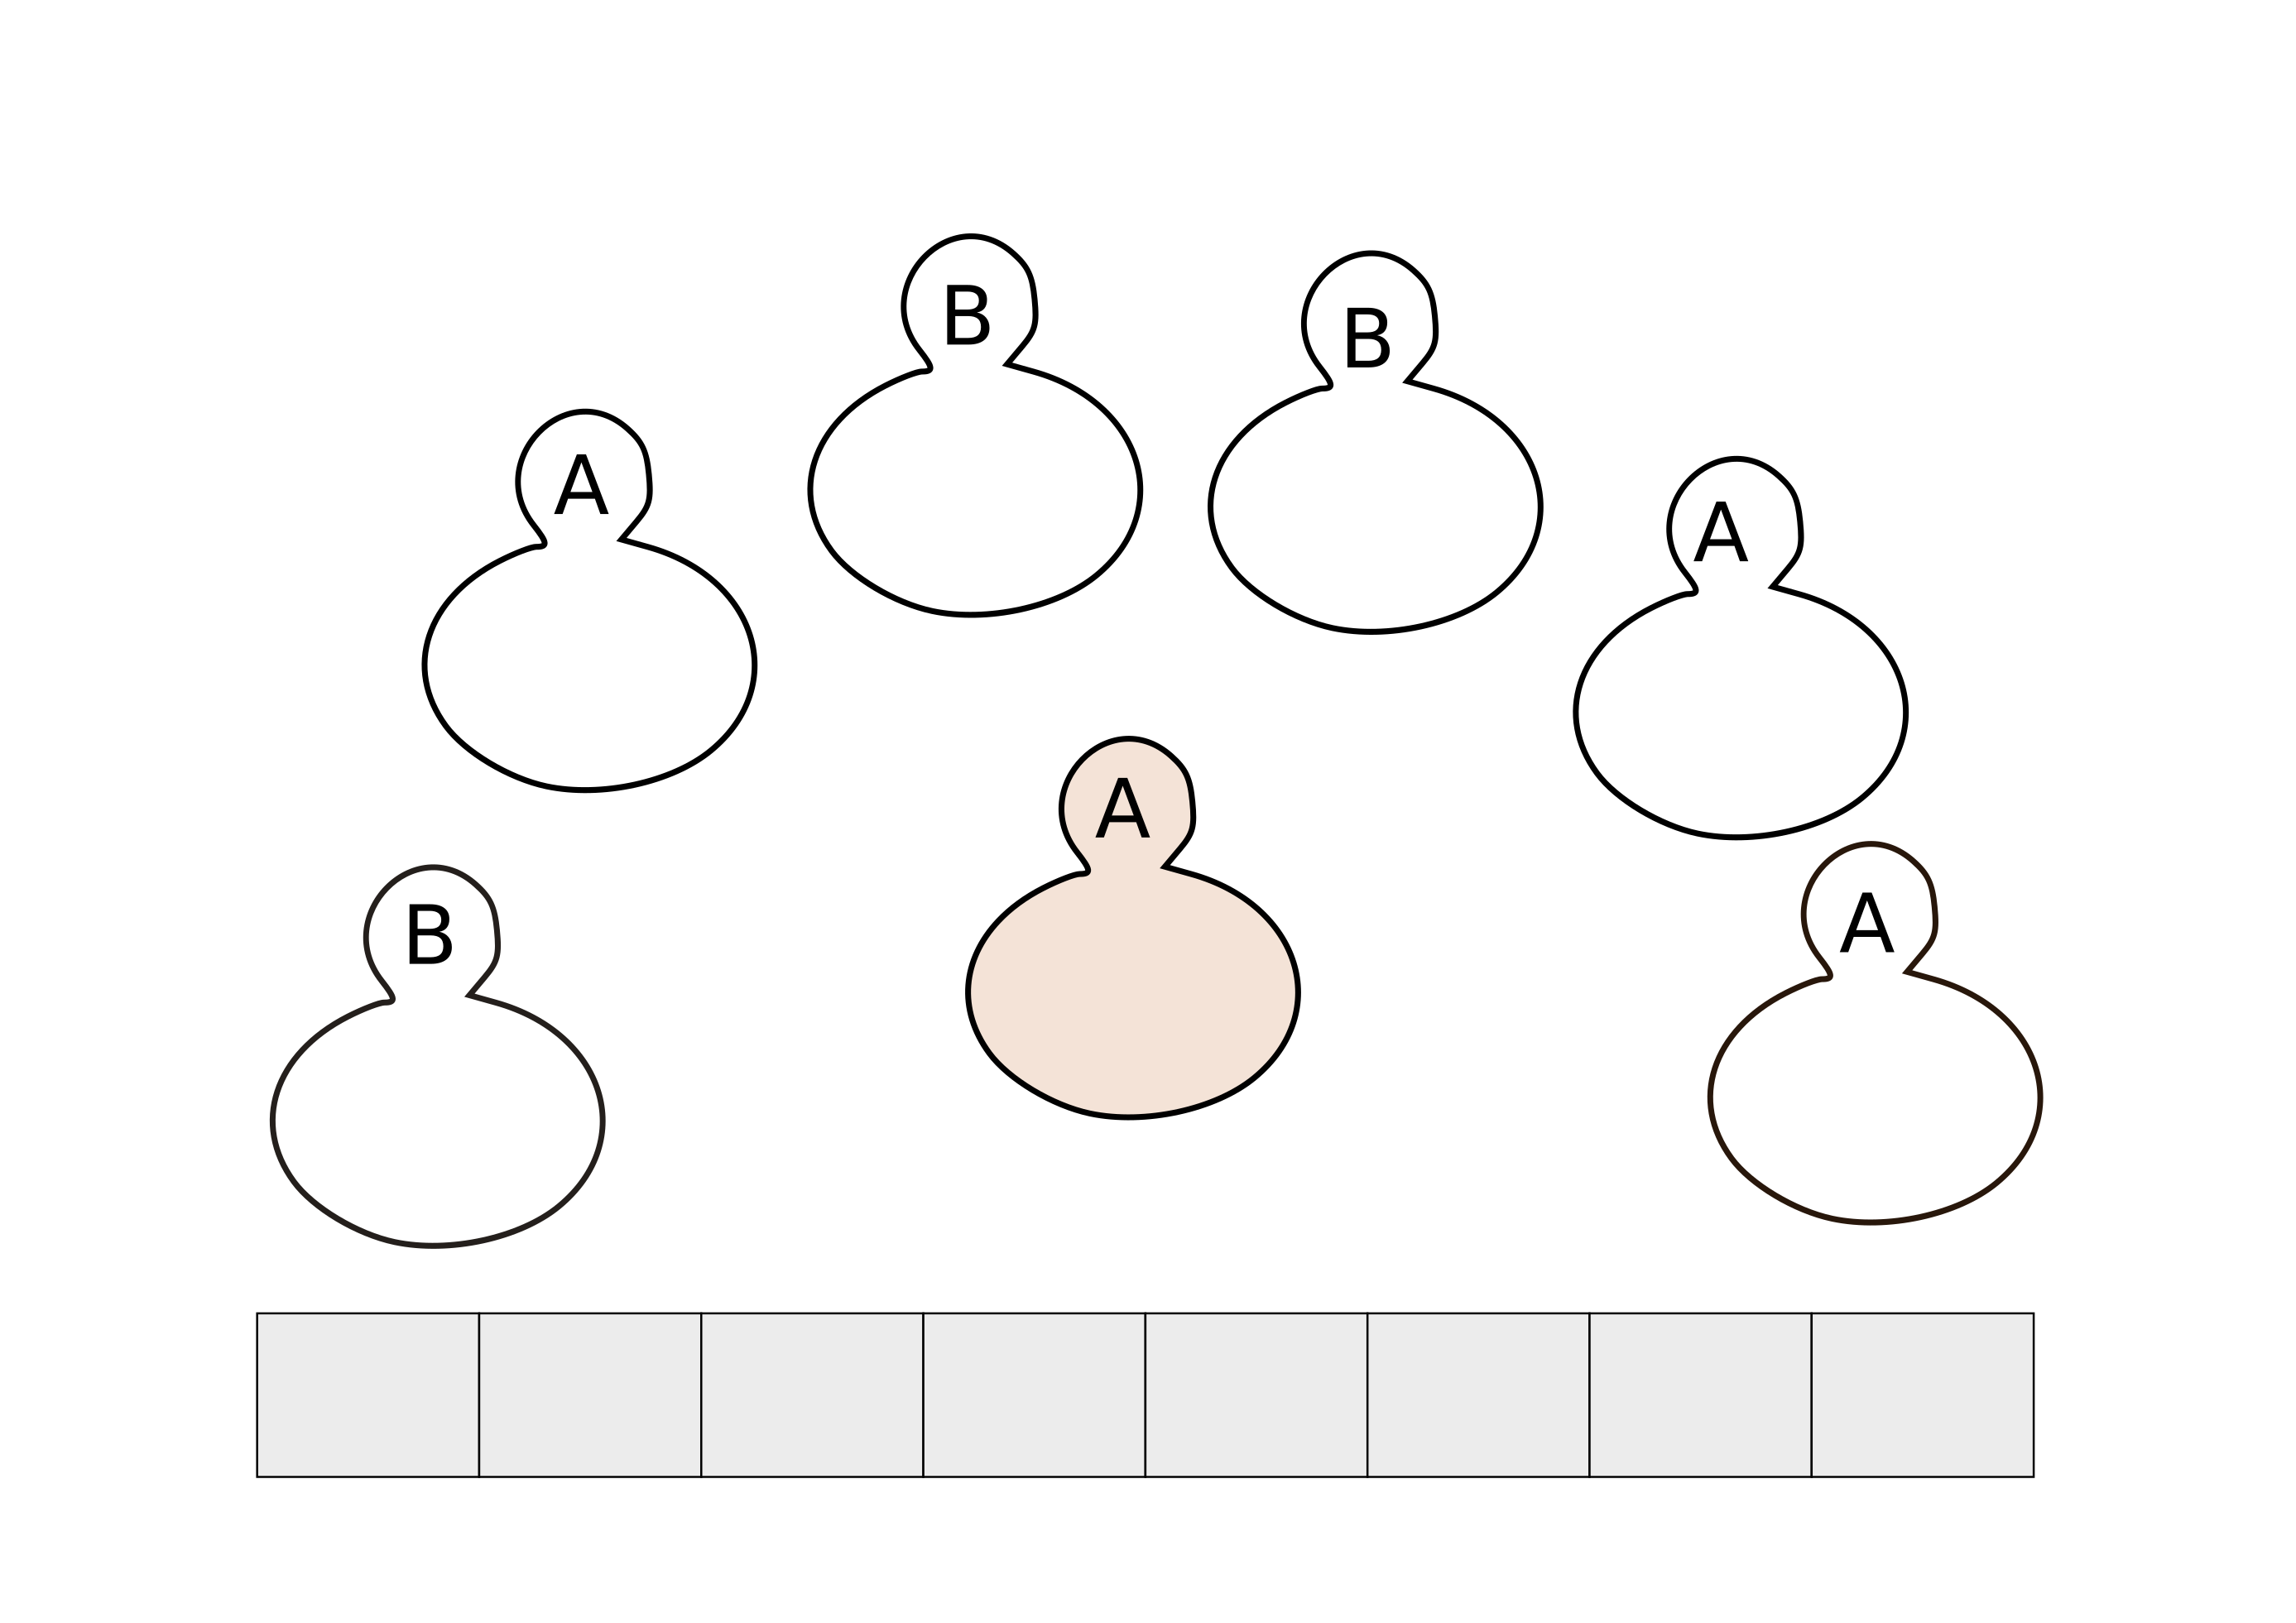
\includegraphics[width=4cm, height=3.5cm]{drawing.png}
  \end{subfigure}
  \begin{subfigure}[b]{0.24\textwidth}
    \caption{}
  	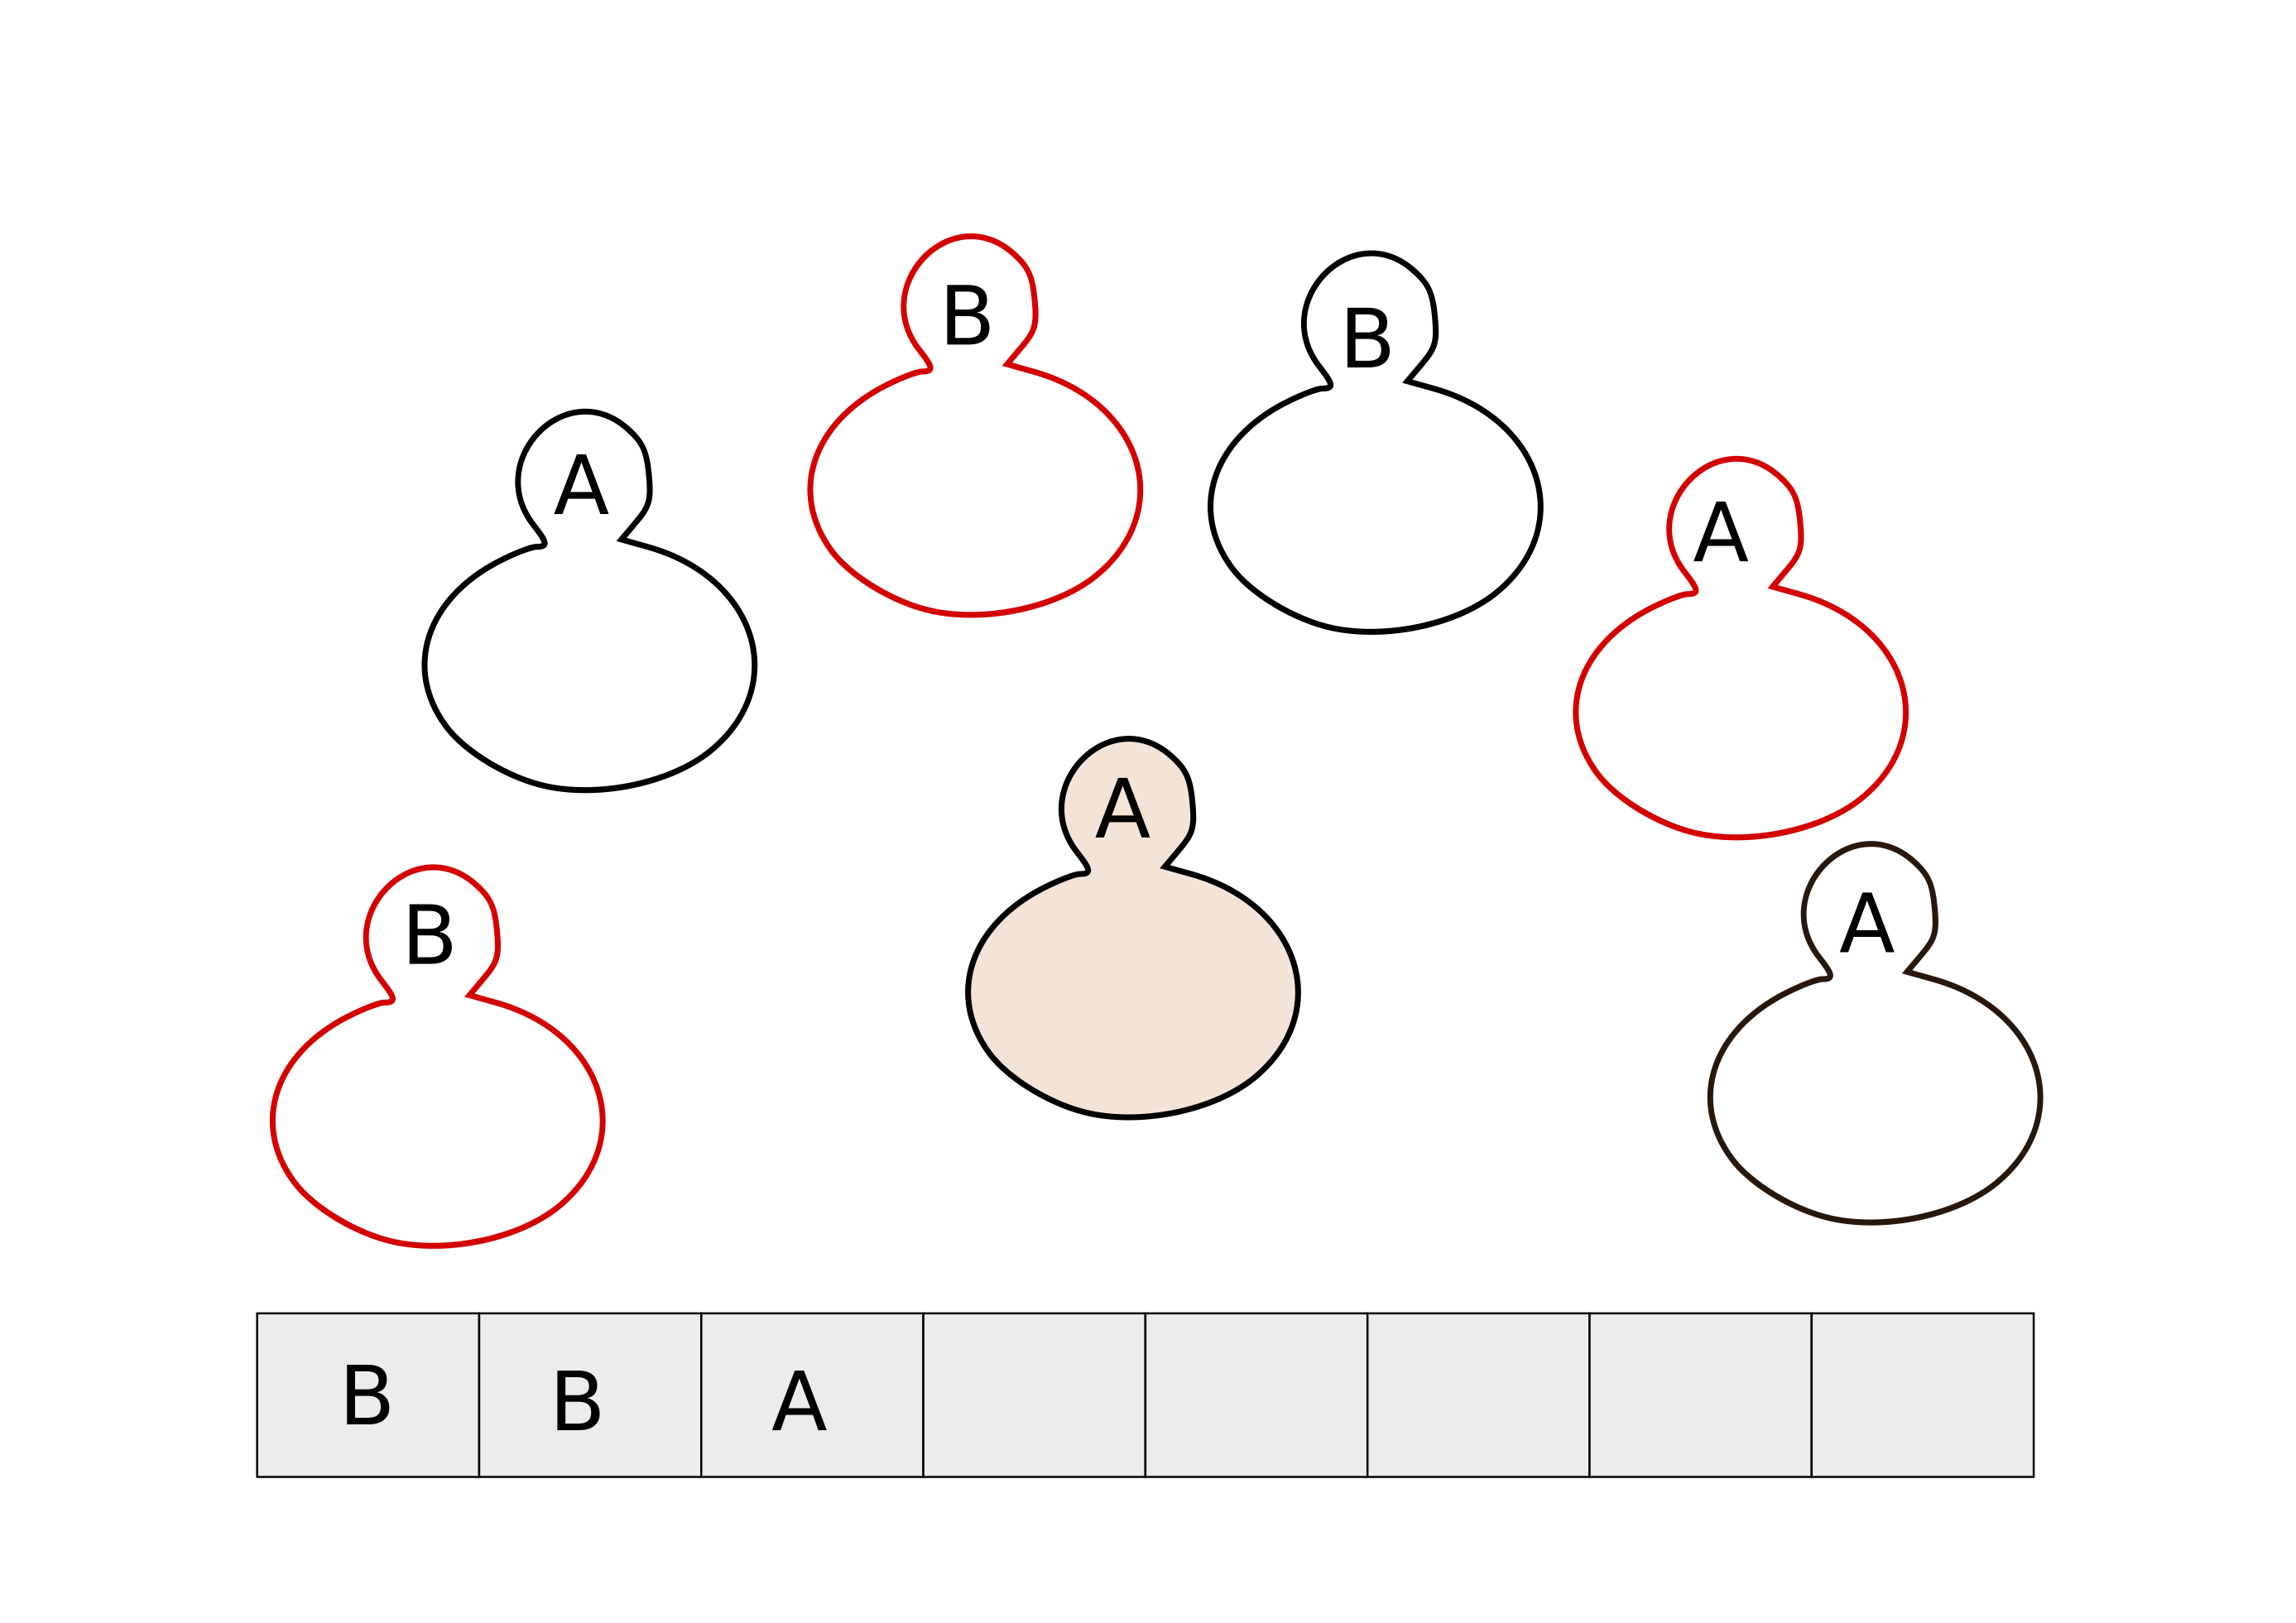
\includegraphics[width=4cm, height=3.5cm]{drawing1.png}
  \end{subfigure}
  \begin{subfigure}[b]{0.24\textwidth}
    \caption{}
  	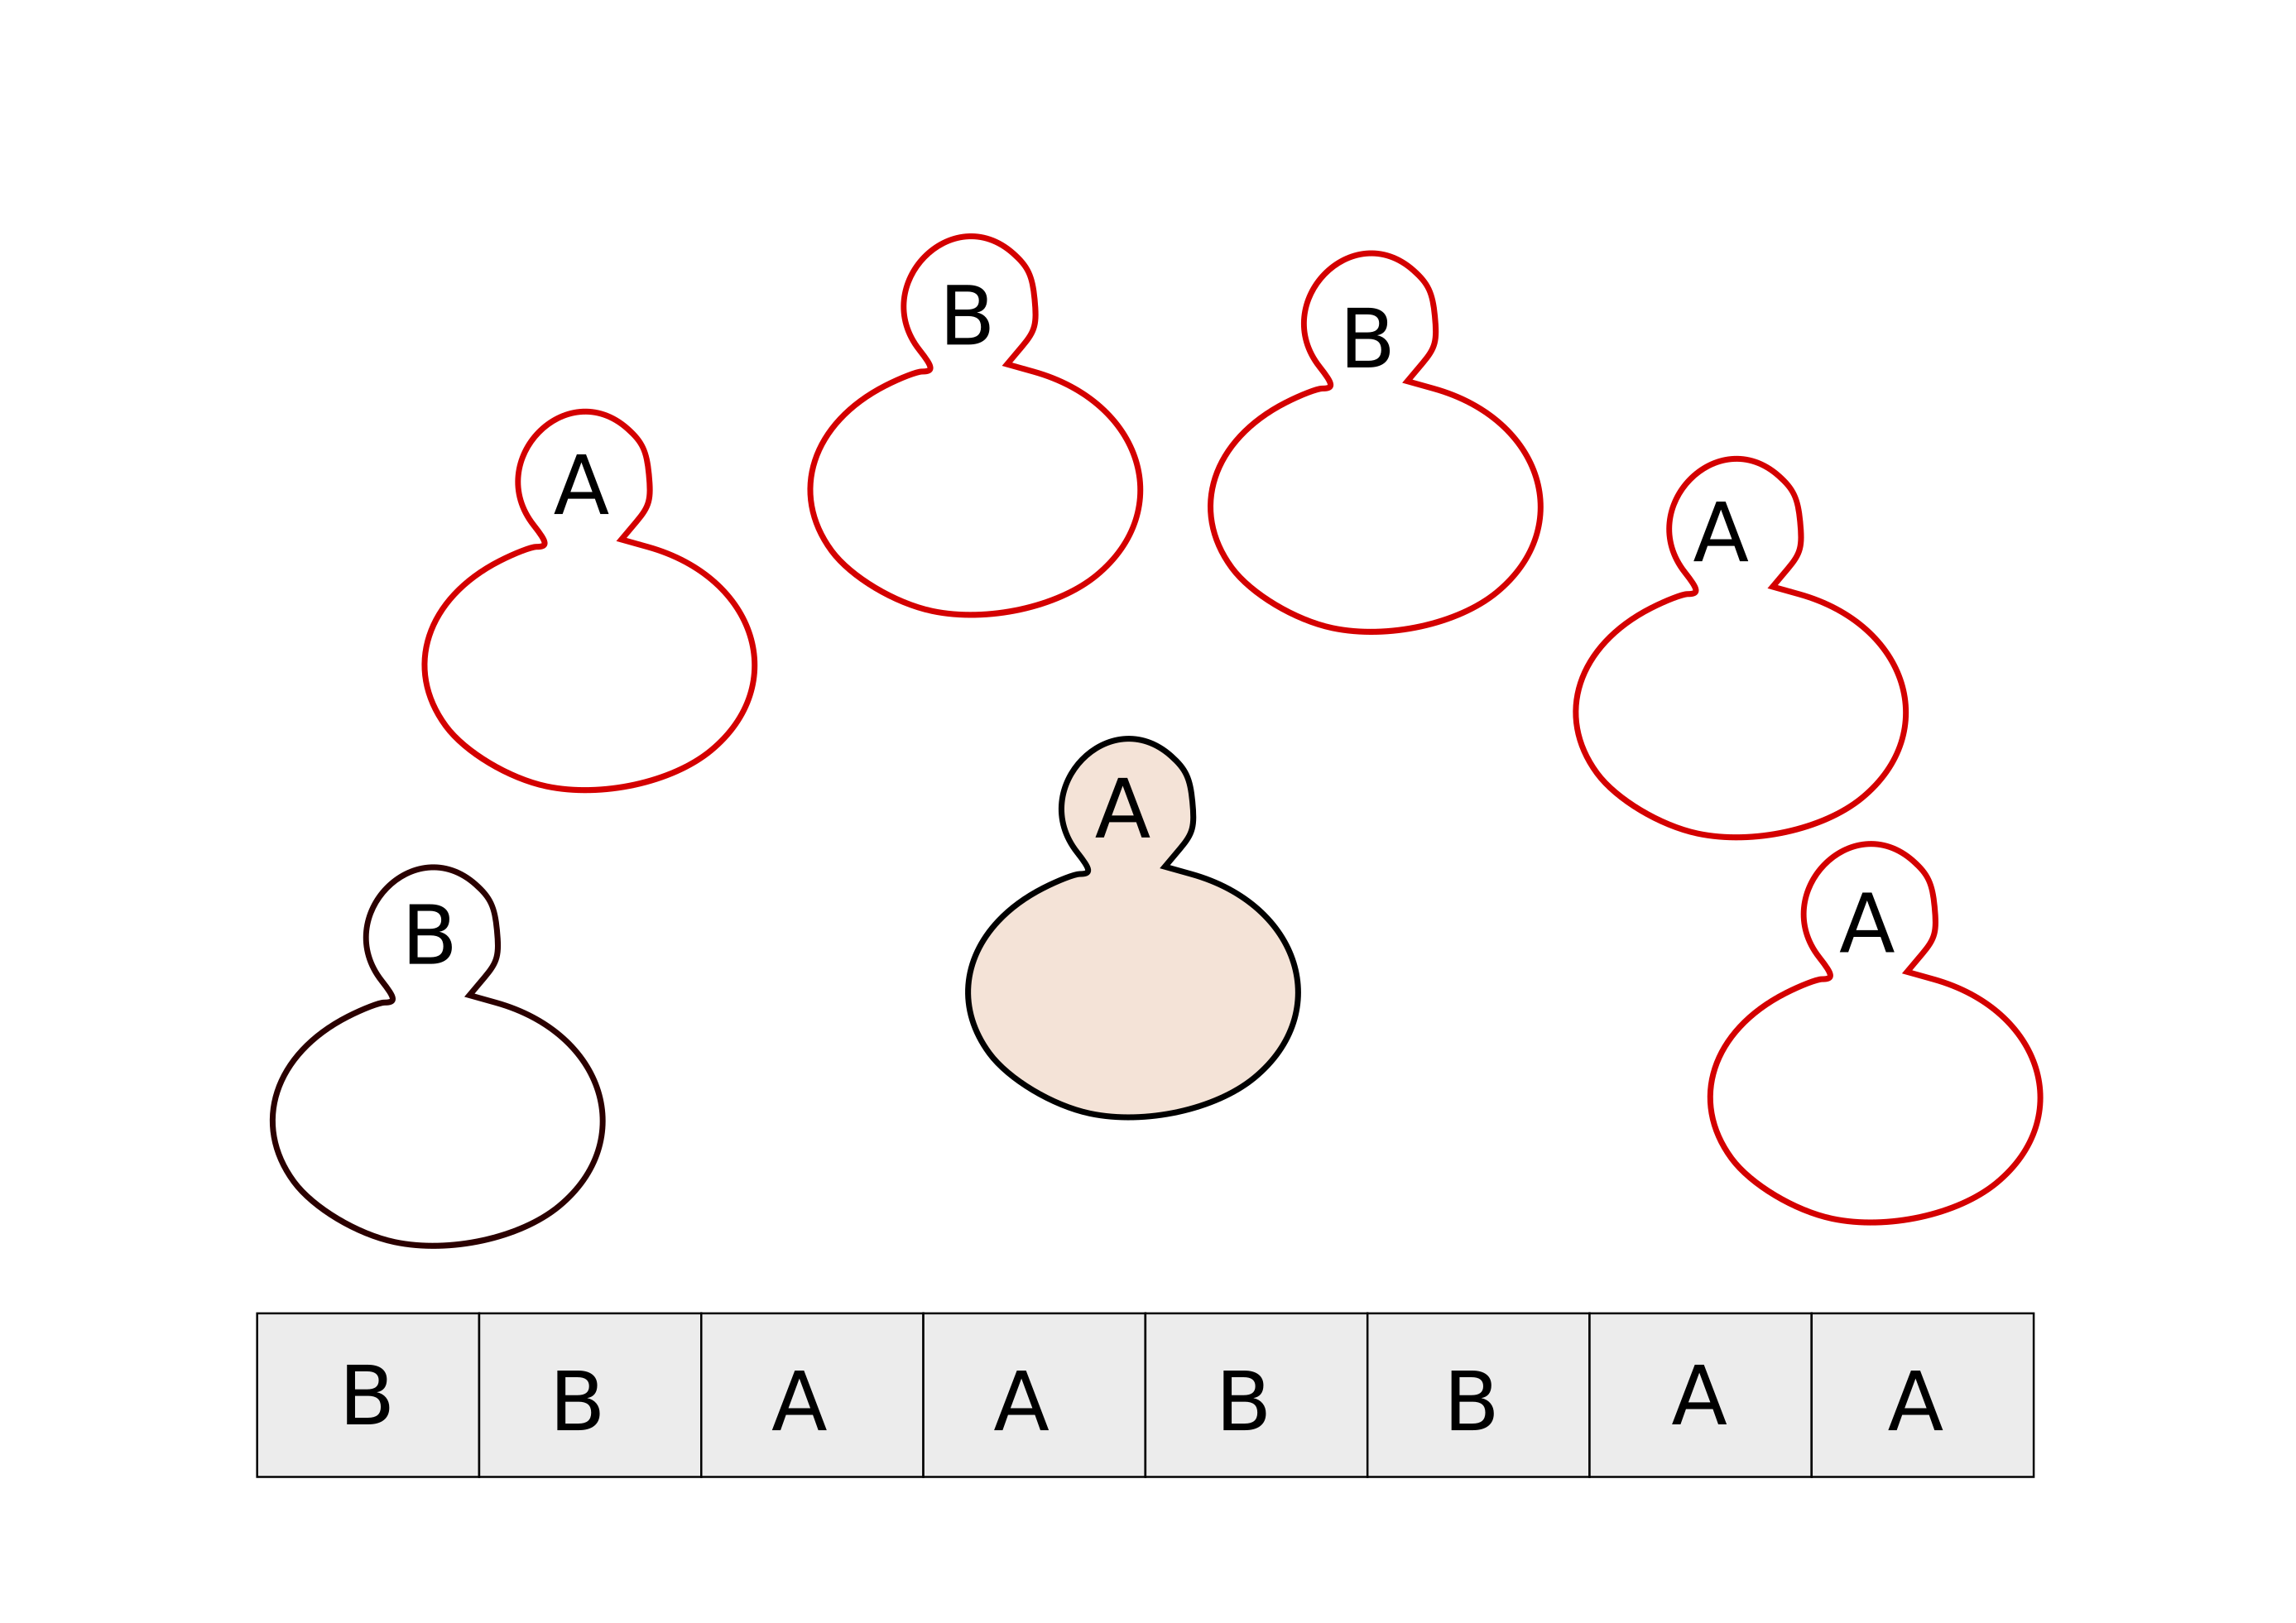
\includegraphics[width=4cm, height=3.5cm]{drawing2.png}
  \end{subfigure}
  \begin{subfigure}[b]{0.24\textwidth}
    \caption{}
  	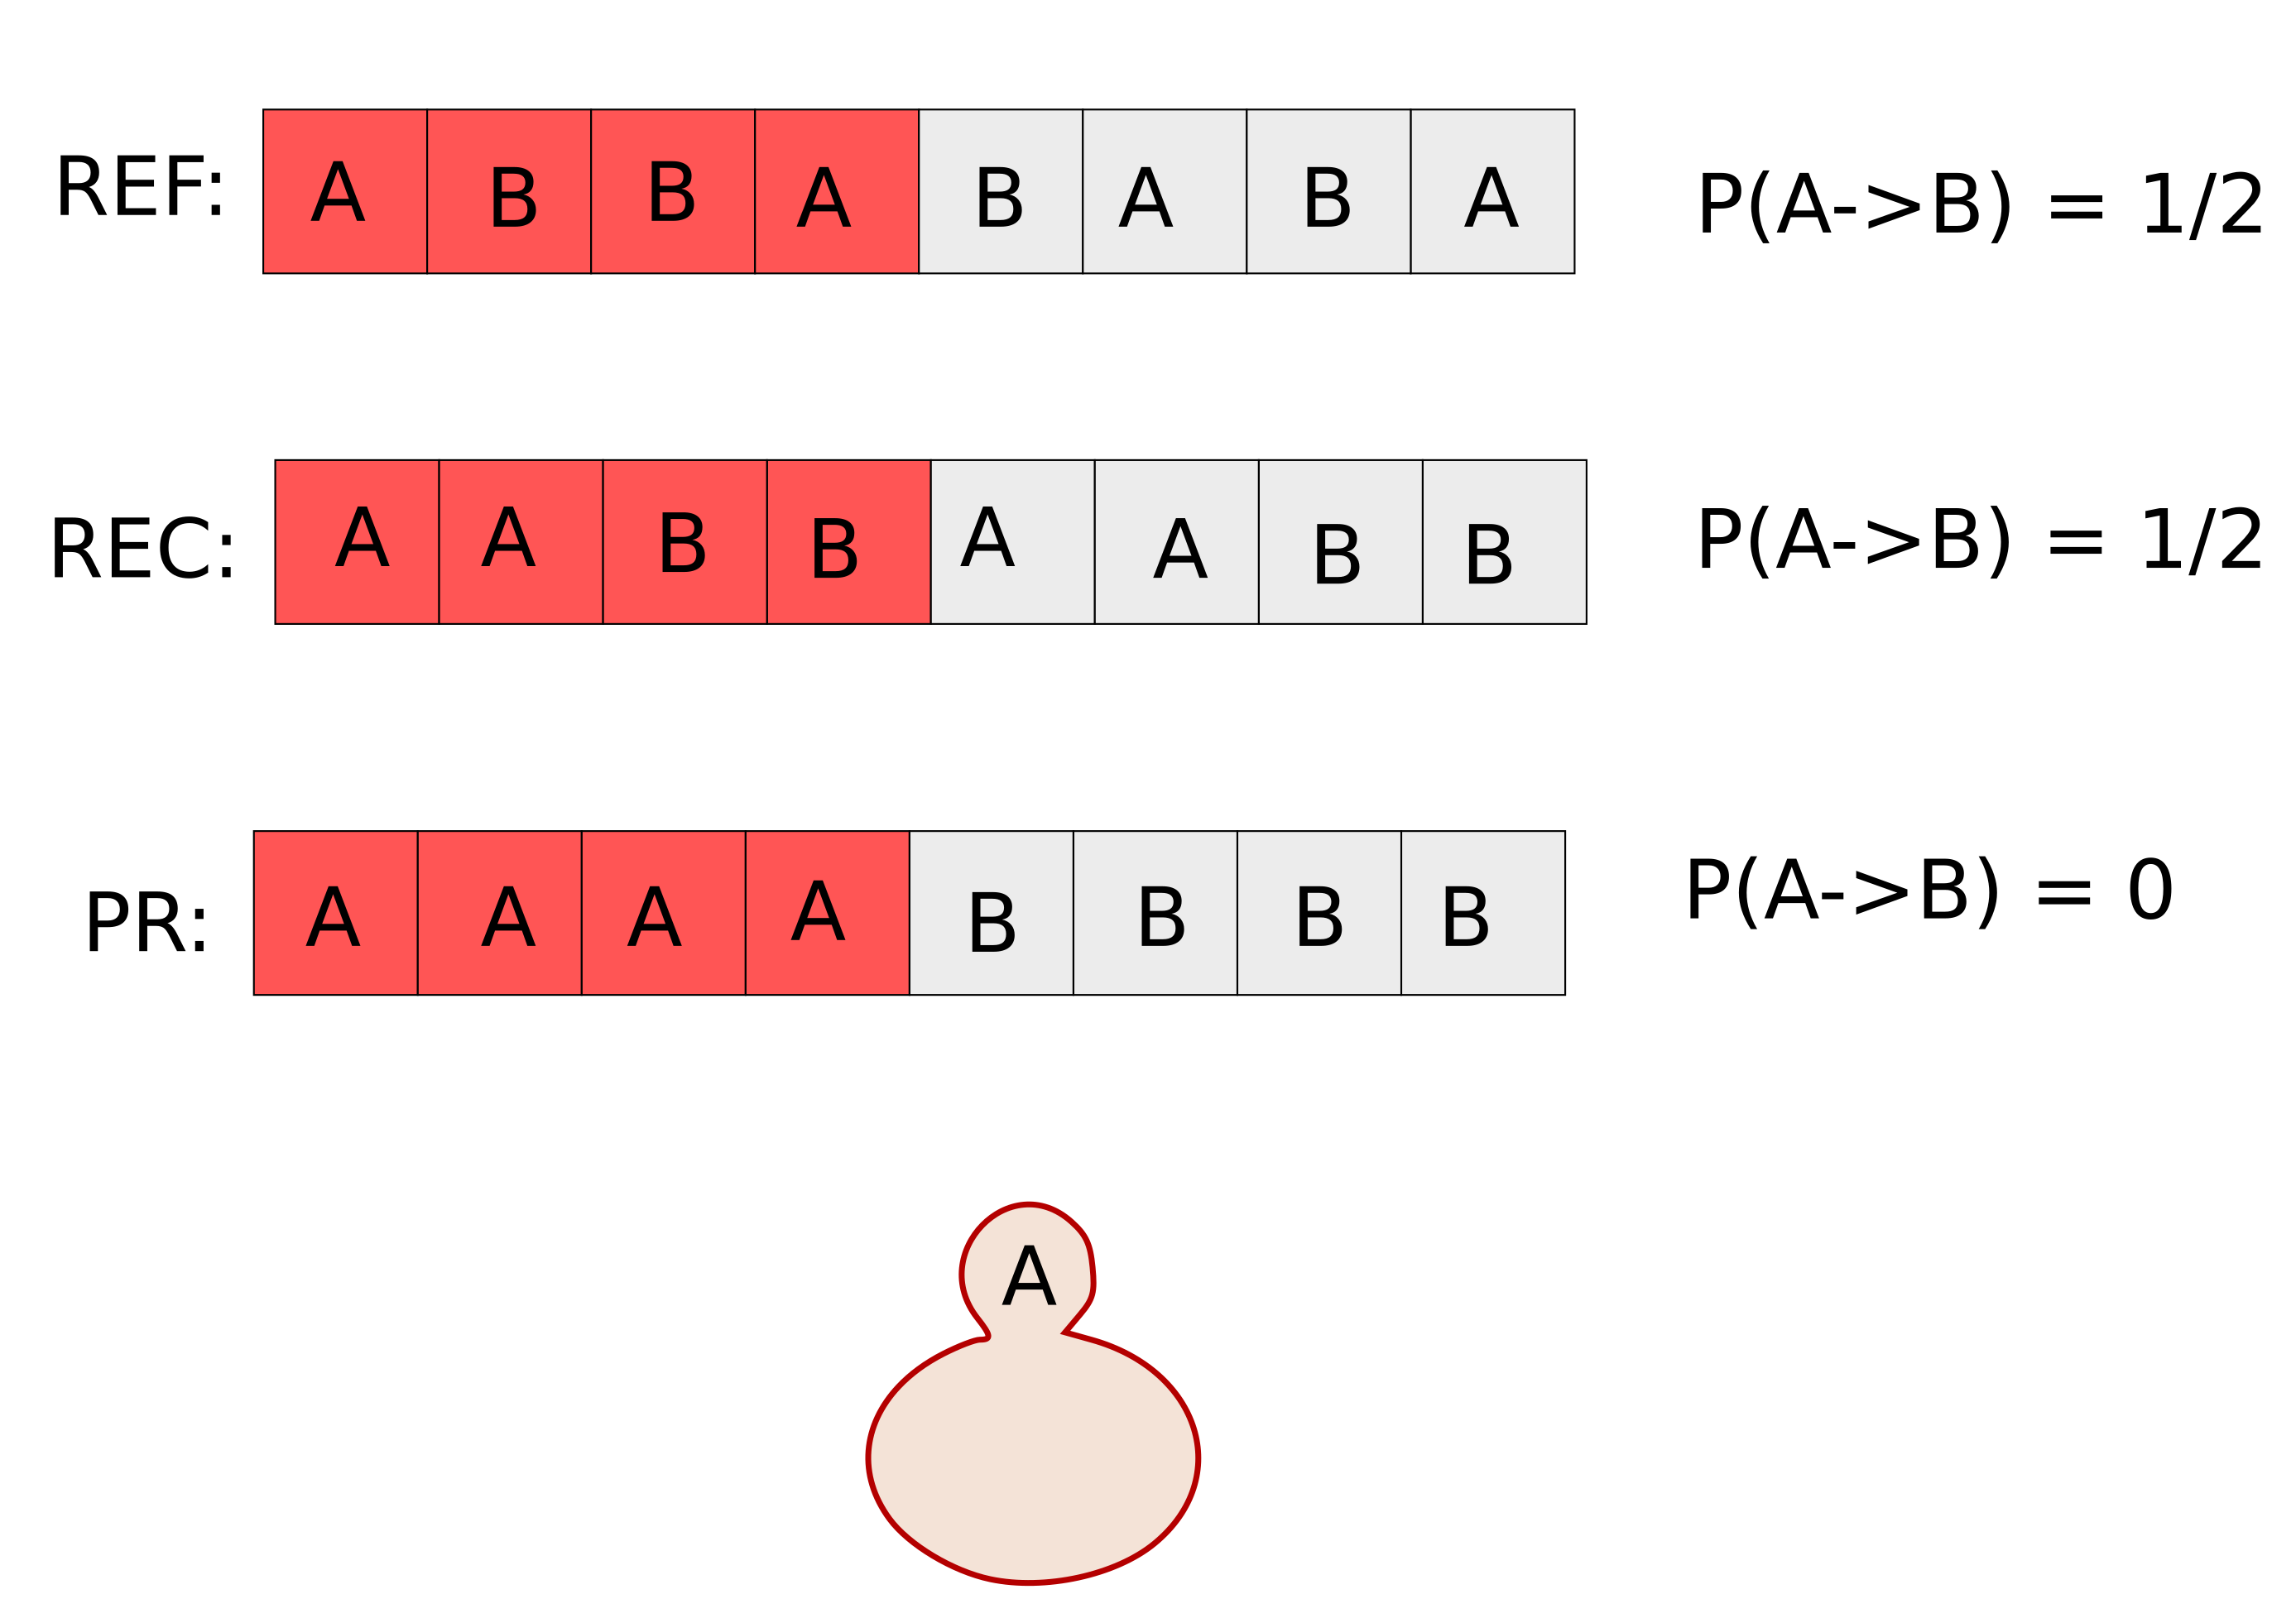
\includegraphics[width=4cm, height=3.5cm]{drawing3.png}
  \end{subfigure}
  \captionsetup{format=plain}
  \caption[Schematic representation of the opinion dynamics model.]{Schematic representation of the opinion dynamics model. Focus lies on the central, colored actor. The grey bar represents its hidden time-line $L_i(t)$. The central actor is connected to six other actors. We assume that these are only connected to this central actor, so their opinion will not be changed until the central actor becomes active. \textbf{(a)} Initial situation: every actor is randomly assigned an opinion; the hidden time-line of the central actor is empty; \textbf{(b)} and \textbf{(c)} Actors become active (indicated in red) and push their opinion on the hidden time-line of the central actor; \textbf{(d)} The central actor becomes active: $S = 4$ items of its hidden time-line are selected and shown on its actual time-line (indicated in red). (i) REF: the hidden time-line is randomly shuffled; (ii) REC: the hidden time-line is ordered from most recent to oldest; (iii) PR: the hidden time-line is ordered according to the current opinion of the central actor. For each filtering algorithm the probability that the central actor changes its opinion is indicated. Only the first four posts are taken into account, the rest is deleted.}
\label{op_dyn_schem}
\end{figure}

\subsection{Stubbornness}

If we introduce stubbornness in the model we mainly use the resistance parameter, as explained in Section \ref{stubbBin}. Lets summarize this concept of stubbornness. Each actor is given a resistance parameter $r_i$, with $0 \leqslant r_i \leqslant 1$; $r_i = 0$ means not stubborn and $r_i = 1$ means completely stubborn. For all intermediate values of $r_i$, a random number $f$ between zero and one is drawn; if $f > r_i$, the actor updates its opinion, if $f \leqslant r_i$, the actor keeps its opinion. \\
\newline
The pseudo-code for updating the opinions of the active actors in case of using a resistance parameter $r$ at time step $t$ is displayed in Algorithm \ref{alg:update}.

\begin{algorithm}[H]
\caption{Updating the opinions of the active actors at time $t$.}
\label{alg:update}
\begin{algorithmic}[1]
	\State \(L_i \leftarrow \text{hidden time-line}\)
	\State \(R_i \leftarrow \text{actual time-line}\)
	\State \(S \leftarrow 20\) \Comment{Maximum length of time-line $R$}
	\State \(r\) \Comment{Stubbornness parameter of each actor, takes values between $0$ and $1$}
	\ForAll{active actor $i$}
		\State \(\text{op} \leftarrow \text{current opinion}\)
		\ForAll{neighbor $k$} \Comment{Add opinion of active actor $i$ to hidden time-line of each neighbor $k$}
			\State \(L_k.\textsc{add}\text{(op)}\)
		\EndFor
		\State \(f \leftarrow \text{rand(0, 1)}\) \Comment{Draw random number between $0$ and $1$}
		\If{$f > r$}
			\State \(\text{op} \leftarrow \Call{Update opinion}{L_i}\) \Comment{Update opinion of active actor $i$}
		\Else
			\State \(\text{op} \leftarrow \text{current opinion}\) \Comment{Do not update opinion of active actor $i$}
		\EndIf
	\EndFor
	
	\Function{Update opinion}{$L_i$}
		\State \(\textsc{Order}(L_i)\) \Comment{Order hidden time-line according to REF, REC or PR filtering}
		\State \(R_i \leftarrow L_i.\textsc{resize}(S)\) \Comment{Time-line $R_i$ = $S$ first elements of ordered hidden time-line}
		\State \(\text{op} \leftarrow \textsc{probMaj}(R_i)\) \Comment{Update opinion according to probabilistic majority model}
	\State \Return op \Comment{Return updated opinion}
	\EndFunction
\end{algorithmic}
\end{algorithm}

\chapter{Results}

This chapter is subdivided into four main sections. We first discuss the impact of network structure on the evolution of the prevalence of the opinions and the formation of echo chambers. Then, we introduce stubbornness. The impact of how the opinions are initially distributed in a network with community structure (SBM) are discussed afterwards. Finally, we study the opinion dynamics model in real-world networks. We discuss the results and compare them to results from network models with similar average degree, clustering or modularity.\\
\newline
Four different network models are studied: (i) Erd\H{o}s-R\'{e}nyi model (ER); (ii) Watts-Strogatz model (WS); (iii) stochastic block model (SBM) and (iv) stochastic Watts-Strogatz block model (SBM-WS). Each model has $N = 10^3$ nodes and average degree $\left<k\right> \sim 10$. The ER model has an edge probability $p = 0.01$. For the WS model, we use two rewiring probabilities: $\beta = 0.01$ ($\left<cc\right> = 0.648 \pm 0.003$) and $\beta = 0.06$ ($\left<cc\right> = 0.557 \pm 0.007$). The SBM has 10 communities of size 100 nodes each. We study one configuration with high modularity ($Q = 0.908 \pm 0.005$, with an edge probability inside the communities $p_{\text{cl}} = 0.1$ and an edge probability between communities $p_{\text{add}} = 0.001$) and one configuration with low modularity ($Q = 0.220 \pm 0.007$, with $p_{\text{cl}} = 0.03$ and $p_{\text{add}} = 0.008$). The SBM-WS has 10 communities of size 100 nodes each. Each community has WS parameters: mean degree $\left<k\right> =10$ and rewire probability $\beta = 0.01$. Edges are added between communities with a probability $p_{\text{add}} = 0.001$ ($\left<cc\right> = 0.553 \pm 0.004$ and $Q = 0.909 \pm 0.004$).\\
\newline
The opinion dynamics model discussed in Section \ref{modelThesis} is used. We set the activation probability equal to $p_{\text{act}} = 0.1$ and the actual time-line of each actor has a maximum length equal to $S=20$. If another model is used or if parameters (either those of the network models or the opinion dynamics model) are changed, this will be explicitly stated in the relevant sections. Opinions and stubborns (if present) are randomly distributed over the network, unless specified otherwise.

\section{Network structure}\label{netw_struc}

Real-world social networks often have high clustering and modular structure. We want to study the impact of these topologies on the dynamics of opinions. In this section, we will discuss results related to different network topologies with focus on the effect of clustering and community structure. Two different opinion distributions are investigated, balanced and unbalanced starting conditions. For both starting conditions we investigate the evolution of the prevalence of the opinions and the formation of echo chambers. Two filtering algorithms will be compared, the REC and the PR filtering algorithms, to investigate the interplay between filtering algorithms and network structure.

\subsection{Balanced starting conditions}
\label{50-50}

In this configuration $50 \%$ of the actors start with opinion A ($P_{\text{A}}(0) = 0.5$) and $50 \%$ of the actors start with opinion B ($P_{\text{B}}(0) = 0.5$).\\
\newline
\textbf{Evolution of the prevalence of the opinions}\\
\newline
We start with the results for the evolution of the prevalence of the opinions. For both the REC and the PR filtering algorithms, the community structure is not able to break the status quo. The initial prevalence of the opinions is maintained over time (Fig. \ref{ev_op_50_50}). This is also the case for networks with high clustering \cite{Perra2019}. 

\begin{figure}[H]
  \begin{subfigure}[b]{0.49\textwidth}
    \caption{}
    \includegraphics[width=8cm, height=7cm]{fraction_of_opinions_SBM_10x100_01-0001_003-0008_50-50_PR_REC_8x7.png}
    \label{sbm_50-50}
  \end{subfigure}
  \begin{subfigure}[b]{0.49\textwidth}
    \caption{}
    \includegraphics[width=8cm, height=7cm]{fraction_of_opinions_SBM-WS_10x100_10-001-0001_50-50_PR_REC.png}
    \label{sbm-ws_50-50}
  \end{subfigure}
  \captionsetup{format=plain}
  \caption[Evolution of the prevalence of opinion A ($P_{\text{A}}(t)$) for balanced starting conditions.]{Evolution of the prevalence of opinion A ($P_{\text{A}}(t)$) for balanced starting conditions. \textbf{(a)} SBM; \textbf{(b)} SBM-WS. Two configurations are implemented for the SBM: a high modularity ($Q = 0.908 \pm 0.005$)) and a low modularity ($Q = 0.220 \pm 0.007$) configuration. For each model the REC and the PR filtering algorithms are compared. The dotted black line represents the initial prevalence of opinion A. Each curve is the average of $10^2$ independent simulations and data points are shown for every 50 time steps to improve visualization. Bars represent the standard deviation $\sigma$.}
\label{ev_op_50_50}
\end{figure}
\noindent
\textbf{Echo chambers}\\
\newline
Fig. \ref{echo_50_50} shows the distribution of the fraction of friends (nearest neighbors, nn) of actor $i$ with the same opinion B at $t=500$, $\left<P_{\text{B}}^{\text{nn}}\right>$. The region on the $x$-axis close to zero describes neighborhoods in which none, or few actors, adopt opinion B (these are thus neighborhoods in which most actors adopt opinion A). Conversely, the region on the $x$-axis close to one describes neighborhoods in which a majority of the actors adopt opinion B. The distribution is obtained by imposing ten equispaced bins, $\Delta x = 0.1$ \cite{Perra2019}. 

\begin{figure}[H]
  \begin{subfigure}[b]{0.49\textwidth}
    \caption{}
  	\includegraphics[width=8cm, height=7cm]{echo_chambers_no_stubb_50-50_REC_8x7.png}
      \end{subfigure}
  \begin{subfigure}[b]{0.49\textwidth}
    \caption{}
  	\includegraphics[width=8cm, height=7cm]{echo_chambers_no_stubb_50-50_PR_8x7.png}
  \end{subfigure}
  \captionsetup{format=plain}
  \caption[Distribution of the fraction of friends (nearest neighbors, nn) of actor $i$ with the same opinion B at $t=500$, $\left<P_{\text{B}}^{\text{nn}}\right>$, for balanced starting conditions.]{Distribution of the fraction of friends (nearest neighbors, nn) of actor $i$ with the same opinion B at $t = 500$, for balanced starting conditions. \textbf{(a)} REC filtering algorithm; \textbf{(b)} PR filtering algorithm. Four network models are used: (i) ER; (ii) SBM; (iii) SBM-WS and (iv) WS. Two configurations are implemented for the SBM: a high modularity ($Q = 0.908 \pm 0.005$)) and a low modularity ($Q = 0.220 \pm 0.007$) configuration. For the WS model, we use two different values for the rewire probability: $\beta = 0.01$ ($\left<cc\right> = 0.648 \pm 0.003$; WS2) and $\beta = 0.06$ ($\left<cc\right> = 0.557 \pm 0.007$; WS1). The distribution is normalized by dividing for the same quantity computed at $t=0$. The dotted black line ($y=1$) represents a constant amount of echo chambers over time. Each curve is the average of $10^2$ independent simulations. Error bars are omitted for improved visualization.}
\label{echo_50_50}
\end{figure}
\noindent
Two filtering algorithms are compared, the REC and the PR filtering algorithms. The results for both filtering algorithms are qualitatively the same. The difference is that the formation of echo chambers, using the PR filtering algorithm, is about ten times as large compared to the formation of echo chambers using the REC filtering algorithm. \\
\newline
The ER model shows no, or a limited, sign of the formation of echo chambers, for both the REC and PR filtering algorithms. Networks with high clustering (WS and SBM-WS), on the other hand, show a sign of polarization and formation of echo chambers (visible in the two spikes, one around zero and another around one). Going to higher values of the clustering coefficient ($\left<cc\right> = 0.557 \pm 0.007$ to $\left<cc\right> = 0.648 \pm 0.003$) in the WS model results in significantly larger echo chambers. This suggests that the formation of echo chambers is sensitive to changes in the clustering coefficient. The SBM with high modularity, community structure, shows an appearance of polarization (mainly when using the PR filtering algorithm), however, the formation of echo chambers is significantly smaller compared to networks with high clustering. The stochastic block model with low modularity has no, or limited, formation of echo chambers, similar as for the ER model. This is expected, since a SBM with low modularity, and hence, almost non-existing community structure, resembles an ER network. The SBM-WS has both community structure and high average clustering. The formation of echo chambers when using this model is approximately of the same size as the formation of echo chambers in a WS model with similar average clustering. This suggests that it is the high clustering that drives the dynamics to form echo chambers, while the community structure plays a less important role. \\
\newline
For balanced starting conditions, none of the network models, nor the filtering algorithms could break the status quo (Fig. \ref{ev_op_50_50} and related results in \cite{Perra2019}). Despite this preserving of the balanced opinion distribution, the interplay of filtering algorithms and network structure can shift the initial randomly distributed opinions to a clustered opinion distribution and thus lead to polarization and formation of echo chambers.

\subsection{Unbalanced starting conditions}\label{20-80}

We will now investigate the effect of unbalanced starting conditions, that is one opinion is initially more prevalent than the other. The initial prevalence of opinion A is $P_\text{A}(0) = 0.2$, the minority opinion, and of opinion B is $P_\text{B}(0) = 0.8$, the majority opinion.\\ 
\newline
\textbf{Evolution of the prevalence of the opinions}\\
\newline
Fig. \ref{ev_op_20_80} shows the results for the evolution of the prevalence of opinion A, which is the minority opinion. For each network model the REC and PR filtering algorithms are compared. \\
\newline
The REC filtering algorithm maintains the status quo; the prevalence of opinion A remains stable over time for the four network models. When using the PR filtering algorithm, results are different. The prevalence of the minority opinion, $P_\text{A}(t)$, decreases over time. This decrease is a consequence of the PR filtering algorithm. Since the PR filtering algorithm orders the posts according to the actors' preferences, actors with the majority opinion B will mainly see posts with the same opinion B on their time-line. This limits the chance of changing their opinion to the minority opinion. Actors with the minority opinion A will see posts with opinion A on their time-line when using the PR filtering algorithm. However, because there are more actors with opinion B than actors with opinion A, the actors with the minority opinion A will also see a number of posts with the majority opinion B on their time-line. When using the PR filtering algorithm, there is an imbalance in the sense that actors with the minority opinion A have a chance of switching to the majority opinion B, whereas actors with the majority opinion B have (almost) no chance of switching to the minority opinion A. This imbalance leads to the decrease of the minority opinion A.\\
\newline
Fig. \ref{ev_op_20_80} shows that the minority opinion A eventually vanishes. This is the case for the low clustering networks, with $P_\text{A}(500) = 0.001 \pm 0.003$ for the ER network, $P_\text{A}(500) = 0.002 \pm 0.003$ for the SBM with low modularity and $P_\text{A}(500) = 0.003 \pm 0.006$ for the SBM with high modularity. The high clustering in the WS and SBM-WS networks seems to slightly hamper this vanishing of the minority opinion with an average value of $P_\text{A}(500) = 0.007 \pm 0.014$ for the SBM-WS network (Fig. \ref{sbm-ws_20-80_op}) and an average value of $P_\text{A}(500) = 0.009 \pm 0.015$ for the WS network (Fig. \ref{ws_20-80_op}).

\begin{figure}[H]
  \begin{subfigure}[t]{0.49\textwidth}
    \subcaption{}
  	\includegraphics[width=8cm, height=7cm]{fraction_of_opinions_ER_001_50-50_PR_REC_20-80_8x7.png}
      \end{subfigure}
  \begin{subfigure}[t]{0.49\textwidth}
    \subcaption{}
  	\includegraphics[width=8cm, height=7cm]{fraction_of_opinions_WS_10-006_PR_REC_20-80_8x7.png}
    \label{ws_20-80_op}
  \end{subfigure}
  \begin{subfigure}[t]{0.49\textwidth}    
    \subcaption{}
    \includegraphics[width=8cm, height=7cm]{fraction_of_opinions_SBM_01-0001_003-0008_PR_REC_20-80_8x7.png}
  \end{subfigure}
  \begin{subfigure}[t]{0.49\textwidth}
    \subcaption{}
    \includegraphics[width=8cm, height=7cm]{fraction_of_opinions_SBM-WS_10-001-0001_PR_REC_20-80_8x7.png}
    \label{sbm-ws_20-80_op}
  \end{subfigure}
  \captionsetup{format=plain}
  \caption[Evolution of the prevalence of opinion A ($P_\text{A}(t)$) for unbalanced starting conditions.]{Evolution of the prevalence of opinion A ($P_\text{A}(t)$) for unbalanced starting conditions. \textbf{(a)} ER; \textbf{(b)} WS; \textbf{(c)} SBM; \textbf{(d)} SBM-WS. The WS model has $\beta = 0.06$ ($\left<cc\right> = 0.557 \pm 0.007$). Two configurations are implemented for the SBM: a high modularity ($Q = 0.908 \pm 0.005$) and a low modularity ($Q = 0.220 \pm 0.007$) configuration. For each model the REC and the PR filtering algorithms are compared. The dotted black line represents the initial prevalence of opinion A. Each curve is the average of $10^2$ independent simulations and data points are shown for every 50 time steps to improve visualization. Bars represent the standard deviation $\sigma$.}
\label{ev_op_20_80}
\end{figure}
\noindent
This result differs from results in \cite{Perra2019}, where the minority opinion was able to survive over time for all the network models, even for the PR filtering algorithm, and where a minority opinion prevalence at $t=500$ between $P_\text{A}(500) = 0.06$ and $P_\text{A}(500) = 0.09$ was reported \cite{Perra2019}. The difference in the results is most likely due to an interplay between the network size $N$, the average degree $\left<k\right>$ and the maximum length of the actual time-line $S$. The results that where obtained in \cite{Perra2019} are for networks with size $N = 10^5$ nodes and average degree $\left<k\right> \sim 6$. In this thesis results are obtained for $N=10^3$ and average degree $\left<k\right> \sim 10$. In both cases the maximum length of the actual time-line is $S=20$. Fig. \ref{ev_op_WS_k=6} shows the results for the evolution of the prevalence of opinion A for an initial $20/80$ opinion distribution and using the PR filtering algorithm; Fig. \ref{ws1000} displays results for a WS model with $N=10^3$ and $\left<k\right> = 6$; Fig. \ref{ws10000} shows results for a WS model with $N=10^4$ and $\left<k\right> = 6$. We see that the minority opinion A reaches higher final values of $P_0(500)$ compared to the case depicted in Fig. \ref{ws_20-80_op}, with a value of $P_\text{A}(500) = 0.027 \pm 0.023$ in Fig. \ref{ws1000} and a value of $P_\text{A}(500) = 0.030 \pm 0.018$ in Fig. \ref{ws10000}.

\begin{figure}[H]
  \begin{subfigure}[b]{0.49\textwidth}
    \caption{}
  	\includegraphics[width=8cm, height=7cm]{fraction_of_opinions_WS_1000-6_PR_20-80_8x7.png}
    \label{ws1000}
  \end{subfigure}
  \begin{subfigure}[b]{0.49\textwidth}
    \caption{}
  	\includegraphics[width=8cm, height=7cm]{fraction_of_opinions_WS_10000-6_PR_20-80_8x7.png}
    \label{ws10000}
  \end{subfigure}
  \captionsetup{format=plain}
  \caption[Evolution of the prevalence of opinion A ($P_\text{A}(t)$) for unbalanced starting conditions. A WS model with $N=10^3$ or $N=10^4$, $\left<k\right>=6$ and $\beta = 0.01$ is implemented. The PR filtering algorithm is used.]{Evolution of the prevalence of opinion A ($P_\text{A}(t)$) for unbalanced starting conditions. Results for WS with $\left<k\right> = 6$ and $\beta = 0.01$ are depicted with \textbf{(a)} $N=10^3$; \textbf{(b)} $N=10^4$. In both networks the average clustering coefficient is $\left<cc\right> = 0.584 \pm 0.003$. The PR filtering filtering algorithm is used. The dotted black represents the initial prevalence of opinion A. The dotted grey line represents a vanished prevalence of opinion A. Each curve is the average of $10^2$ independent simulations and data points are shown for every 50 time steps to improve visualization. Bars represent the standard deviation $\sigma$.}
\label{ev_op_WS_k=6}
\end{figure}
\noindent
\textbf{Echo chambers}\\
\newline
Fig. \ref{echo_20_80} shows the distribution of the fraction of friends of actor $i$ with the same opinion B at $t=500$.  The REC and PR filtering algorithms are compared for the ER, WS, SBM and SBM-WS.\\
\newline
The results for the ER model and the SBM (both the high and low modularity configuration) look qualitatively the same. Similarly, the results for the WS model and the SBM-WS agree with each other as well. This difference in results between ER/SBM (negligible clustering) and WS/SBM-WS (high clustering) suggests that it is the clustering that drives these differences.\\
\newline
There are no visible effects of having community structure. Fig. \ref{sbm} shows the results for a SBM with high modularity (community structure) and low modularity (negligible community structure). There is (almost) no difference in the results for high and low modularity.

\begin{figure}[H]
  \begin{subfigure}[b]{0.49\textwidth}
    \caption{}
  	\includegraphics[width=8cm, height=7cm]{echo_chambers_no_stubb_ER_001_20-80_PR_REC.png}
    \label{er_echo_20-80}
  \end{subfigure}
  \begin{subfigure}[b]{0.49\textwidth}
    \caption{}
  	\includegraphics[width=8cm, height=7cm]{echo_chambers_no_stubb_WS_10_006_20-80_PR_REC_8x7.png}
    \label{ws}
  \end{subfigure}
  \begin{subfigure}[b]{0.49\textwidth}
    \caption{}
    \includegraphics[width=8cm, height=7cm]{echo_chambers_no_stubb_SBM_01-0001_003-0008_10x100_20-80_PR_REC_8x7.png}
  	\label{sbm}    
  \end{subfigure}
  \begin{subfigure}[b]{0.49\textwidth}
    \caption{}
    \includegraphics[width=8cm, height=7cm]{echo_chambers_no_stubb_SBM-WS_10_001_0001_10x100_20-80_PR_REC_8x7.png}
    \label{sbm-ws}
  \end{subfigure}
  \captionsetup{format=plain}
  \caption[Distribution of the fraction of friends (nearest neighbors, nn) of actor $i$ with the same opinion B at $t=500$, $\left<P_\text{B}^{\text{nn}}\right>$, for unbalanced starting conditions.]{Distribution of the fraction of friends (nearest neighbors, nn) of actor $i$ with the same opinion B at $t = 500$ for unbalanced starting conditions. \textbf{(a)} ER; \textbf{(b)} WS; \textbf{(c)} SBM; \textbf{(d)} SBM-WS. The WS model has $\beta = 0.06$ ($\left<cc\right> = 0.557 \pm 0.007$). Two configurations are implemented for the SBM: a high modularity ($Q = 0.908 \pm 0.005$) and a low modularity ($Q = 0.220 \pm 0.007$) configuration. For each model the REC and the PR filtering algorithms are compared. The distribution is normalized by dividing for the same quantity computed at $t=0$. The dotted black line ($y=1$) represents a constant amount of echo chambers over time. Each curve is the average of $10^2$ independent simulations. Error bars are omitted for improved visualization.}
\label{echo_20_80}
\end{figure}
\noindent
Lets first discuss results for the ER model and the SBM (Fig. \ref{er_echo_20-80} and Fig. \ref{sbm}). When using the REC filtering algorithm, the formation of echo chambers around the majority opinion B is hampered. This is probably a consequence of the absence of clustering and the presence of short average path lengths in these models. There is even a little spike around $\left<P_\text{B}^{\text{nn}}\right> = 0.1$, which indicates a small increase in the fraction of actors with the majority of their neighbors carrying the minority opinion A. From Fig. \ref{ev_op_20_80} it was concluded that the REC filtering algorithm does not break the initial prevalence of the opinions. The opinion distribution is however slightly shifted from the case where the minority opinion A is randomly distributed over the network to the case where the minority opinion A starts to group together in opinion clusters. \\
\newline
The PR filtering algorithm shows a different tendency. There is an increase in the fraction of actors with all their neighbors carrying the majority opinion B. This is a consequence from the fact that the PR filtering algorithm reduces the visibility of the minority opinion A in the neighborhood of actors with the majority opinion B. This reduced visibility of the minority opinion A in these neighborhoods drives them eventually to adopt opinion B, with an increase in the number of echo chambers around the majority opinion B as a consequence. Remember from Fig. \ref{ev_op_20_80}, that the PR filtering algorithm reduces the initial prevalence of the minority opinion. Hence, the increase in the formation of echo chambers around the majority opinion B is not only a consequence of a reorganization of the system from a random opinion distribution to a clustered opinion distribution, but also from a shift in the initial $20/80$ opinion distribution to a final (close to) $0/100$ opinion distribution. This can also be seen in the fact that, across the $x$-axis, the average number of neighborhoods with some fraction of the actors carrying the minority opinion A becomes equal to zero. \\
\newline
Networks with high clustering (WS and SBM-WS) behave completely different than those with absence of clustering. For both the REC and PR filtering algorithms the high clustering enhances the formation of echo chambers around the minority opinion A (visible in the spike around $\left<P_\text{B}^{\text{nn}}\right> = 0$ in Fig. \ref{ws} and Fig. \ref{sbm-ws}). The absolute value of neighborhoods with all the actors carrying the minority opinion A at $t=0$ is equal to zero in the case of a WS network in Fig. \ref{ws} and in the case of a SBM-WS network in Fig. \ref{sbm-ws}. This leads to a normalized average value of the echo chambers, which is obtained by dividing the value at $t=500$ by the corresponding value at $t=0$, equal to infinity. In Fig. \ref{ws} and Fig. \ref{sbm-ws}, the spikes around zero are not reaching infinity, but are cut off around values equal to 100 or 180. These large spikes, indicating a large increase in echo chambers around the minority opinion, do not necessarily mean that we have a large absolute number of echo chambers around the minority opinion A at $t=500$. They merely indicate that, compared to the beginning at $t=0$, the increase is large (if there are zero echo chambers around the minority opinion A at $t=0$, the increase is infinite even if there is only one echo chamber around the minority opinion A at $t=500$). If we would look at the absolute values of the number of echo chambers at $t=500$, we would still find that the vast majority of the like-minded neighborhoods carry the majority opinion B and that only a minor fraction carries the minority opinion A.\\
\newline
Remember from Fig. \ref{ev_op_20_80} that in case of the PR filtering algorithm the minority opinion A decreases to less than $1 \%$ of the entire population for networks with high clustering. Even though the prevalence of the minority opinion decreases, the high clustering forces the remaining actors with this minority opinion to group together and form opinion clusters.

\subsection{Formation of echo chambers versus community structure}\label{echoVSmod}

We found that community structure enhances the formation of echo chambers compared to random networks when using the PR filtering algorithm. We will now study this relation between formation of echo chambers and community structure more deeply.\\
\newline
In Fig. \ref{echo_vs_mod}, the size of the echo chambers versus modularity is depicted. Data points represent the value of the echo chamber size in networks with different modularity. The initial opinion distribution is $50/50$. Table \ref{tab1} displays the network models used in Fig. \ref{echo_vs_mod} (all with $N = 10^3$ nodes and $\left<k\right> \sim 10$). The SBM's have 10 communities of size 100 nodes each.

\begin{table}[H]
\centering
\setlength{\tabcolsep}{10pt} % Default value: 6pt
\renewcommand{\arraystretch}{1.5} % Default value: 1
\begin{tabular}{c | c}
$\bm{Q}$ & \textbf{Network Model} \\
\hline
$0$ & ER model; $p=0.01$ \\
$0.220 \pm 0.007$ & SBM; $p_{\text{cl}} = 0.03$, $p_{\text{add}} = 0.008$ \\
$0.476 \pm 0.009$ & SBM; $p_{\text{cl}} = 0.05$, $p_{\text{add}} = 0.005$ \\
$0.624 \pm 0.008$ & SBM; $p_{\text{cl}} = 0.07$, $p_{\text{add}} = 0.004$ \\
$0.908 \pm 0.005$ & SBM; $p_{\text{cl}} = 0.1$, $p_{\text{add}} = 0.001$ \\
\end{tabular}
\caption{Network models used in Fig. \ref{echo_vs_mod}.}
\label{tab1}
\end{table}
\noindent
For most values of the modularity, the REC filtering algorithm produces almost no echo chambers. If the modularity becomes high enough we see a small increase in the formation of echo chambers, however even for $Q = 0.908 \pm 0.005$, the size of the echo chambers remains smaller than two. This means that after 500 time steps there are less than twice as much echo chambers than in the beginning at $t=0$. For the PR filtering algorithm, the increase in the size of the echo chambers with increasing modularity is more significant. From a modularity equal to $Q = 0.476 \pm 0.009$, we see a sharp increase in the formation of echo chambers. For $Q < 0.476$, the formation of echo chambers remains small, even when using the PR filtering algorithm. These results suggest that community structure enhances the formation of echo chambers, mostly when using the PR filtering algorithm. High modularity is however required to see the effect of community structure on the formation of opinion clusters.
\newpage
\begin{figure}[H]
	\includegraphics[width=10cm, height=8cm]{echo_chamber_vs_modularity_edge_prob_same_deg_PR_REC_10x8}
	\captionsetup{format=plain}
	\caption[Formation of echo chambers versus community structure (modularity $Q$).]{Formation of echo chambers versus community structure, measured by the modularity $Q$, for both the PR and REC filtering algorithms. Data points with $Q = 0$ are the result for an ER network; the other eight data points are results for SBM's, each with different modularity, which is changed by changing the edge probabilities. The $y$-axis shows the average of the normalized fraction of actors with all neighbors having opinion A and the normalized fraction of actors with all neighbors having opinion B  (normalized means that the value for the fraction of actors with all neighbors having opinion A or all neighbors having opinion B at $t=500$ is divided by the corresponding value at $t=0$). The dotted black line ($y=1$) represents a constant amount of echo chambers over time. Each data point is the average of $10^2$ independent simulations. Bars represent the standard error $SE$. Data points are shown together with the standard error $SE = \sigma /\sqrt{n}$ ($n$ is the number of independent simulations), because we are most interested in the correctness of the average.}
\label{echo_vs_mod}
\end{figure}
\noindent
\section{Stubborn actors}

Normally, people do not change their opinion thoughtlessly, hence stubbornness is an important aspect of real-life opinion dynamics. Understanding the impact of individual resistance and the interplay with filtering algorithms and network topologies is crucial. In this section, we will study the effect of stubborn actors on the opinion dynamics. We focus on two different stubbornness models, discussed in Section \ref{stubbBin}. Results of the first model, including a resistance parameter, are given in Section \ref{stubbpar}. Results of the second model, the majority threshold model, are presented in Section \ref{majThres}.\\
\newline
We will compare the REF, REC and PR filtering algorithms to analyze the interplay between stubbornness and filtering algorithm. The ER, WS, SBM and SBM-WS are implemented to study the interplay between network structure and stubbornness.
\newpage
\subsection{Resistance parameter}
\label{stubbpar}

We study the effect of a resistance parameter $r_i$ on two configurations: (i) fraction of actors completely stubborn, (ii) all actors partly stubborn. For both configurations, we study the evolution of the prevalence of the opinions and the formation of echo chambers. This is done for balanced and unbalanced starting conditions.

\subsubsection{Completely stubborn actors}\label{complStubbAct}

We make a fraction of the actors ($f_s$) completely stubborn ($r_i = 1$). We go from no stubborn actors, $f_s=0$, to all actors are stubborn, $f_s=1$. \\
\newline
First, we discuss the formation of echo chambers for balanced starting conditions, after which the results for the opinion evolution are shared. Then, the formation of echo chambers and the evolution of the prevalence of the opinions for unbalanced starting conditions are discussed.\\
\newline
\textbf{Balanced starting conditions}\\
\newline
We start with a configuration in which $50 \%$ of the actors is given opinion A and $50 \%$ is given opinion B. Fig. \ref{echo_vs_frac_complStubb} shows the formation of echo chambers versus the fraction of stubborn actors, $f_s$. The PR filtering algorithm is used.

\begin{figure}[H]
	\includegraphics[width=10cm, height=8cm]{echo_chamber_vs_stubbornness_SBM_frac_compl_stubb_PR_10x8.png}
	\captionsetup{format=plain}
	\caption[Formation of echo chambers versus fraction of stubborn actors for the PR filtering algorithm and balanced starting conditions.]{Formation of echo chambers versus the fraction of stubborn actors, $f_s$, for balanced starting conditions. Results are shown for: (i) WS; (ii) SBM-WS; (iii) SBM and (iv) ER. The WS model has $\beta = 0.06$ ($\left<cc\right> = 0.557 \pm 0.007$). Two configurations are implemented for the SBM: a high modularity ($Q = 0.908 \pm 0.005$) and a low modularity ($Q = 0.220 \pm 0.007$) configuration. The $y$-axis shows the average of the normalized fraction of actors with all neighbors having opinion A and the normalized fraction of actors with all neighbors having opinion B. The dotted black line ($y=1$) represents a constant amount of echo chambers over time. The PR filtering algorithm is used. Each data point is the average of $10^2$ independent simulations. Bars represent the standard error $SE$.}
\label{echo_vs_frac_complStubb}
\end{figure}
\noindent
The ER model shows no appearance of echo chambers. Introducing a fraction of stubborn actors does not change this. The SBM with low modularity behaves similar as the ER model. The data points for this model lie behind the ER data points and are not visible in Fig. \ref{echo_vs_frac_complStubb}. The other networks (WS, SBM-WS and SBM with high modularity) all show qualitatively the same behavior. If an increasing fraction of stubborn actors is introduced, the formation of echo chambers decreases.\\
\newline
The WS and SBM-WS networks have high clustering. For a small fraction of stubborn actors they have the largest formation of echo chambers. The SBM with high modularity has a smaller formation of echo chambers than networks with high clustering, but still has some formation of echo chambers for $f_s \leqslant 0.1$. These results confirm that community structure enhances the formation of echo chambers compared to random networks, however not as significant as networks with high clustering.

\begin{figure}[H]
  \begin{subfigure}[t]{0.49\textwidth}
    \caption{}
  	\includegraphics[width=8cm, height=7cm]{echo_chamber_vs_stubbornness_frac_compl_stubb_REF_8x7.png}
  \end{subfigure}
  \begin{subfigure}[t]{0.49\textwidth}
    \caption{}
  	\includegraphics[width=8cm, height=7cm]{echo_chamber_vs_stubbornness_frac_compl_stubb_REC_8x7.png}
    \label{REC_frac_compl_stubb}
  \end{subfigure}
  \captionsetup{format=plain}
  \caption[Formation of echo chambers versus fraction of stubborn actors for the REF and REC filtering algorithms and balanced starting conditions.]{Formation of echo chambers versus the fraction of stubborn actors, $f_s$, for balanced starting conditions. \textbf{(a)} REF filtering algorithm; \textbf{(b)} REC filtering algorithm. Results are shown for: (i) WS; (ii) SBM-WS; (iii) SBM and (iv) ER. The WS model has $\beta = 0.06$ ($\left<cc\right> = 0.557 \pm 0.007$). Two configurations are implemented for the SBM: a high modularity ($Q = 0.908 \pm 0.005$) and a low modularity ($Q = 0.220 \pm 0.007$) configuration. The $y$-axis shows the average of the normalized fraction of actors with all neighbors having opinion A and the normalized fraction of actors with all neighbors having opinion B. The dotted black line ($y=1$) represents a constant amount of echo chambers over time. Each data point is the average of $10^2$ independent simulations. Bars represent the standard error $SE$.}
\label{echo_vs_frac_complStubb_REF-REC}
\end{figure}
\noindent
Results for the REF and REC filtering algorithms (Fig. \ref{echo_vs_frac_complStubb_REF-REC}) behave qualitatively the same, but are different from those obtained with the PR filtering algorithm (Fig. \ref{echo_vs_frac_complStubb}). Instead of a decrease in the formation of echo chambers with increasing fraction of stubborn actors, we first observe an increase, followed by a decrease. This is especially visible for networks with high clustering (WS and SBM-WS). The SBM with high modularity displays a small bump. The ER and the SBM with low modularity (data points lie behind the ER data points) do not seem to have a significant dependency on the fraction of stubborn actors.\\
\newline
These results suggest that the interplay between the REF or REC filtering algorithms and the presence of a (small) fraction of stubborn actors enhances the formation of echo chambers (mainly for networks with high clustering or community structure). If $f_s \geqslant 0.25$, the formation of echo chambers starts to decrease. This is due to the fact that too many actors become stubborn. This increases the chance of having stubborn neighbors, each with different opinions, who cannot change opinions. Hence, the formation of echo chambers is hindered.\\
\newline
The discrepancy between results for the PR filtering algorithm and those for the REF and REC filtering algorithms in combination with a small fraction of stubborn actors may be explained with the help of the following example. Assume we have three actors that form a triangle. Two actors initially carry opinion A and one actor carries opinion B. Lets first discuss the PR filtering algorithm and assume that none of the actors are stubborn. The triangle then has a high chance of forming an echo chamber (which is obtained if all the actors adopt the same opinion), which can be seen as follows: the actor with opinion B is likely to switch to opinion A, since all its friends carry this opinion and hence, this opinion will be recommended on its time-line (the fact that the PR filtering algorithm wants to promote posts with opinion B does not matter, since there are no neighbors with opinion B). The two actors with opinion A will have more chance of keeping that opinion than to switch to opinion B. This is because the PR filtering algorithm will promote posts of the friend with the same opinion A over posts of the friend with opinion B. There is thus a high chance that all three actors will adopt opinion A and form an echo chamber. Now assume that we make the actor with opinion B stubborn. This actor is no longer capable of switching to opinion A. The two actors with opinion A still have more chance of keeping this opinion: the PR filtering algorithm keeps on promoting posts of the neighbor with the same opinion A, and hence reduces the visibility of posts of the stubborn friend with opinion B. The system will be less likely to form an echo chamber: the stubborn actor with opinion B cannot switch to opinion A and the PR filtering algorithm reduces the chance of changing the opinion of the actors with opinion A to opinion B. In case of the PR filtering algorithm, making a fraction of the actors stubborn reduces the ability of the system to form echo chambers compared to the case where there are no stubborn actors. Lets now study what happens if we use the REF or REC filtering algorithms. Again we have one actor with opinion B and two actors with opinion A in the triangle. Assume first that none of the actors are stubborn. For the PR filtering algorithm, we argued that the triangle has a high chance of evolving towards an echo chamber. For the REF and REC filtering algorithms this chance is smaller. This can be understood as follows. The actor with opinion B has high chance of switching to opinion A, because all its friends carry this opinion. However, the two actors with opinion A will not have a higher chance of keeping this opinion than to switch to opinion B, as was the case for the PR filtering algorithm. Instead, they have an equal chance of keeping their opinion as to change to the other opinion. This is because the REF and REC filtering algorithms do not discriminate between the two different opinions of the friends of the actors with opinion A. Both opinion A and opinion B have an equal chance of being promoted on the time-line of the actors with opinion A. This reduced tendency of the actors with opinion A to not change their opinion (compared to the PR filtering algorithm) hampers the ability of the triangle to form an echo chamber. This explains why, in case of no stubborn actors, the REF and REC filtering algorithms show a lower formation of echo chambers compared to the PR filtering algorithm. Now, lets again assume that we make the actor with opinion B stubborn. In case of the PR filtering algorithm, this reduced the formation of echo chambers in the triangle. For the REF and REC filtering algorithms, things are different. The stubborn actor with opinion B will not change opinion. The two actors with opinion A, on the other hand, will have a higher chance of switching to opinion B (which was not the case for the PR filtering algorithm). This can be seen as follows. The REF and REC filtering algorithms do not discriminate between the two different opinions of the friends of the actors with opinion A. If the actor with opinion B is, however, stubborn it will keep on pushing that opinion on the time-lines of the actors with opinion A. This will lead to an increase of posts with opinion B, compared to posts with opinion A. The actors with opinion A will have a higher chance of switching to opinion B, which enhances the formation of echo chambers in the triangle. This explains the increase in the formation of echo chambers for a small fraction of stubborn actors when using the REF or REC filtering algorithms. If too many actors become stubborn, this increased ability of the system to form echo chambers starts to decrease. This is because, we might end up with both the actor with opinion B and one of the actors with opinion A that are stubborn. This reduces the ability to form echo chambers since we can no longer have a final situation in which all the three actors in the triangle carry the same opinion.\\
% make figure 
\newline
It is found that stubborn actors influence the formation of echo chambers. Combined with the PR filtering algorithm, they lead to a decrease in the formation of echo chambers. Combined with the REF or REC filtering algorithms they induce an increase, followed by a decrease if the fraction of stubborns becomes too high. We now want to study whether the stubborns also influence the evolution of the prevalence of the opinions. The answer is no. Introducing stubborn actors in the system does not affect the initial prevalence of the opinions over time for neither the REC, nor the PR filtering algorithm. The balanced opinion distribution is maintained over time. Network topologies such as high clustering or community structure do not change this result. \\
\newline
\textbf{Unbalanced starting conditions}\\
\newline
Lets now study the situation for unbalanced starting conditions. The initial prevalence of opinion A is $P_\text{A}(0) = 0.2$ and of opinion B is $P_\text{B}(0) = 0.8$.\\
\newline
In Fig. \ref{echo_vs_frac_complStubb_PR-REC_20-80}, the formation of echo chambers versus the fraction of stubborn actors, $f_s$, is shown for the PR and the REC filtering algorithms. The interpretation of the $y$-axis is different than for configurations with balanced starting conditions. For balanced starting conditions, the echo chamber size was interpreted as the average of the normalized fraction of actors with all neighbors having opinion A and the normalized fraction of actors with all neighbors having opinion B. We first normalized the echo chambers around opinion A and those around opinion B and then took the average of both. For unbalanced starting conditions, we have skewed echo chamber distributions, as can be seen in Fig. \ref{echo_20_80}, with normalized values going to infinity. We still want to have an average of the echo chambers around opinion A and those around opinion B to quantify the total formation of echo chambers, but we want to avoid problems with those infinities. Hence, we opted for a different average: first we calculate the total number of like-minded neighborhoods at $t=500$ (the sum of the number of echo chambers around opinion A and those around opinion B), then we divide that quantity by the total number of like-minded neighborhoods at $t=0$ (we first take the average and than normalize it, instead of normalizing first and then taking the average, as was done for balanced starting conditions). By taking the average, we neglect the skewed echo chamber distribution. This is not a problem. We want to know how the total number of echo chambers is impacted by the presence of stubborn actors and are less interested in the distribution of the echo chambers.  It is however not recommended to (quantitatively) compare the formation of echo chambers between the different network models when depicting the results as an average in case of unbalanced starting conditions. When comparing the different network models, the skewed distributions should not be overlooked. The goal of this figure is to show the dependency of the formation of echo chambers in the network models on the presence of a fraction of stubborn actors and not to (quantitatively) compare the different models against each other.

\begin{figure}[H]
  \begin{subfigure}[b]{0.49\textwidth}
    \caption{}
  	\includegraphics[width=8cm, height=7cm]{echo_chamber_vs_frac_compl_stubb_PR_20-80_8x7.png}
    \label{PR_frac_compl_stubb_20-80}
  \end{subfigure}
  \begin{subfigure}[b]{0.49\textwidth}
    \caption{}
  	\includegraphics[width=8cm, height=7cm]{echo_chamber_vs_frac_compl_stubb_REC_20-80_8x7.png}
    \label{REC_frac_compl_stubb_20-80}
  \end{subfigure}
  \captionsetup{format=plain}
  \caption[Formation of echo chambers versus fraction of stubborn actors for the PR and REC filtering algorithms and unbalanced starting conditions.]{Formation of echo chambers versus the fraction of stubborn actors, $f_s$, for unbalanced starting conditions. \textbf{(a)} PR filtering algorithm; \textbf{(b)} REC filtering algorithm. Results are shown for: (i) WS; (ii) SBM-WS; (iii) SBM and (iv) ER. The WS model has $\beta = 0.06$ ($\left<cc\right> = 0.557 \pm 0.007$). Two configurations are implemented for the SBM: a high modularity ($Q = 0.908 \pm 0.005$) and a low modularity ($Q = 0.220 \pm 0.007$) configuration. The $y$-axis shows the total number of like-minded neighborhoods (sum of the number of echo chambers around opinion A and the number of echo chambers around opinion B) at $t=500$ divided by the total number of like-minded neighborhoods at $t=0$. The dotted black line ($y=1$) represents a constant amount of echo chambers over time. Each data point is the average of $10^2$ independent simulations. Bars represent the standard error $SE$; these are small and not visible.}
\label{echo_vs_frac_complStubb_PR-REC_20-80}
\end{figure}
\noindent
When using the PR filtering algorithm (Fig. \ref{PR_frac_compl_stubb_20-80}) we observe a decrease in the formation of echo chambers with increasing fraction of stubborn actors. This behavior is similar to the situation with balanced starting conditions (Fig. \ref{echo_vs_frac_complStubb}). The formation of echo chambers in the ER network and the SBM with low modularity is non-zero. This agrees with results found in Fig. \ref{echo_20_80} and is a consequence of the fact that unbalanced starting conditions, combined with the PR filtering algorithm, lead to an increase in the prevalence of the majority opinion. \\
\newline
The results for the REC filtering algorithm (Fig. \ref{REC_frac_compl_stubb_20-80}) are different than those for the PR filtering algorithm. Networks with high clustering (WS and SBM-WS) show an increase in the formation of echo chambers with increasing fraction of stubborn actors, followed by a decrease. This result is similar to results for balanced starting conditions (Fig. \ref{REC_frac_compl_stubb}). The SBM with high modularity does not show an increase in the formation of echo chambers, but remains flat for $f_s \leqslant 0.2$; if the fraction of stubborn actors increases further, the formation of echo chambers decreases and converges to one, indicating a constant amount of echo chambers over time. The ER network and the SBM with low modularity show no significant formation of echo chambers.\\
\newline
We can conclude that the formation of echo chambers versus the fraction of stubborn actors for unbalanced starting conditions qualitatively resembles the results for balanced starting conditions: decrease in formation of echo chambers with increasing fraction of stubborn actors for the PR filtering algorithm versus increase in the formation of echo chambers with increasing fraction of stubborn actors, followed by a decrease for the REC filtering algorithm. There is, however, a quantitative difference: the formation of echo chambers is lower when using unbalanced starting conditions compared to using balanced starting conditions. The reason is probably the higher initial number of echo chambers when using unbalanced starting conditions.\\
\newline
For balanced starting conditions we found that introducing stubborn actors did not affect the prevalence of the opinions over time. Lets now study whether this is also true for unbalanced starting conditions. In Fig. \ref{ev_op_20_80}, we saw that a configuration with no stubborn actors maintained the prevalence of the initial opinions if the REC filtering algorithm is used. The PR filtering algorithm resulted in a decrease in the prevalence of the minority opinion. Introducing stubborn actors does not break the prevalence of the initial opinions for the REC filtering algorithm. The status quo is maintained over time. Introducing stubborn actors combined with the PR filtering algorithm does have an impact.\\
\newline
Fig. \ref{ev_op_20_80_stubb_PR} shows the results for the prevalence of opinion A versus time when using the PR filtering algorithm. We compare four network models (ER, WS, SBM (high and low modularity) and SBM-WS). For each model we compare the results for three different fractions of stubborn actors ($f_s=0$, $f_s=0.4$ and $f_s=0.8$).\\
\newline
If there are no stubborn actors, the PR filtering algorithm leads to a significant decrease in the prevalence of the minority opinion. For an increasing fraction of stubborn actors, this decrease becomes less and less strong. This result is valid for the different network topologies. For no stubborn actors, the PR filtering algorithm forces actors with the minority opinion to switch to the majority opinion. If we introduce a fraction of stubborn actors, we will have stubborn actors that carry the minority opinion. These stubborn actors will not switch to the majority opinion, no matter how hard the PR filtering algorithm pushes them and hamper the decrease of the minority opinion. 

\begin{figure}[H]
  \begin{subfigure}[b]{0.49\textwidth}
    \caption{}
  	\includegraphics[width=8cm, height=7cm]{fraction_of_opinions_ER_frac_compl_stubb_PR_20-80_8x7.png}
  \end{subfigure}
  \begin{subfigure}[b]{0.49\textwidth}
    \caption{}
  	\includegraphics[width=8cm, height=7cm]{fraction_of_opinions_WS_frac_compl_stubb_PR_20-80_8x7.png}
  \end{subfigure}
  \begin{subfigure}[b]{0.49\textwidth}
    \caption{}
    \includegraphics[width=8cm, height=7cm]{fraction_of_opinions_SBM_frac_compl_stubb_PR_20-80_8x7.png}
  \end{subfigure}
  \begin{subfigure}[b]{0.49\textwidth}
    \caption{}
    \includegraphics[width=8cm, height=7cm]{fraction_of_opinions_SBM-WS_frac_compl_stubb_PR_20-80_8x7.png}
  \end{subfigure}
  \captionsetup{format=plain}
  \caption[Evolution of the prevalence of opinion A ($P_\text{A}(t)$) for unbalanced starting conditions with stubborn actors. The PR filtering algorithm is used and three fractions of stubborn actors ($f_s = 0$, $f_s = 0.4$ and $f_s = 0.8$) are compared.]{Evolution of the prevalence of opinion A ($P_\text{A}(t)$) for unbalanced starting conditions with stubborn actors. \textbf{(a)} ER; \textbf{(b)} WS; \textbf{(c)} SBM; \textbf{(d)} SBM-WS. The WS model has $\beta = 0.06$ ($\left<cc\right> = 0.557 \pm 0.007$). Two configurations are implemented for the SBM: a high modularity ($Q = 0.908 \pm 0.005$) and a low modularity ($Q = 0.220 \pm 0.007$) configuration. The dotted black line represents the initial prevalence of opinion A. The PR filtering algorithm is used and three fractions of stubborn actors ($f_s = 0$, $f_s = 0.4$ and $f_s = 0.8$) are compared. Each curve is the average of $10^2$ independent simulations and data points are shown for every 50 time steps to improve visualization. Bars represent the standard deviation $\sigma$.}
\label{ev_op_20_80_stubb_PR}
\end{figure}

\subsubsection{All actors partly stubborn}

In the second configuration, we assume that all actors are given the same resistance parameter $r$ ($0 \leqslant r \leqslant 1$), i.e. they have a chance to change their opinion. We first study the formation of echo chambers and the evolution of the prevalence of the opinions for balanced starting conditions, where-after we investigate results for unbalanced starting conditions.\\
\newline
\textbf{Balanced starting conditions}\\
\newline
We start with $50 \%$ of the actors with opinion A and $50 \%$ with opinion B. Fig. \ref{echo_vs_all_frac_stubb_PR} shows the formation of echo chambers versus the resistance parameter of the actors, $r$, when using the PR filtering algorithm. Results resemble those for the configuration in which a fraction of the actors is completely stubborn (Section \ref{complStubbAct}, Fig. \ref{echo_vs_frac_complStubb}).\\
\newline
The ER model has no appearance of echo chambers. This is not changed by making the actors more and more stubborn. The same result is obtained for the SBM with low modularity (data points lie behind those of the ER network). The SBM with high modularity has a (small) formation of echo chambers for $r=0$. If $r$ increases, the formation of echo chambers decreases. This is especially visible for networks with high clustering (WS and SBM-WS), which have the highest formation of echo chambers for $r=0$. If $r$ increases and the actors become more and more convinced of their own beliefs, which makes them less and less willing to change that belief, the formation of echo chambers starts to decrease. If $r=1$, the actors retain their initial opinion and the number of echo chambers before and after the time evolution remains the same.

\begin{figure}[H]
	\includegraphics[width=10cm, height=8cm]{echo_chamber_vs_stubbornness_all_frac_stubb_PR_10x8.png}
	\captionsetup{format=plain}
	\caption[Formation of echo chambers versus the resistance parameter of the actors, $r$, for balanced starting conditions. The PR filtering algorithm is used.]{Formation of echo chambers versus the resistance parameter $r$ for balanced starting conditions. Results are shown for: (i) WS; (ii) SBM-WS; (iii) SBM and (iv) ER. The WS model has $\beta = 0.06$ ($\left<cc\right> = 0.557 \pm 0.007$). Two configurations are implemented for the SBM: a high modularity ($Q = 0.908 \pm 0.005$) and a low modularity ($Q = 0.220 \pm 0.007$) configuration. The $y$-axis shows the average of the normalized fraction of actors with all neighbors having opinion A and the normalized fraction of actors with all neighbors having opinion B. The dotted black line ($y=1$) represents a constant amount of echo chambers over time. The PR filtering algorithm is used. Each data point is the average of $10^2$ independent simulations. Bars represent the standard error $SE$.}
\label{echo_vs_all_frac_stubb_PR}
\end{figure}

\begin{figure}[H]
  \begin{subfigure}[b]{0.49\textwidth}
    \caption{}
  	\includegraphics[width=8cm, height=7cm]{echo_chamber_vs_stubbornness_all_frac_stubb_REF_8x7.png}
    \label{REF_all_frac_stubb}
  \end{subfigure}
  \begin{subfigure}[b]{0.49\textwidth}
    \caption{}
  	\includegraphics[width=8cm, height=7cm]{echo_chamber_vs_stubbornness_all_frac_stubb_REC_8x7.png}
    \label{REC_all_frac_stubb}
  \end{subfigure}
  \captionsetup{format=plain}
  \caption[Formation of echo chambers versus the resistance parameter of the actors, $r$, for balanced starting conditions. The REF and REC filtering algorithms are used]{Formation of echo chambers versus the resistance parameter $r$ for balanced starting conditions. \textbf{(a)} REF filtering algorithm; \textbf{(b)} REC filtering algorithm. Results are shown for: (i) WS; (ii) SBM-WS; (iii) SBM and (iv) ER. The WS model has $\beta = 0.06$ ($\left<cc\right> = 0.557 \pm 0.007$). Two configurations are implemented for the SBM: a high modularity ($Q = 0.908 \pm 0.005$) and a low modularity ($Q = 0.220 \pm 0.007$) configuration. The $y$-axis shows the average of the normalized fraction of actors with all neighbors having opinion A and the normalized fraction of actors with all neighbors having opinion B. The dotted black line ($y=1$) represents a constant amount of echo chambers over time. Each data point is the average of $10^2$ independent simulations. Bars represent the standard error $SE$.}
\label{echo_vs_all_frac_stubb_REF-REC}
\end{figure}
\noindent
Results for the REF and REC filtering algorithms (Fig. \ref{echo_vs_all_frac_stubb_REF-REC}) are qualitatively similar to each other and differ from results obtained with the PR filtering algorithm (Fig. \ref{echo_vs_all_frac_stubb_PR}). The formation of echo chambers in networks with high clustering (WS and SBM-WS) increases if the resistance of the actors increases. For the REF filtering algorithm, this increase reaches a maximum around $r = 0.7$ and slowly decreases between $r = 0.7$ and $r = 0.9$. Between $r = 0.9$ and $r=1$, there is a steep drop in the formation of echo chambers. The REC filtering algorithm seems to have a maximum around $r = 0.7$ for the WS model. The SBM-WS model displays a continuous increase until $r = 0.9$. We observe a sharp drop from $r = 0.9$ to $r=1$. If $r=1$, the actors are completely stubborn and hence, retain their initial opinion: the number of like minded neighborhoods does not change over time, which gives a normalized number of echo chambers equal to one. For high resistance levels of the actors, up to $r = 0.9$, the formation of echo chambers is larger than if the actors are not stubborn. If we zoom in on the SBM with high modularity, we see an increase in the formation of echo chambers. The increase is however not as strong as for networks with high clustering.\\
\newline
The ER network and the SBM with low modularity (data points are hidden behind those of the ER network) do not show a dependency on the resistance level of the actors. This suggests that it is the interplay between high clustering and, to a lesser extent, community structure (high modularity), and the REF or REC filtering algorithms that drives the increase in the formation of echo chambers with increasing $r$. This is the opposite from the situation where the PR filtering algorithm is used (which shows a decrease in the formation of echo chambers with increasing $r$). The reason for this discrepancy is probably of a similar nature as for the discrepancy in case of introducing a fraction of completely stubborn actors, Section \ref{complStubbAct}.\\
\newline
We conclude that giving all actors the same resistance parameter behaves qualitatively similar to the scenario in which a fraction of completely stubborn actors is introduced (Section \ref{complStubbAct}): decrease in the formation of echo chambers when using PR filtering; increase in polarization when using REF or REC filtering, followed by a decrease if the resistance becomes high enough. The question then rises whether this similarity between the two configurations is also found for the evolution of the prevalence of the opinions. The conclusion is yes: making all actors partly stubborn or introducing a fraction of completely stubborn actors are both not able to break the initial $50/50$ opinion distribution.\\
\newline
\textbf{Unbalanced starting conditions}\\
\newline
The initial prevalence of opinion A is $P_\text{A}(0) = 0.2$ and of opinion B is $P_\text{B}(0) = 0.8$. First, we discuss the formation of echo chambers. Then, we investigate results for the evolution of the prevalence of the opinions.\\
\newline
In case of the PR filtering algorithm (Fig. \ref{PR_all_frac_stubb_20-80}), the formation of echo chambers remains more or less flat for $r \leqslant 0.4$. If $r > 0.4$, the formation of echo chambers starts to decrease. This behavior is different than in the configuration with balanced starting conditions (Fig. \ref{echo_vs_all_frac_stubb_PR}). In that case, we observed a decrease in the formation of echo chambers for $r > 0$ (except for the SBM with high modularity which showed a decrease if $r>0.1$).\\
\newline
As explained for Fig. \ref{echo_vs_frac_complStubb_PR-REC_20-80}, the formation of echo chambers in the ER network and the SBM with low modularity for unbalanced starting conditions, combined with the PR filtering algorithm, is non-zero.\\
\newline
Results for the REC filtering algorithm (Fig. \ref{REC_all_frac_stubb_20-80}) qualitatively resemble those for balanced starting conditions (Fig. \ref{REC_all_frac_stubb}). Networks with high clustering (WS and SBM-WS) show an increase in the formation of echo chambers up to $r=0.8$, after which a sharp drop to one, for $r=1$, is observed. The SBM with high modularity shows a small increase in the formation of echo chambers up to $r = 0.8$. This increase can even be observed for the low modularity configuration, albeit less strong. The ER network wiggles around a formation of echo chambers equal to one.\\
\newline
As for the configuration in which a fraction of completely stubborn actors is introduced, the formation of echo chambers is smaller for unbalanced starting conditions than for balanced starting conditions. This quantitative difference is most likely a consequence of the higher initial number of echo chambers in case of unbalanced starting conditions.

\begin{figure}[H]
  \begin{subfigure}[b]{0.49\textwidth}
    \caption{}
  	\includegraphics[width=8cm, height=7cm]{echo_chamber_vs_all_frac_stubb_PR_20-80_8x7.png}
    \label{PR_all_frac_stubb_20-80}
  \end{subfigure}
  \begin{subfigure}[b]{0.49\textwidth}
    \caption{}
  	\includegraphics[width=8cm, height=7cm]{echo_chamber_vs_all_frac_stubb_REC_20-80_8x7.png}
    \label{REC_all_frac_stubb_20-80}
  \end{subfigure}
  \captionsetup{format=plain}
  \caption[Formation of echo chambers versus the resistance parameter of the actors, $r$, for unbalanced starting conditions. The PR and REC filtering algorithms are used.]{Formation of echo chambers versus the resistance parameter $r$ for unbalanced starting conditions. \textbf{(a)} PR filtering algorithm; \textbf{(b)} REC filtering algorithm. Results are shown for: (i) WS; (ii) SBM-WS; (iii) SBM and (iv) ER. The WS model has $\beta = 0.06$ ($\left<cc\right> = 0.557 \pm 0.007$). Two configurations are implemented for the SBM: a high modularity ($Q = 0.908 \pm 0.005$) and a low modularity ($Q = 0.220 \pm 0.007$) configuration. The $y$-axis shows the total number of like-minded neighborhoods (sum of the number of echo chambers around opinion A and the number of echo chambers around opinion B) at $t=500$ divided by the total number of like-minded neighborhoods at $t=0$. The dotted black line ($y=1$) represents a constant amount of echo chambers over time. Each data point is the average of $10^2$ independent simulations. Bars represent the standard error $SE$; these are small and not visible.}
\label{echo_vs_all_frac_stubb_PR-REC_20-80}
\end{figure}
\noindent
Lets now study the effect of the resistance parameter of the actors on the evolution of the prevalence of the opinions in case of unbalanced starting conditions. Three different values of the stubbornness parameter ($r=0$, $r=0.4$ and $r=0.8$) are compared. When using the REC filtering algorithm, the prevalence of opinion A versus time is not affected by making the actors more and more stubborn. Results for the prevalence of opinion A over time when using the PR filtering algorithm are given in Fig. \ref{ev_op_20_80_all_frac_stubb_PR}. If the actors are not stubborn, the PR filtering algorithm reduces the prevalence of the minority opinion. Making the actors more and more stubborn hampers this tendency. This qualitatively resembles the situation in which a fraction of completely stubborn actors is introduced (Section \ref{complStubbAct}, Fig. \ref{ev_op_20_80_stubb_PR}). The quantitative difference is that giving all actors the same resistance parameter seems to be less effective in reducing the decrease of the minority opinion compared to making a fraction of the actors completely stubborn. For $r=0.4$, the decrease of the prevalence of the minority opinion is almost not hampered, it is merely slowed down. The actors need to have high resistance levels ($r=0.8$) to see a hampering in the decrease. Even then, the final prevalence of the minority opinion remains smaller compared to the situation in which a fraction of completely stubborn actors $f_s=0.4$ is introduced ($P_\text{A}(500) = 0.064 \pm 0.017$ versus $P_\text{A}(500) = 0.099 \pm 0.009$, respectively).
\newpage
\begin{figure}[H]
  \begin{subfigure}[b]{0.49\textwidth}
    \caption{}
  	\includegraphics[width=8cm, height=7cm]{fraction_of_opinions_ER_all_frac_stubb_PR_20-80_8x7.png}
  \end{subfigure}
  \begin{subfigure}[b]{0.49\textwidth}
    \caption{}
  	\includegraphics[width=8cm, height=7cm]{fraction_of_opinions_WS_all_frac_stubb_PR_20-80_8x7.png}
  \end{subfigure}
  \begin{subfigure}[b]{0.49\textwidth}
    \caption{}
    \includegraphics[width=8cm, height=7cm]{fraction_of_opinions_SBM_all_frac_stubb_PR_20-80_8x7.png}
  \end{subfigure}
  \begin{subfigure}[b]{0.49\textwidth}
    \caption{}
    \includegraphics[width=8cm, height=7cm]{fraction_of_opinions_SBM-WS_all_frac_stubb_PR_20-80_8x7.png}
  \end{subfigure}
  \captionsetup{format=plain}
  \caption[Evolution of the prevalence of opinion A ($P_\text{A}(t)$) for unbalanced starting conditions when the actors have a resistance parameter $r$. The PR filtering algorithm is used and three values of the resistance parameter $r$ ($r = 0$, $r = 0.4$ and $r = 0.8$) are compared.]{Evolution of the prevalence of opinion A ($P_\text{A}(t)$) for unbalanced starting conditions when the actors have a resistance parameter $r$. \textbf{(a)} ER; \textbf{(b)} WS; \textbf{(c)} SBM; \textbf{(d)} SBM-WS. The WS model has $\beta = 0.06$ ($\left<cc\right> = 0.557 \pm 0.007$). Two configurations are implemented for the SBM: a high modularity ($Q = 0.908 \pm 0.005$) and a low modularity ($Q = 0.220 \pm 0.007$) configuration. The dotted black line represents the initial prevalence of opinion A. The PR filtering algorithm is used and three values of the resistance parameter ($r = 0$, $r = 0.4$ and $r = 0.8$) are compared. Each curve is the average of $10^2$ independent simulations and data points are shown for every 50 time steps to improve visualization. Bars represent the standard deviation $\sigma$.}
\label{ev_op_20_80_all_frac_stubb_PR}
\end{figure}

\subsection{The majority threshold model}
\label{majThres}

Results for the majority threshold model are shared and discussed. This model is explained in Section \ref{stubbBin}. We do not use a probabilistic majority model, but a classic majority model, explainded in Section \ref{majModel}. The rest of the model (filtering algorithms, activation mechanism) is unchanged and follows the rules as stated in Section \ref{modelThesis}. The threshold parameter $T$ is equal for all actors and varies between $T=0$ and $T=1$. We investigate balanced starting conditions, with focus on the formation of echo chambers.\\
\newline
Fig. \ref{echo_vs_threshold_PR} shows the formation of echo chambers versus the threshold parameter $T$ when using the PR filtering algorithm. Networks with high clustering (WS and SBM-WS) show a significant formation of echo chambers, which remains more or less flat for $T \leqslant 0.5$. This is expected, because if $T \leqslant 0.5$, the threshold has no effect: the majority opinion of the neighbors of an actor is larger than the threshold (the fraction of neighbors with the majority opinion always take values between $0.5$ and $1$). If $T \geqslant 0.5$, it starts to have an effect. The actors become more hesitant to change their opinion and need a higher fraction of neighbors to convince them. Hence, the formation of echo chambers starts to decrease. Similar observations can be made for the SBM with high modularity. The difference is of a quantitative nature: the formation of echo chambers is not as large as for the networks with high clustering. The ER network and the SBM with low modularity (data points lie behind those of the ER network) do not enhance the formation of echo chambers. The threshold $T$ does not change this. 

\begin{figure}[H]
	\includegraphics[width=10cm, height=8cm]{echo_chamber_vs_threshold_PR_10x8.png}
	\captionsetup{format=plain}
	\caption[Formation of echo chambers versus the threshold parameter $T$, for balanced starting conditions. The PR filtering algorithm is used and the majority threshold model is implemented.]{Formation of echo chambers versus the threshold parameter $T$ for balanced starting conditions. Results are shown for: (i) WS; (ii) SBM-WS; (iii) SBM and (iv) ER. The WS model has $\beta = 0.06$ ($\left<cc\right> = 0.557 \pm 0.007$). Two configurations are implemented for the SBM: a high modularity ($Q = 0.908 \pm 0.005$) and a low modularity ($Q = 0.220 \pm 0.007$) configuration. The $y$-axis shows the average of the normalized fraction of actors with all neighbors having opinion A and the normalized fraction of actors with all neighbors having opinion B. The dotted black line ($y=1$) represents a constant amount of echo chambers over time. The PR filtering algorithm is used. Each data point is the average of $10^2$ independent simulations. Bars represent the standard deviation $\sigma$ to emphasize on the spread in the data.}
\label{echo_vs_threshold_PR}
\end{figure}
\noindent
Fig. \ref{echo_vs_threshold_REF-REC} shows the formation of echo chambers versus the threshold $T$ for the REF and REC filtering algorithms. Results for the REF and REC filtering algorithms resemble each other. The standard deviations are of the order $\sigma \sim 150$. These large errors are a result of the majority model. If we simulate the majority model once, the model forces the system to converge to a single opinion. To which of the two opinions the model converges is matter of random fluctuations. In the average of different independent simulations, the opinion distribution will remain $50/50$. However, each independent simulation the system converges to one of the two opinions, with the result that the number of echo chambers around that opinion increases significantly. After the $10^2$ independent simulations, the spread in the formation of echo chambers will be large, since there will have been simulations that converge to opinion B (resulting in large numbers of echo chambers around opinion B) and there will have been simulations that converge to opinion A (resulting in no echo chambers around opinion B).

\begin{figure}[H]
  \begin{subfigure}[b]{0.49\textwidth}
    \caption{}
  	\includegraphics[width=8cm, height=7cm]{echo_chamber_vs_threshold_REF_8x7.png}
    \label{REF_thres}
  \end{subfigure}
  \begin{subfigure}[b]{0.49\textwidth}
    \caption{}
  	\includegraphics[width=8cm, height=7cm]{echo_chamber_vs_threshold_REC_8x7.png}
    \label{REC_thres}
  \end{subfigure}
  \captionsetup{format=plain}
  \caption[Formation of echo chambers versus the threshold parameter $T$ for balanced starting conditions. The REF and REC filtering algorithms are used and the majority threshold model is implemented.]{Formation of echo chambers versus the threshold parameter $T$ for balanced starting conditions. \textbf{(a)} REF filtering algorithm; \textbf{(b)} REC filtering algorithm. Results are shown for: (i) WS; (ii) SBM-WS; (iii) SBM and (iv) ER. The WS model has $\beta = 0.06$ ($\left<cc\right> = 0.557 \pm 0.007$). Two configurations are implemented for the SBM: a high modularity ($Q = 0.908 \pm 0.005$) and a low modularity ($Q = 0.220 \pm 0.007$) configuration. The $y$-axis shows the average of the normalized fraction of actors with all neighbors having opinion A and the normalized fraction of actors with all neighbors having opinion B. The dotted black line ($y=1$) represents a constant amount of echo chambers over time. Each data point is the average of $10^2$ independent simulations. Bars represent the standard deviation $\sigma$ to emphasize on the spread in the data.}
\label{echo_vs_threshold_REF-REC}
\end{figure}
\noindent
The ER network and the SBM with low modularity show a significant appearance of echo chambers for $T \leqslant 0.5$. This is not due to any network topologies, but a consequence of the convergence to one of the two opinions each independent simulation. This convergence results in a strong increase in the echo chambers around that opinion (the whole system becomes a large echo chamber). The PR filtering algorithm seems to hamper this convergence and hence, this artificial creation of echo chambers. This can be seen in Fig. \ref{echo_vs_threshold_PR} where the ER and the SBM with low modularity do not show a formation of opinion clusters. The standard deviations when using the PR filtering algorithm are significantly smaller (of the order $\sigma \sim 50$) than those when using the REF or REC filtering algorithms; another indication that the PR filtering algorithm hampers the convergence to a single opinion each simulation. If $T \geqslant 0.5$, it starts to have an impact. In Fig. \ref{echo_vs_threshold_REF-REC} the effect of the threshold does not become visible until $T > 0.8$, after which we see a decrease in the formation of echo chambers until the echo chambers size reaches values equal to one for $T=1$. At this point, none of the actors can be convinced of another opinion and hence all actors retain their initial opinion.

\begin{figure}[H]
  \begin{subfigure}[b]{0.49\textwidth}
    \caption{}
  	\includegraphics[width=8cm, height=7cm]{fraction_of_opinions_ER_majT=0_one_sim_8x7.png}
    \label{er_majT}
  \end{subfigure}
  \begin{subfigure}[b]{0.49\textwidth}
    \caption{}
  	\includegraphics[width=8cm, height=7cm]{fraction_of_opinions_WS_majT=0_one_sim_8x7.png}
    \label{ws_majT}
  \end{subfigure}
  \begin{subfigure}[b]{0.49\textwidth}
    \caption{}
    \includegraphics[width=8cm, height=7cm]{fraction_of_opinions_SBM_majT=0_one_sim_8x7.png}
    \label{sbm_majT}
  \end{subfigure}
  \begin{subfigure}[b]{0.49\textwidth}
    \caption{}
    \includegraphics[width=8cm, height=7cm]{fraction_of_opinions_SBM-WS_majT=0_one_sim_8x7.png}
    \label{sbm-ws_majT}
  \end{subfigure}
  \captionsetup{format=plain}
  \caption[Evolution of the prevalence of opinion A ($P_\text{A}(t)$) for balanced starting conditions. Results for one simulation of the majority threshold model with $T=0$.]{Evolution of the prevalence of opinion A ($P_\text{A}(t)$) for balanced starting conditions. \textbf{(a)} ER; \textbf{(b)} WS; \textbf{(c)} SBM; \textbf{(d)} SBM-WS. The WS model has $\beta = 0.06$ ($\left<cc\right> = 0.557 \pm 0.007$). Two configurations are implemented for the SBM: a high modularity ($Q = 0.908 \pm 0.005$) and a low modularity ($Q = 0.220 \pm 0.007$) configuration. The dotted black line represents the initial prevalence of opinion A. For each model the REC and the PR filtering algorithms are compared. Results are shown for a single simulation.}
\label{ev_op_majT_one_sim}
\end{figure}
\noindent
Fig. \ref{ev_op_majT_one_sim} illustrates this particular behavior of the majority model. The figure shows the evolution of the prevalence of opinion A for a single simulation (we always chose results that show an increase in the fraction of actors with opinion A, since this makes a comparison of the results easier; it must be emphasized that every independent simulation there is an equal probability of converging to opinion A as to opinion B, the opinion to which the system eventually converges is a consequence of random fluctuations). The figure shows the results for each of the four network models: ER, WS, SBM (high and low modularity) and SBM-WS. For each model the REC and PR filtering algorithms are compared. The threshold parameter is set equal to $T=0$, so there is no effect of stubbornness.\\
\newline
The PR filtering algorithm hampers the convergence to a single opinion each independent simulation. Furthermore, networks with high clustering (WS and SBM-WS) hinder the convergence to one opinion, even for the REC filtering algorithm. Having community structure (high modularity) in case of the SBM is another hindering of this convergence, as can be seen in Fig. \ref{sbm_majT}.  For the REC filtering algorithm, the SBM with high modularity converges to lower values than the SBM with low modularity. For the PR filtering algorithm, this is not the case, but this is probably due to the fact that the PR filtering algorithm already hampers the convergence to a single opinion; having a high or low modularity does not give an additional effect on top of this PR filtering effect.

\section{Random versus community distributed opinions}

Previously, the two opinions were, initially, randomly distributed across the network. It might be more realistic if people with the same opinion are grouped together initially. We did introduce a network model with community structure (SBM) to represent group structures found in real-life. But we have not yet distributed the opinions according to these communities. \\
\newline
We study the SBM and give a fraction of the communities a single opinion, opinion A ($f_\text{A}$). The remaining communities are given a $50/50$ opinion distribution. This situation may represent real-life with groups of people following the same idea together with groups where the two ideas coexist. The total opinion distribution is not balanced, but opinion A becomes the majority opinion. The higher the fraction of single opinion A communities, the larger the difference between the majority and minority opinion. Results will be compared to the configuration in which the total opinion distribution is randomly distributed over each community. E.g. if we have 10 communities of size 100 and we make $10 \%$ of those communities single opinion A communities while the others get a $50/50$ distribution, the total initial opinion distribution is $55/45$. This configuration is then compared to the configuration in which a $55/45$ distribution is randomly distributed over each community.\\ 
\newline
Two configurations of the SBM are implemented: a high modularity configuration ($Q = 0.908 \pm 0.005$) with $p_{\text{cl}} = 0.1$ and $p_{\text{add}} = 0.001$ and a low modularity configuration ($Q = 0.220 \pm 0.007$) with $p_{\text{cl}} = 0.03$ and $p_{\text{add}} = 0.008$. For both configurations the SBM has 10 communities of size 100 nodes each. The high modularity configuration has $\left<k\right> = 10.79 \pm 0.14$; the low modularity configuration has $\left<k\right> = 10.17 \pm 0.14$.\\
\newline
In section \ref{groupVSrandomOP} the results for the evolution of the prevalence of the opinions are discussed. Section \ref{groupVSrandomECHO} discusses the formation of echo chambers.
\newpage
\subsection{Evolution of the prevalence of the opinions}\label{groupVSrandomOP}

First, we discuss how the evolution of the prevalence of the opinions are impacted by distributing the opinions in communities instead of randomly distributing them.

\begin{figure}[H]
  \begin{subfigure}[b]{0.49\textwidth}
    \caption{}
  	\includegraphics[width=8cm, height=7cm]{fraction_of_opinions_SBM_commOp0=01_other=50-50_REC_high_mod_8x7.png}
    \label{high_mod_rec}
  \end{subfigure}
  \begin{subfigure}[b]{0.49\textwidth}
    \caption{}
  	\includegraphics[width=8cm, height=7cm]{fraction_of_opinions_SBM_commOp0=01_other=50-50_PR_high_mod_8x7.png}
    \label{high_mod_pr}
  \end{subfigure}
  \begin{subfigure}[b]{0.49\textwidth}
   \caption{}
    \includegraphics[width=8cm, height=7cm]{fraction_of_opinions_SBM_commOp0=01_other=50-50_REC_low_mod_8x7.png}
    \label{low_mod_rec}
  \end{subfigure}
  \begin{subfigure}[b]{0.49\textwidth}
    \caption{}
    \includegraphics[width=8cm, height=7cm]{fraction_of_opinions_SBM_commOp0=01_other=50-50_PR_low_mod_8x7.png}
    \label{low_mod_pr}
  \end{subfigure}
  \captionsetup{format=plain}
  \caption[Evolution of the prevalence of opinion A ($P_\text{A}(t)$). $10 \%$ of the communities is given a single opinion, opinion A, while the others get an initial $50/50$ opinion distribution. Results are compared to the case where the total initial opinion distribution ($55/45$) is randomly distributed over each community.]{Evolution of the prevalence of opinion A ($P_\text{A}(t)$). First row: high modularity configuration \textbf{(a)} REC; \textbf{(b)} PR. Second row: low modularity configuration \textbf{(c)} REC; \textbf{(d)} PR. $f_\text{A} = 0.1$. Results are compared to the case where the total initial opinion distribution ($55/45$) is randomly distributed over each community. The dotted black line represents the initial prevalence of opinion A. Each curve is the average of $10^2$ independent simulations and data points are shown every 50 time steps to improve visualization. Bars represent the standard deviation $\sigma$.}
\label{commOp0_01_other_50-50}
\end{figure}
\newpage
\noindent
Fig. \ref{commOp0_01_other_50-50} shows the results for the prevalence of opinion A versus time. $10 \%$ of the communities is given a single opinion, opinion A ($f_\text{A} = 0.1$). Results are compared to the case in which the total opinion distribution ($55/45$) is randomly distributed. The first row shows results for the high modularity configuration; the second row shows those for the low modularity configuration. The REC and PR filtering algorithms are compared.\\
\newline
For the REC filtering algorithm there is no difference between distributing the opinions randomly versus distributing them in communities. The prevalence of the majority opinion A remains unchanged over time. This result is valid for both the high and low modularity configuration, Fig. \ref{high_mod_rec} and Fig. \ref{low_mod_rec}.\\
\newline
If the opinions are randomly distributed and if the starting conditions are unbalanced, the PR filtering algorithm leads to an increase in the prevalence of the majority opinion. This confirms results found in Section \ref{20-80} (Fig. \ref{ev_op_20_80}). In the community distributed scenario, we see from Fig. \ref{high_mod_pr} that the high modularity configuration hampers the increase in the majority opinion compared to the randomly distributed case. This is expected, since the single opinion communities are more or less isolated from the mixed opinion communities. The consequence is that the mixed opinion communities live under the assumption that the opinion distribution is $50/50$. They do not feel the majority of opinion A. For the low modularity configuration, Fig. \ref{low_mod_pr}, this isolation argument no longer holds. This is visible in the results: the hampering in the increase of the majority opinion is no longer present. The community distributed case behaves equivalent to the randomly distributed case. The community structure is not clearly present; there is a lot of communication between the communities. Hence, the mixed opinion communities feel the presence of the single opinion communities and feel the majority of opinion A in a similar way as if the opinions are randomly distributed over the communities.\\
\newline
If we increase the fraction of single opinion A communities, these observations remain valid. This can be seen in Fig. \ref{fracOp0_vs_commOp0_other_50-50}, which depicts the prevalence of opinion A before (solid black line) and after (dotted lines) the time evolution versus the fraction of single opinion A communities, $f_\text{A}$. Community distributed cases are compared to randomly distributed cases.\\
\newline
The higher the fraction of single opinion A communities, the higher the initial prevalence of opinion A. This is seen for both the REC and PR filtering algorithms by the increase of the solid black line. For the REC filtering algorithm (Fig. \ref{rec_comm}) the prevalence of opinion A remains the same before and after the time evolution for fixed $f_\text{A}$. Giving a fraction of the communities a single opinion, opinion A, does not make a difference compared to randomly distributing the same total initial opinion distribution. This result is valid for both the high and low modularity configuration.\\
\newline
The PR filtering algorithm (Fig. \ref{pr_comm}) shows an increase in the prevalence of opinion A over time for fixed $f_\text{A}$. For the high modularity configuration, making a fraction of the communities single opinion A communities hampers this increase compared to the corresponding randomly distributed case. The low modularity configuration does not exhibit this hampering. The reason for the hampering in case of a high modularity and the absence of it for a low modularity configuration was explained for Fig. \ref{commOp0_01_other_50-50} and has to do with whether the single opinion A communities can influence the mixed communities. 

\begin{figure}[H]
  \begin{subfigure}[b]{0.49\textwidth}
    \caption{}
  	\includegraphics[width=8cm, height=7cm]{fraction_of_opinions_SBM_commOp0_other=50-50_REC_8x7.png}
    \label{rec_comm}
  \end{subfigure}
  \begin{subfigure}[b]{0.49\textwidth}
    \caption{}
  	\includegraphics[width=8cm, height=7cm]{fraction_of_opinions_SBM_commOp0_other=50-50_PR_8x7.png}
    \label{pr_comm}
  \end{subfigure}
  \captionsetup{format=plain}
  \caption[Average prevalence of opinion A before and after the time evolution versus the fraction of single opinion A communities. Community distributed cases are compared to randomly distributed cases for both a high and low modularity configuration. Results for the REC and PR filtering algorithms.]{Average prevalence of opinion A, $\left<P_\text{A}\right>$, before and after the time evolution versus the fraction of single opinion A communities, $f_\text{A}$. \textbf{(a)} REC filtering algorithm; \textbf{(b)} PR filtering algorithm. Community distributed cases are compared to randomly distributed cases for both a high and low modularity configuration. The solid black line represents the initial prevalence of opinion A. The dotted lines represent the final prevalence of opinion A. Each curve is the average of $10^2$ independent simulations. Error bars are omitted for improved visualization.}
\label{fracOp0_vs_commOp0_other_50-50}
\end{figure}

\subsection{Echo chambers}\label{groupVSrandomECHO}

We give a fraction of the communities a single opinion, opinion A, while the remaining ones get an initial $50/50$ opinion distribution. For a high modularity configuration, we found that this community distributed scenario hampers the increase in the majority opinion, opinion A, when using the PR filtering algorithm. We will now study the effect of this community distributed scenario on the formation of echo chambers. \\
\newline
Fig. \ref{echo_01_commOp0_other_50-50} shows the distribution of the fraction of friends (nearest neighbors, nn) of actor $i$ with the same opinion B at $t=500$. In the first row, $10 \%$ of the communities is given opinion A ($f_\text{A} = 0.1$); in the second row, $50 \%$ of the communities are single opinion A communities ($f_\text{A} = 0.5$). Community distributed case are compared to the randomly distributed cases: $55/45$ in the 1st row; $75/25$ in the 2nd row. Both the high and low modularity configuration are studied. The REC and PR filtering algorithms are compared. \newpage

\begin{figure}[H]
  \begin{subfigure}[b]{0.49\textwidth}
    \caption{}
  	\includegraphics[width=8cm, height=7cm]{echo_chambers_SBM_comm01_distr_REC_8x7.png}
    \label{rec_comm_echo}
  \end{subfigure}
  \begin{subfigure}[b]{0.49\textwidth}
    \caption{}
  	\includegraphics[width=8cm, height=7cm]{echo_chambers_SBM_comm01_distr_PR_8x7.png}
    \label{pr_comm_echo}
  \end{subfigure}
  \begin{subfigure}[b]{0.49\textwidth}
    \caption{}
  	\includegraphics[width=8cm, height=7cm]{echo_chambers_SBM_comm05_distr_REC_8x7.png}
    \label{rec_comm05_echo}
  \end{subfigure}
  \begin{subfigure}[b]{0.49\textwidth}
    \caption{}
  	\includegraphics[width=8cm, height=7cm]{echo_chambers_SBM_comm05_distr_PR_8x7.png}
    \label{pr_comm05_echo}
  \end{subfigure}
  \captionsetup{format=plain}
  \caption[Distribution of the fraction of friends (nearest neighbors, nn) of actor $i$ with the same opinion B at $t = 500$. $10 \%$ and $50 \%$ of the communities is given a single opinion, opinion A, while the remaining communities get an initial $50/50$ opinion distribution. The community distributed case is compared to the corresponding randomly distributed case ($55/45$ or $75/25$) for both a high modularity and a low modularity configuration. Results for the REC and PR filtering algorithms.]{Distribution of the fraction of friends (nearest neighbors, nn) of actor $i$ with the same opinion B at $t = 500$. First row: $f_\text{A} = 0.1$: \textbf{(a)} REC filtering algorithm; \textbf{(b)} PR filtering algorithm. Second row: $f_\text{A} = 0.5$: \textbf{(c)} REC filtering algorithm; \textbf{(d)} PR filtering algorithm. The community distributed case is compared to the randomly distributed case for both a high and a low modularity configuration. The distribution is normalized by dividing for the same quantity computed at $t=0$. The dotted black line ($y=1$) represents a constant amount of echo chambers over time. Each curve is the average of $10^2$ independent simulations. Error bars are omitted for improved visualization.}
\label{echo_01_commOp0_other_50-50}
\end{figure}
\noindent
Results for $f_\text{A} = 0.1$ and $f_\text{A} = 0.5$ qualitatively resemble each other. Lets first discuss results for the REC filtering algorithm. The main observation is that the community distributed scenario for the high modularity configuration shows an increase in more mixed neighborhoods, with a corresponding decrease in single opinion neighborhoods. This is different from the randomly distributed scenario where an increase in single opinion neighborhoods (mainly around the minority opinion) is observed. While distributing the opinions randomly increases polarization, the community distributed scenario favors mixed opinion neighborhoods and hence, hampers polarization. The community distributed scenario has initially a large number of echo chambers around opinion A, due to the single opinion A communities. Even though there is only a minor communication between the communities, this still leads to a situation in which these single opinion A communities become more mixed, which reduces polarization. If we zoom in on the low modularity configuration, we see a similar result, albeit less significant.\\
\newline
If the opinions are randomly distributed, the PR filtering algorithm enhances the formation of echo chambers around the majority opinion for both the high and low modularity configuration. This confirms results found in Section \ref{20-80}. The community distributed scenario hampers this increase. This is partly a consequence of the larger initial number of echo chambers around the majority opinion, due to the initial single opinion A communities. If we would, however, look at the absolute number of echo chambers around opinion A at $t=500$, we would see that this number is lower for the community distributed scenario than for the randomly distributed scenario. For the high modularity configuration, the hampering is even stronger than for the low modularity configuration. This is a consequence of the fact that for the high modularity configuration the increase in the majority opinion is hampered in the community distributed scenario (Fig. \ref{pr_comm}). Another consequence of this hampering is that for $f_\text{A} = 0.1$, an increase in the formation of echo chambers around the minority opinion B is observed. A large fraction of the minority opinion is able to survive and they cluster together in opinion clusters. For $f_\text{A} = 0.5$, this can no longer be observed: too few actors with the minority opinion B are able to survive. We, however, observe a hampering in the disappearance of neighborhoods with a fraction of actors that carry the minority opinion.

\section{Real-world networks}

Studying the opinion dynamics model on network models, gives us insights in the interplay between network topologies and model features such as filtering algorithm and stubbornness. It is, however, interesting to study the model on real-world networks to get a better understanding of real-world opinion dynamics.\\
\newline
The results of the two real-world networks: (i) the Last.fm on-line social network; and (ii) the PGP trust network, discussed in Section \ref{realWorld}, are shared and discussed. For each real-world network, the results are compared to results from network models with similar average degree, clustering or modularity. We focus on the formation of echo chambers. We study balanced starting conditions and we introduce a fraction of completely stubborn actors. For both real-world networks, the REC and PR filtering algorithms are compared.

\subsection{The Last.fm on-line social network}

The formation of echo chambers versus the fraction of stubborn actors, $f_s$, in the Last.fm on-line social network is studied. Results are compared to results from network models, all with a size of $N = 8003$ nodes: (i) WS model with $\left<k\right> = 4$, $\beta = 0.15$ and $\left<cc\right> = 0.317 \pm 0.004$; (ii) SBM with 53 communities of size 151 nodes each, $p_\text{cl} = 0.023$, $p_\text{add} = 0.0001$, $\left<k\right> = 4.24 \pm 0.03$ and $Q = 0.811 \pm 0.004$; (iii) SBM-WS with 53 communities of size 151 nodes each, each community has WS parameters: $\left<k\right> = 4$, $\beta = 0.025$; edges are added between communities with probability $p_\text{add} = 0.0001$, $\left<k\right> = 4.77 \pm 0.01$, $\left<cc\right> = 0.344 \pm 0.002$ and $Q = 0.833 \pm 0.003$. Results for the PR and REC filtering algorithms are shown in Fig. \ref{echo_vs_fracRes_real}.\\
\newline
The PR filtering algorithm shows a decrease in the formation of echo chambers with an increasing fraction of stubborn actors. This is valid for both the real-world network and the network models. The SBM-WS has similar clustering and modularity as the Last.fm network. The Last.fm network has, however, a smaller formation of echo chambers than the SBM-WS. This suggests that it is not only clustering or modularity that drives the formation of echo chambers. Other topologies must play a role as well. A difference between the real-world Last.fm network and the SBM-WS lies in the degree distribution: the Last.fm network has a heterogeneous instead of a homogeneous degree distribution. It is probably this heterogeneous contact pattern that hampers the formation of echo chambers in the real-world network compared to network models with similar clustering and modularity, but with a homogeneous degree distribution.\\ % add parameters of SBM-WS power??
\newline
It is interesting to notice that the Last.fm on-line social network coincides with the SBM with similar modularity. This may suggest that the hampering of the formation of echo chambers due to a heterogeneous contact pattern is of a similar size as the hampering due to a lack of clustering.

\begin{figure}[H]
  \begin{subfigure}[b]{0.49\textwidth}
    \caption{}
  	\includegraphics[width=8cm, height=7cm]{echo_chamber_vs_fracRes_PR_real_network_8x7.png}
    \label{pr_real}
  \end{subfigure}
  \begin{subfigure}[b]{0.49\textwidth}
    \caption{}
  	\includegraphics[width=8cm, height=7cm]{echo_chamber_vs_fracRes_REC_real_network_8x7.png}
    \label{rec_real}
  \end{subfigure}
  \captionsetup{format=plain}
  \caption[Formation of echo chambers versus fraction of stubborn actors for balanced starting conditions. The PR and REC filtering algorithms are compared. The Last.fm on-line social network is compared to network models.]{Formation of echo chambers versus the fraction of stubborn actors, $f_s$, for balanced starting conditions. \textbf{(a)} PR filtering algorithm; \textbf{(b)} REC filtering algorithm. The Last.fm on-line social network is compared to network models: (i) WS; (ii) SBM-WS and (iii) SBM. The $y$-axis shows the average of the normalized fraction of actors with all neighbors having opinion A and the normalized fraction of actors with all neighbors having opinion B. The dotted black line ($y=1$) represents a constant amount of echo chambers over time. Each data point is the average of $50$ independent simulations. Bars represent the standard deviation $\sigma$.}
\label{echo_vs_fracRes_real}
\end{figure}
\newpage
\noindent
The REC filtering algorithm enforces an increase in the formation of echo chambers when a small fraction of stubborn actors is introduced. If this fraction is further increased, the formation of echo chambers starts to decrease. The increase is the strongest for network models with high clustering (WS, SBM-WS). Even though the Last.fm network has similar clustering as these models, the formation of echo chambers and the corresponding increase in that formation are significantly smaller. As for the PR filtering algorithm, this is probably a consequence of the heterogeneous degree pattern of the Last.fm network. Results for the Last.fm network coincide with those for the SBM. This seems to suggest that the hampering in the formation of echo chambers due to a heterogeneous degree distribution is of a similar size as the hampering due to a lack of clustering. \\
\newline
Another difference, beside the degree distribution, between the Last.fm and the SBM and SBM-WS network is the community structure. The Last.fm network has a community structure where the community sizes follow a heterogeneous distribution: plenty of small communities and a few large ones. The SBM and SBM-WS have communities of a single, fixed size. This difference in community structure does not play a noticeable role in the formation of echo chambers, as can be seen in Fig. \ref{power_vs_single}. In this figure, the distribution of echo chambers in the Last.fm network is compared to those in the SBM-WS network with similar clustering and modularity. The SBM-WS is modeled in two ways: (i) the communities all have a fixed size; (ii) the communities have the same heterogeneous sizes as in the Last.fm network. The PR and REC filtering algorithms are compared.

\begin{figure}[H]
  \begin{subfigure}[b]{0.49\textwidth}
    \caption{}
  	\includegraphics[width=8cm, height=7cm]{echo_chambers_SBM_powerlaw_vs_regular_REC.png}
    \label{pr_pow_single}
  \end{subfigure}
  \begin{subfigure}[b]{0.49\textwidth}
    \caption{}
  	\includegraphics[width=8cm, height=7cm]{echo_chambers_SBM_powerlaw_vs_regular_PR.png}
    \label{rec_pow_single}
  \end{subfigure}
  \captionsetup{format=plain}
  \caption[Distribution of the fraction of friends (nearest neighbors, nn) of actor $i$ with the same opinion B at $t = 500$. The SBM-WS with heterogeneous community sizes is compared to the SBM-WS with a single community size. Results are compared to the real-world Last.fm network with similar clustering and modularity. Results for the REC and PR filtering algorithms.]{Distribution of the fraction of friends (nearest neighbors, nn) of actor $i$ with the same opinion B at $t = 500$. \textbf{(a)} REC filtering algorithm; \textbf{(b)} PR filtering algorithm. The SBM-WS with heterogeneous community sizes (SBM-WS1) is compared to the SBM-WS with a single community size (SBM-WS2). Results are compared to the real-world Last.fm network with similar clustering and modularity. The distribution is normalized by dividing for the same quantity computed at $t=0$. The dotted black line ($y=1$) represents a constant amount of echo chambers over time. Each curve is the average of $50$ independent simulations. Error bars are omitted for improved visualization.}
\label{power_vs_single}
\end{figure}

\subsection{The PGP trust network}

Results for the PGP trust network are compared to results for network models with similar average degree, clustering or modularity. These models are, all with a size of $N = 10680$ nodes: (i) WS model with $\left<k\right> = 4$, $\beta = 0.2$ and $\left<cc\right> = 0.266 \pm 0.003$; (ii) SBM with 60 communities of size 178 nodes each, $p_\text{cl} = 0.02$, $p_\text{add} = 0.00005$, $\left<k\right> = 4.06 \pm 0.02$ and $Q = 0.868 \pm 0.002$; (iii) SBM-WS with 60 communities of size 178 nodes each, each community has WS parameters: $\left<k\right> = 4$, $\beta = 0.12$; edges are added between communities with probability $p_\text{add} = 0.00007$, $\left<k\right> = 4.74 \pm 0.01$, $\left<cc\right> = 0.263 \pm 0.003$ and $Q = 0.842 \pm 0.002$.\\
\newline
In Fig. \ref{echo_vs_fracRes_real_PGP} the formation of echo chambers versus the fraction of stubborn actors, $f_s$, is studied for the real-world PGP trust network and for the network models. This is done for both the PR and REC filtering algorithms. \\
\newline
The PR filtering algorithm (Fig. \ref{pr_real_PGP}) shows a decrease in the formation of echo chambers with an increasing fraction of stubborn actors for both the PGP trust network and the network models. The real-world PGP network has a smaller formation of echo chambers compared to network models with similar clustering and modularity (SBM-WS). This is most likely due to the heterogeneous degree pattern of the PGP network. 

\begin{figure}[H]
  \begin{subfigure}[b]{0.49\textwidth}
    \caption{}
  	\includegraphics[width=8cm, height=7cm]{echo_chamber_vs_fracRes_PR_real_network_PGP_8x7.png}
    \label{pr_real_PGP}
  \end{subfigure}
  \begin{subfigure}[b]{0.49\textwidth}
    \caption{}
  	\includegraphics[width=8cm, height=7cm]{echo_chamber_vs_fracRes_REC_real_network_PGP_8x7.png}
    \label{rec_real_PGP}
  \end{subfigure}
  \captionsetup{format=plain}
  \caption[Formation of echo chambers versus fraction of stubborn actors for balanced starting conditions. The PR and REC filtering algorithms are compared. The PGP trust network is compared to corresponding network models.]{Formation of echo chambers versus the fraction of stubborn actors, $f_s$, for balanced starting conditions. \textbf{(a)} PR filtering algorithm; \textbf{(b)} REC filtering algorithm. The PGP trust network is compared to network models: (i) WS; (ii) SBM-WS and (iii) SBM. The $y$-axis shows the average of the normalized fraction of actors with all neighbors having opinion A and the normalized fraction of actors with all neighbors having opinion B. The dotted black line ($y=1$) represents a constant amount of echo chambers over time. Each data point is the average of $50$ independent simulations. Bars represent the standard deviation $\sigma$.}
\label{echo_vs_fracRes_real_PGP}
\end{figure}
\newpage
\noindent
The REC filtering algorithm (Fig. \ref{rec_real_PGP}) shows an increase in the formation of echo chambers with an increasing fraction of stubborn actors, followed by a decrease if the fraction of stubborn actors is further increased. This is visible for both the PGP trust network and the network models. The PGP network has a smaller formation of echo chambers than the network model with similar clustering and modularity (SBM-WS), due to its heterogeneous degree distribution. The data points for the SBM and the PGP trust network coincide, which may suggest that the hampering in the formation of echo chambers due to a heterogeneous degree distribution is of a similar size as the hampering due to a lack of clustering.

\chapter{Discussion}

We made use of simple toy models of social media platforms to generate results regarding the evolution of the prevalence of the opinions and formation of echo chambers. These toy models consist of two layers, a network layer and an opinion dynamics layer. Filtering algorithms were implemented to replicate and simulate the content curation used by social media companies. Furthermore, stubbornness was introduced to study the interplay between individual resistance to change, network structure and filtering algorithm. For simplicity we only allowed two competing opinions (A and B). We studied two starting conditions: balanced and unbalanced starting conditions.\\
\newline
First, we studied the effect of network structure on the dynamics of the opinions. Focus was put on the difference between networks with high clustering and no community structure (WS) compared to networks with community structure and low clustering (SBM). It was found that community structure enhances the formation of echo chambers (mainly when using the PR filtering algorithm) compared to random networks. There is a correlation between modularity and formation of echo chambers: higher modularity results in larger formation of echo chambers (in case of the PR filtering algorithm). The enhancement is, however, not as strong as the enhancement in the formation of echo chambers introduced by high clustering. Networks that have both high clustering and high modularity (SBM-WS) behave similar as networks with high clusteing (WS). This indicates that it is mainly high clustering that drives the formation of echo chambers.\\
\newline
When introducing stubbornness, we found that the interplay between the PR filtering algorithm and individual resistance resulted in a decrease in the formation of echo chambers for both the high clustering (WS, SBM-WS) and high modularity networks (SBM). The REF and REC filtering algorithms showed an increase in the formation of echo chambers with increasing stubbornness, followed by a decrease if stubbornness was further increased. This is mainly seen in networks with high clustering, however a small bump can also be observed in networks with high modularity. This interplay between the PR filtering algorithm and individual resistance versus the interplay between the REF and REC filtering algorithms and stubbornness is seen for both balanced and unbalanced starting conditions. Furthermore, it was found that including stubborn actors hampers the increase in the majority opinion (and thus prevents the formation of a final consensus state) in case of unbalanced starting conditions combined with the PR filtering algorithm.\\
\newline
These results give us insight in the interplay between network structure, filtering algorithms and individual resistance. These insights may be crucial to understand phenomena such as polarization in society and to determine the impact of social media on these phenomena. They learn us that even though semantic filtering (PR) enhances the formation of echo chambers in the absence of stubborn actors, this enhancement does not stand on its own. An interplay between networks with high clustering or community structure is needed to effectively see the increase in echo chambers induced by semantic filtering. Random networks, combined with semantic filtering, do not enhance the formation of echo chambers. If there are no stubborn actors, recent or random filtering (REC or REF) seem to be more protective against the formation of echo chambers than semantic filtering. If there is a small fraction of stubborn actors, this scenario changes: semantic filtering starts to hamper the formation of echo chambers, whereas recent or random filtering begins to enhance polarization. It is often assumed that algorithmic personalization, tailored to ones preferences (e.g. semantic filtering), is one of the reasons for the appearance of echo chambers on social media \cite{Ge2020}\cite{Mohseni2018}\cite{Stark2020}. Our results may, however, suggest, that if there is stubbornness, heterogeneous exposure (REF or REC) to different opinions may be more harmful than homogeneous exposure (PR). Bail et al. found experimental results that may agree with this finding \cite{Bail2018}. This is a result that should be studied more thoroughly.\\
\newline
It was found that the initial distribution of the opinions over the communities in networks with community structure (SBM) makes a difference. We investigated a scenario in which a fraction of the communities was given a single opinion, while the remaining communities were given an initial $50/50$ opinion distribution. This scenario was then compared to the scenario in which the total opinion distribution was randomly distributed. This was done for both a high and low modularity configuration and for both the REC and PR filtering algorithms. \\
\newline
The REC filtering algorithm did not show a difference in the evolution of the prevalence of the opinions between the community distributed and randomly distributed scenario. For the PR filtering algorithm, it was found that the high modularity configuration hampers the increase in the majority opinion in the community distributed scenario compared to the randomly distributed scenario. For the low modularity network, such a discrepancy was not found. Furthermore, it was found that, when using the REC filtering algorithm, the system evolves towards a configuration with more mixed opinion neighborhoods in the community distributed scenario. This reduces polarization and was found for both the high and low modularity configuration. The randomly distributed scenario does not evolve towards mixed opinion neighborhoods, instead a small increase in the formation of echo chambers around the minority opinion is observed. Hence, polarization increases in this scenario.\\
\newline
For the PR filtering algorithm, the randomly distributed scenario resulted in an increase in the formation of echo chambers around the majority opinion (for both the low and high modularity configuration). The community distributed scenario for the low modularity configuration hampers this increase. It was found that this is more than a result of the increased number of initial opinion A echo chambers due to the single opinion communities. For the high modularity network, the community distributed scenario showed an even larger hampering in the formation of echo chambers around the majority opinion. This is probably the result of: (i) an even higher initial number of echo chambers around the majority opinion than for the low modularity network; (ii) the hampering in the increase in the majority opinion that occurs for the high modularity, community distributed scenario. \\
\newline
Finally, results for real-world networks were compared to those from network models. It was found that the formation of echo chambers in real-world networks is smaller than those in network models with similar clustering. The reason for this hampered formation of echo chambers was attributed to the heterogeneous degree pattern of the real-world networks. This hampering of echo chambers due to a heterogeneous degree distribution was also found by Perra and Rocha \cite{Perra2019} when they compared network models with heterogeneous degree distributions to models with homogeneous contact patterns.\\
\newline
The formation of echo chambers in social networks and social media, and the enhancement of them when using algorithmic personalization such as semantic filtering (in the absence of stubborn actors), agrees with results found in literature \cite{Baumann2019}\cite{Cinelli2020}\cite{Nikolov2015}\cite{Sirbu2018}. The enhancement of the formation of echo chambers in clustered communities is also found in literature on complex contagious processes \cite{Becker2017}. Banisch and Olbrich showed that in a social feedback model polarization is increased in high modularity networks compared to Erd\H{o}s-R\'{e}nyi networks \cite{Banisch2018}. This agrees with our findings that community structure enhances the formation of echo chambers.\\
\newline
The hampering in the increase of the majority opinion, and hence the inability to reach consensus around this majority opinion, in case of unbalanced starting conditions combined with the introduction of stubborn actors for the PR filtering algorithm agrees with related research on continuous opinion dynamics models combined with stubborn actors \cite{Como2013}. In this research, Acemo\u{g}lu et al. showed that introducing stubborn actors (with different opinions) in an inhomogeneous stochastic gossip process of continuous opinion dynamics leads to a situation in which consensus can no longer be reached \cite{Como2013}. This result is also found in the majority opinion dynamics model and in the voter model combined with stubborn actors (equally distributed over the two opinions) \cite{Galam2007}\cite{Mobilia2007}\cite{Yildiz2013}.\\
\newline
Wang et al. \cite{Wang2020} proposed an agent based continuous opinion dynamics model in which they investigated the formation of echo chambers. They found that stubbornness of individuals protects them from the
influence of centralized sources of influence; ``A purely stubborn or conformist
population may both be less susceptible to the emergence of
two dominant and opposing echo chambers'' (Wang et al., p.10, \cite{Wang2020}). This agrees with our result that the PR filtering algorithm, combined with stubborn actors, hinders the formation of echo chambers.\\
\newline
It must be emphasized that there are limitations to our model and methods. Real-life social behavior and opinion dynamics on social media may be far from simple. As a consequence, there may be other dynamics of real-life opinion formation that are not well-captured by our model. More empirical data is therefore needed to compare the results, obtained from our model, against \cite{Castellano2009}\cite{Pawel}. Other limitations may be the small system sizes in our simulations ($N = 10^3$ nodes). It is unclear how system size affects the results and it is recommended that the model is tested on both larger network models and real-world networks. Limitations due to the activation mechanism, may be the constant activation probability. Analyses of real social networks show that the propensity of users to start an on-line social interaction follows a heterogeneous distribution \cite{Perra2012}\cite{Perra2019}. It might be an interesting extension to switch to the heterogeneous activation probabilities and investigate possible impacts on the dynamics. Another shortcoming may be the binary nature of the model. There are real-life situations in which people have to choose between two competing opinions. These, however, do not cover all the possibilities. It would be interesting to study the model on configurations where more than two opinions are allowed or to switch to continuous opinion dynamics. Furthermore, we did not differentiate between the actors in our model, except for non-stubborns versus stubborns. This combined with the homogeneous degree distribution of our network models can be another limitation. Real-life social media platforms display a heterogeneous contact pattern, where the `hubs' are often more influential than other users, not only by their larger reach, but also by their status. This may impact the dynamics of opinions \cite{Fan2020}\cite{Wang2019}. We could adapt our model to mimic this social media behavior. Therefore, a heterogeneous network model should be introduced, combined with an influence parameter. This parameter is used to determine the influence of an actor on others: the opinion of a more influential actor is easier adopted by the others. In the model, the high degree nodes should then be made more influential. The fixed stubbornness of the actors might be another shortcoming. Even though the stubbornness parameter $r$ could be individualized to each actor, we did not include the possibility to be more stubborn towards opinions coming from one friend than from another. This idea may be linked to the influence of certain friends: somebody may adopt another viewpoint easier from certain friends than from others.\\
\newline
Future directions may be: (i) investigating the distribution of the stubborn actors (community distributed versus random); (ii) making one opinion more stubborn than the other; (iii) investigating the effect of the activation mechanism: switching to the heterogeneous activation mechanism; (iv) studying the opinion dynamics model on heterogeneous network models; (v) introducing nudging; (vi) switching to continuous opinion dynamics models; (vii) introducing an influence parameter and (viii) making the network temporal in the sense that it becomes possible to add and remove friends. Sasahara et al. investigated a model in which social influence was combined with social rewiring (unfriending) \cite{Sasahara2020}. Their findings were that processes of influence and unfriending enhanced the formation of echo chambers \cite{Sasahara2020}. It might be interesting to incorporate their model features into our model with algorithmic personalization and stubbornness. 

\chapter{Conclusion}

Simple toy models were implemented to study the interplay between network structure, filtering algorithms and individual resistance. Our goal was to get a better understanding of the impact of algorithmic personalization and stubbornness on polarization and formation of echo chambers in society. \\
\newline
We found that topological correlations such as high clustering enhance the formation of opinion clusters. Beside clustering, community structure also favors the formation of echo chambers. Real-world networks have a lower formation of echo chambers than network models with similar clustering. The heterogeneous contact pattern of these real-world networks is most likely the cause of this hampering. If people are not stubborn, we found that semantic filtering and hence, a homogeneous exposure to information increases polarization in the system compared to random or recent filtering. This is an intuitive result: if you shield people from opposing views and strengthen them in their own beliefs, it feels natural that the system will evolve towards a more polarized state. Heterogeneous exposure to information (random or recent filtering) reduces this polarization if people are not stubborn. If, on the contrary, people have some level of stubbornness, we found that homogeneous exposure to information may be more protective against opinion clusters than heterogeneous exposure. This is important, since it may change our assumptions that algorithmic personalization, tailored to one's preferences, is at the root of the increase in polarization and extremism often seen on social media. More research on this topic is needed. Finally, we found that distributing the opinions in communities instead of randomly distributing them may hinder the convergence towards the majority opinion in case of semantic filtering, if the modularity is high enough. Furthermore, this community distributed scenario seems to reduce polarization compared to the randomly distributed scenario. This might feel counterintuitive: it might be expected that if the opinions are initially distributed in a more polarized configuration, this would enhance polarization. Our results suggest that this does not necessarily need to be so.\\
\newline
Our findings suggest that the effects of algorithmic personalization do not stand on their own. Instead, the interplay with certain network topologies may enhance or hamper these effects. Beside that, individual resistance affects the impact of these filtering algorithms. It would therefore be incorrect to only point to algorithmic personalization as the cause of polarization. It is the interplay between topological correlations, distribution of the opinions, individual resistance and content curation that potentially enhance or hamper the formation of opinion clusters.

\newpage

\pagestyle{fancy}
\fancyhf{}
\lhead{\textcolor{NavyBlue}{\appendixname} \ \textcolor{NavyBlue}{\thechapter}}
\rhead{\rightmark}
\cfoot{\thepage}

\appendix
\addappheadtotoc 

\chapter{Network measurements: Derivations}
\section{Modularity}\label{modul}
\subsection{Simple form of network modularity}\label{simplemod}

Using \cite{Albert2016}
\begin{equation}
	Q_c = \frac{1}{2L}\sum_{(i,j) \in C_c} (A_{ij} - p_{ij}) \ ,
\end{equation}
and \cite{Albert2016}
\begin{equation}
	p_{ij} = \frac{k_ik_j}{2L} \ ,
\end{equation}
we can write the modularity of the whole network as \cite{Albert2016}
\begin{equation}\label{modnetw}
	Q = \frac{1}{2L}\sum_{i, j = 1}^N \bigg(A_{ij} - \frac{k_ik_j}{2L}\bigg) \delta_{c_i, c_j} \ ,
\end{equation}
where $c_i$ represents the community to which node $i$ belongs and the Dirac-delta function $\delta_{c_i, c_j}$ expresses the fact that only pairs of nodes that belong to the same community are taken into account. We can then rewrite the first term as a sum over communities \cite{Albert2016}
\begin{equation}\label{1}
	\frac{1}{2L}\sum_{i, j = 1}^N A_{ij}\delta_{c_i, c_j} = \sum_{c=1}^{n_c}\frac{1}{2L}\sum_{(i, j) \in C_c} A_{ij} = \sum_{c=1}^{n_c}\frac{L_c}{L} \ ,
\end{equation}
where $L_c$ is the number of edges in community $C_c$ and the factor 2 disappears because each edge is counted twice in $A_{ij}$. Similarly, the second term in Eq. (\ref{modnetw}) can be rewritten as \cite{Albert2016}
\begin{equation}\label{2}
	\frac{1}{2L}\sum_{i, j = 1}^N \frac{k_ik_j}{2L} \delta_{c_i, c_j} = \sum_{c=1}^{n_c}\frac{1}{(2L)^2}\sum_{(i, j) \in C_c} k_ik_j = \sum_{c=1}^{n_c}\frac{k_c^2}{4L^2} \ ,
\end{equation}
where $k_c$ is the total degree of the nodes in community $C_c$. Combining Eq. (\ref{1}) and Eq. (\ref{2}) gives the final result \cite{Albert2016}
\begin{equation}\label{Qfin}
	Q = \sum_{c = 1}^{n_c}\bigg[\frac{L_c}{L} - \bigg(\frac{k_c}{2L}\bigg)^2 \bigg] \ .
\end{equation}

\subsection{Modularity change after merging two communities}\label{modchange}

Consider two communities $A$ and $B$ and denote with $k_A$ and $k_B$ the total degree of communities $A$ and $B$ respectively \cite{Albert2016}. The change in modularity after merging the two communities is calculated as follows (using Eq. (\ref{Qfin})) \cite{Albert2016}
\begin{equation}\label{Q_AB}
	\Delta Q_{AB} = \bigg[\frac{L_{AB}}{L} - \bigg(\frac{k_{AB}}{2L} \bigg)^2 \bigg] - \bigg[\frac{L_A}{L} - \bigg(\frac{k_A}{2L} \bigg)^2 + \frac{L_B}{L} - \bigg(\frac{k_B}{2L} \bigg)^2 \bigg] \ ,
\end{equation}
where $L_{AB} = L_A + L_B + l_{AB}$ is the total number of edges in the merged community; $L_A$ and $L_B$ are the number of edges in communities $A$ and $B$ respectively and $l_{AB}$ is the number of direct edges between communities $A$ and $B$ \cite{Albert2016}. $k_{AB} = k_A + k_B$ is the total degree of nodes in the merged community; $k_A$ and $k_B$ are the total degree of the nodes in community $A$ and $B$ respectively \cite{Albert2016}. Inserting the formulas for $L_{AB}$ and $k_{AB}$ in Eq. (\ref{Q_AB}) gives
\begin{equation}
	\Delta Q_{AB} = \frac{l_{AB}}{L} - \frac{k_Ak_B}{2L^2} \ .
\end{equation}

\chapter{Network models: Derivations}
\section{The Erd\H{o}s-R\'{e}nyi model}\label{ER}
\subsection{Degree distribution}\label{degdis}
The probability that a node is connected to $k$ other nodes and not to the $N-1-k$ others is given by
\begin{equation}
	p^k (1-p)^{N-1-k} \ .
\end{equation}
The number of ways to choose the $k$ nodes among the $N-1$ possible candidates is given by the binomial coefficient
\begin{equation}
	\binom{N-1}{k} = \frac{(N-1)!}{k!(N-1-k)!} \ ,
\end{equation}
and the probability of being connected to exactly $k$ other nodes becomes
\begin{equation}
	P(k) = \binom{N-1}{k}p^k (1-p)^{N-1-k} \ .
\end{equation}
We thus derived the degree distribution of a random network.

\subsection{Average degree}\label{degree}
The expected mean degree is given by \cite{Hopcroft2006}
\begin{equation}\label{avDegr}
\begin{split}
	\left<k\right> &= \sum_{k=0}^{N-1} k\  P(k)  \\
&= \sum_{k=0}^{N-1} k \binom{N-1}{k}p^k (1-p)^{N-1-k} \ .
\end{split}
\end{equation}
In order to simplify this equation we use the following formula \cite{Hopcroft2006}
\begin{equation} 
	(p+q)^n = \sum_{k=0}^n \binom{n}{k} p^k q^{n-k} \ .
\end{equation}
Differentiating both sides of this equation (with respect to $p$) gives us \cite{Hopcroft2006}
\begin{equation}
\begin{split}
	n(p+q)^{n-1} &= \sum_{k=0}^n \binom{n}{k} k p^{k-1} q^{n-k} \\
	&= \frac{1}{p} \sum_{k=0}^n \binom{n}{k} k p^{k} q^{n-k} \ .
\end{split}
\end{equation}
Finally, by substituting $q = 1-p$, we get \cite{Hopcroft2006}
\begin{equation}
\begin{split}
	n (p+(1-p))^{n-1} &= \frac{1}{p} \sum_{k=0}^n \binom{n}{k} k p^{k} (1-p)^{n-k} \\
	np &= \sum_{k=0}^n \binom{n}{k} k p^{k} (1-p)^{n-k} \ ,
\end{split}
\end{equation}
where the right hand side is equal to Eq. (\ref{avDegr}) with $n = N-1$ and we obtain $\left<k\right> = (N-1)p$.

\subsection{Poisson form of the degree distribution}\label{poiss}
We begin with the exact binomial distribution (Eq.(\ref{degDistRan}))
\begin{equation}\label{pk}
	P(k) = \binom{N-1}{k}p^k (1-p)^{N-1-k} \ ,
\end{equation}
which characterizes a random network. In the case $k \ll N$, we can simplify the binomial in the following way \cite{Albert2014}
\begin{equation}\label{bin}
	\binom{N-1}{k} = \frac{(N-1)(N-1-1)...(N-1-k+1)}{k!} \approx \frac{(N-1)^k}{k!} \ .
\end{equation}
We also note the following equality \cite{Albert2014}
\begin{equation}
	\ln[(1-p)^{N-1-k}] = (N-1-k)\ln\bigg(1 - \frac{\left<k\right>}{N-1} \bigg) \ ,
\end{equation}
where we made use of the fact that $\left<k\right> = (N-1)p$. Using the series expansion \cite{Albert2014}
\begin{equation}
	\ln(1+x) = \sum_{n=1}^{\infty}\frac{(-1)^{n+1}}{n}x^n = x - \frac{x^2}{2} + \frac{x^3}{3} - ... \ ,  \qquad \forall \ |x| \leqslant 1 \ ,
\end{equation}
we get \cite{Albert2014}
\begin{equation}
	\ln[(1-p)^{N-1-k}] \approx -(N-1-k) \frac{\left<k\right>}{N-1} = - \left<k\right>\bigg(1 - \frac{\left<k\right>}{N-1} \bigg) \approx - \left<k\right> \ ,
\end{equation}
which is valid if $k \ll N$. We thus find \cite{Albert2014}
\begin{equation}\label{e}
	(1-p)^{N-1-k} = \mathrm{e}^{-\left<k\right>} \ .
\end{equation}
Substituting Eq. (\ref{e}) and Eq. (\ref{bin}) in Eq. (\ref{pk}) and using $\left<k\right> = (N-1)p$, we finally obtain the Poisson form of the degree distribution \cite{Albert2014}
\begin{equation}
\begin{split}
	P(k) &= \binom{N-1}{k}p^k (1-p)^{N-1-k} = \frac{(N-1)^k}{k!} p^k \mathrm{e}^{-\left<k\right>} \\
&= \frac{(N-1)^k}{k!} \bigg(\frac{\left<k\right>}{N-1} \bigg)^k \mathrm{e}^{-\left<k\right>}\\
&= \mathrm{e}^{-\left<k\right>}\frac{\left<k\right>^k}{k!} \ .
\end{split}
\end{equation}

\subsection{Diameter}\label{ERdist}
The expected number of nodes at a distance $d$ from a starting node is \cite{Albert2014}
\begin{equation}\label{dist}
	N(d) = 1 + \left<k\right> + \left<k\right>^2 + ... + \left<k\right>^d = \frac{\left<k\right>^{d+1} - 1}{\left<k\right> - 1} \ .
\end{equation}
$N(d)$ cannot exceed the number of nodes $N$ in the network. The maximum distance or diameter $d_{max}$ of the network can thus be found by setting \cite{Albert2014}
\begin{equation}
	N(d_{\textrm{max}}) \approx N \ .
\end{equation}
If $\left<k\right> \gg 1$, we can neglect the $-1$ terms in Eq. (\ref{dist}), which gives \cite{Albert2014}
\begin{equation}
	N \approx \left<k\right>^{d_{\textrm{max}}} \ ,
\end{equation}
and thus the diameter of a random network becomes \cite{Albert2014}
\begin{equation}
	d_{\textrm{max}} \approx \frac{\ln{N}}{\ln{\left<k\right>}} \ .
\end{equation} 

\section{The Watts-Strogatz model}\label{WS}
\subsection{The regular ring lattice}\label{ringclus}

\textbf{Clustering coefficient}\\
\newline
A triangle in the regular ring lattice requires two edge traversals in the same direction and one in the opposite direction \cite{Pele2015}. In the regular ring lattice every node has a fixed degree $K$, this means that each node is connected to $K/2$ neighbors on its left and $K/2$ neighbors on its right. It is then clear that the final, backwards step can span at most $K/2$ nodes \cite{Pele2015}; otherwise we would end up at a different node from which we started, which would definitely not form a triangle.\\
\newline
Hence, the number of triangles for a given node is given by choosing the two forward target nodes from the $K/2$ possibilities \cite{Pele2015}
\begin{equation}\label{triangle}
	\binom{\frac{K}{2}}{2} = \frac{1}{4} K \bigg(\frac{K}{2} - 1 \bigg) \ .
\end{equation}
The number of connected triples per node is given by choosing two nodes out of the $K$ neighbors \cite{Pele2015}
\begin{equation}\label{triple}
	\binom{K}{2} = \frac{1}{2} K (K-1) \ .
\end{equation}
Since every node in the regular ring lattice is identical, we can find the total number of triangles and connected triples in the network by multiplying Eq. (\ref{triangle}) and Eq. (\ref{triple}) by the number of nodes $N$. We then obtain the final result for the clustering coefficient in the regular ring lattice \cite{Pele2015}
\begin{equation}
	\left<cc\right> = \frac{3\cdot N \frac{1}{4} K \big(\frac{K}{2} - 1 \big)}{N \frac{1}{2} K (K-1)} = \frac{3(K-2)}{4(K-1)} \ .
\end{equation}
\newline
\textbf{Average distance}\\
\newline
The general formula for the average distance is given by Eq. (\ref{avdist})
\begin{equation}
	\left<d\right> = \frac{1}{N(N-1)} \sum_{i \neq j} d_{ij} \ ,
\end{equation}
where the sum runs over the shortest path between every pair of nodes. Assume we have a regular ring lattice with $N$ nodes and each node has $K$ neighbors. We can then calculate the distance between node $i$ and every other node in the ring lattice as follows: (i) There are $K$ nodes adjacent to node $i$, so there are $K$ nodes with a distance $d_{ij} = 1$; (ii) There are $K$ nodes that are neighbors of the neighbors of node $i$, so there are $K$ nodes with a distance $d_{ij} = 2$; (iii) ...; and (iv) There are $K$ nodes that have a distance $d_{ij} = \frac{N}{K}$ between them and node $i$; its easy to see that these are the nodes that are the furthest away from node $i$.\\
\newline
So the average distance for node $i$ becomes \cite{chap9}
\begin{equation}
	d_i = \frac{1}{N-1} K \bigg(1 + 2 + 3 + ... + \frac{N}{K} \bigg) \approx \frac{K}{N} \bigg(1 + 2 + 3 + ... + \frac{N}{K} \bigg) \ ,
\end{equation}
where the last approximation holds for $N \gg 1$. Since every node in the regular ring lattice is identical we can find the average distance of the network \cite{chap9}
\begin{equation}
	\left<d\right> = \frac{1}{N} \sum_i d_i = \frac{1}{N} N d_i \approx \frac{K}{N} \bigg(1 + 2 + 3 + ... + \frac{N}{K} \bigg) \ .
\end{equation}
Using \cite{chap9}
\begin{equation}
	1 + 2+ 3 +...+ x = \sum_{i = 1}^x i = \frac{x(x+1)}{2} \approx \frac{x^2}{2} \ ,
\end{equation}
where the last approximation holds for $x \gg 1$; we finally obtain \cite{chap9}
\begin{equation}
	\left<d\right> \approx \frac{K}{N} \frac{\frac{N^2}{K^2}}{2} = \frac{N}{2K} \ .
\end{equation}

\newpage
\backmatter

\pagestyle{plain}
% bibliography
\bibliographystyle{abbrv} % can change this style
\bibliography{references}
% to run this go to correct location in terminal --> type: pdflatex name, (file name.tex) --> type: bibtex name --> type: pdflatex name --> type: pdflatex name 
\end{document}
